% ======================================================================
%  Soft gluon wave function and evolution operator with quark
%  interactions in the CGC at next-to-leading order
%
%  Written to compile stand-alone.  To use the official JHEP class,
%  replace the block marked "JHEP-like layout" by \usepackage{jheppub}
%  and use \title, \author, \affiliation, \emailAdd, \abstract, \maketitle.
% ======================================================================
\documentclass[11pt,a4paper]{article}
\usepackage{amsmath,amssymb,amsfonts,mathtools}
\usepackage{bm}
\usepackage{xcolor}
\usepackage{array}
\usepackage{booktabs}
\usepackage{tikz}
\usetikzlibrary{arrows.meta,decorations.pathmorphing}
\usepackage[hidelinks]{hyperref}

% ---------------- JHEP-like layout --------------------------------------
\usepackage[a4paper,textwidth=15.2cm,textheight=23.2cm,top=3cm]{geometry}
\usepackage{titlesec}
\titleformat{\section}{\normalfont\Large\bfseries}{\thesection}{1em}{}
\titleformat{\subsection}{\normalfont\large\bfseries}{\thesubsection}{1em}{}
\titleformat{\subsubsection}{\normalfont\normalsize\bfseries}{\thesubsubsection}{1em}{}
\titlespacing*{\section}{0pt}{3.0ex plus 1ex minus .2ex}{1.6ex plus .2ex}
\usepackage{fancyhdr}
\pagestyle{fancy}\fancyhf{}\renewcommand{\headrulewidth}{0pt}
\cfoot{-- \thepage\ --}
\fancypagestyle{plain}{\fancyhf{}\renewcommand{\headrulewidth}{0pt}\cfoot{-- \thepage\ --}}
\numberwithin{equation}{section}
\setcounter{tocdepth}{3}
\allowdisplaybreaks[4]
\setlength{\parskip}{0.35ex}
% -----------------------------------------------------------------------

% ---------------- diagrams ---------------------------------------------
\tikzset{
  gl/.style={decorate,decoration={coil,aspect=0.55,segment length=2.1mm,amplitude=0.75mm},thick},
  qk/.style={thick,-{Stealth[length=2mm]}},
  val/.style={line width=1.6pt,double,double distance=1.6pt},
  ins/.style={thick},
  cut/.style={dashed,gray!70,line width=0.5pt}
}
\newcommand{\ibar}[2]{\draw[line width=1.1pt] (#1-0.13,#2) -- (#1+0.13,#2);}
\newcommand{\ibarh}[2]{\draw[line width=1.1pt] (#1,#2-0.13) -- (#1,#2+0.13);}

% ---------------- notation ---------------------------------------------
\newcommand{\mf}[1]{\mathfrak{#1}}
\newcommand{\eps}{\varepsilon}
\newcommand{\dg}{\dagger}
\newcommand{\dthree}{\delta^{(3)}}
\newcommand{\ket}[1]{\left|#1\right\rangle}
\newcommand{\bra}[1]{\left\langle#1\right|}
\newcommand{\vac}{|0\rangle}
\newcommand{\OM}{\Omega}
\newcommand{\Gam}{\Gamma}
\newcommand{\Ph}{\Phi}
\newcommand{\Vg}{\mathcal{V}}
\newcommand{\Jc}{\mathcal{J}}
\newcommand{\qk}[3]{q^{#1}_{#2}(#3)}
\newcommand{\aqk}[3]{\bar q^{#1}_{#2}(#3)}
\newcommand{\gl}[3]{g^{#1}_{#2}(#3)}
\newcommand{\order}[1]{\mathcal{O}(#1)}
\newcommand{\tr}{\operatorname{tr}}
\newcommand{\Nf}{N_{f}}
\newcommand{\acknowledgments}{\section*{Acknowledgments}\addcontentsline{toc}{section}{Acknowledgments}}

\begin{document}

% ---------------- title page -------------------------------------------
\thispagestyle{plain}
\noindent{\small\scshape Prepared for submission to JHEP}
\vspace{1.4cm}

\noindent{\LARGE\bfseries Soft gluon wave function and evolution operator\\[3pt]
with quark interactions in the CGC\\[3pt] at next-to-leading order}

\vspace{0.9cm}
\noindent{\bfseries Ramkumar Radhakrishnan}

\vspace{0.25cm}
\noindent{\small\itshape Department of Physics and Astronomy,\\
North Carolina State University, Raleigh, NC 27695, USA.}

\vspace{0.25cm}
\noindent{\small\itshape E-mail:} {\small\ttfamily rradhak2@ncsu.edu}

\vspace{0.8cm}
\noindent\textbf{\scshape Abstract:} We extend the construction of the soft gluon light-cone
wave function of a fast-moving hadron and of the associated unitary evolution operator $\OM$ to
QCD with $\Nf$ massless quark flavours, up to $\order{g^{2}}$, within the Color Glass
Condensate (CGC) framework. Working in light-cone gauge, we perform the Born--Oppenheimer
separation between fast valence and soft modes and implement the eikonal approximation; the
valence colour charge density then acquires a fundamental representation component carried by
the valence quarks, while still obeying the same non-commutative algebra. The evolution
operator is written as a fully normal ordered series in soft gluon, quark and antiquark creation
and annihilation operators, whose coefficients are functionals of the non-commuting valence
charge density $\rho$. Besides the coefficients that create and annihilate soft
quark--antiquark pairs, a complete construction requires the coefficients describing gluon
emission and absorption by soft quark and antiquark lines and the eikonal rescattering of a
soft quark on the valence charge; we include all of them. The coefficients are fixed by
unitarity and by explicit diagrammatic calculations within light-cone perturbation theory
(LCPT), and every second order coefficient is shown to reduce to products of first order ones
weighted by ratios of energy denominators, plus instantaneous terms. As an application we
diagonalize the soft QCD Hamiltonian through orders $g$ and $g^{2}$: all off-diagonal mixing
between Fock sectors cancels, the quark and gluon self-energies are scaleless, and the only
surviving correction is the coherent background field energy proportional to $\rho^{2}$, now
with $\rho$ including the valence quark charge.

\vspace{0.6cm}
\hrule
\tableofcontents
\vspace{0.3cm}
\hrule
\newpage

%% ---------------- sec1_intro.tex ----------------
%======================================================================
\section{Introduction}
\label{sec:intro}
%======================================================================

The dynamics of gluon saturation \cite{Morreale:2021pnn,Albacete:2014fwa,Blaizot:2016qgz,Mueller:1985wy}
at small-$x$ can be systematically studied within the framework of the Color Glass Condensate
(CGC) effective theory \cite{Gelis:2010nm,Weigert:2005us,McLerran:1993ni,McLerran:1993ka,Balitsky:2001gj,Garcia-Montero:2025hys}.
In this regime the rapidity evolution of the gluon distributions is governed by the nonlinear
BK and JIMWLK equations \cite{Iancu:2001ad,Iancu:2000hn,Weigert:2000gi,Kovner:2000pt,Jalilian-Marian:1997jx,Jalilian-Marian:1997gr,Jalilian-Marian:1996mkd,Kovchegov:1999yj,Kovchegov:1999ua,Lublinsky:2016meo,Kovner:2014lca,Kovner:2013ona}.
While these equations describe the evolution of Wilson line correlators, physical observables
such as single and double inclusive gluon production \cite{Kovner:2011pe,Altinoluk:2018byz} and,
more generally, particle production \cite{Iancu:2020mos,Dominguez:2012ad,Altinoluk:2011qy,Blaizot:2004wv,Kovchegov:2006qn,Dumitru:2005gt}
are obtained from matrix elements of operators evaluated between boosted hadronic states.
An explicit and controlled construction of the light-cone wave function (LCWF) of a fast-moving
hadron is therefore of both theoretical and phenomenological interest.

From the light-cone perspective, boosting a hadron by a rapidity interval opens an additional
longitudinal phase space in which new soft modes are generated. The effect of the boost is
represented by a unitary operator $\OM$ acting on the valence state, which describes the
emission, absorption and recombination of the soft quanta. At leading order $\OM$ generates the
Weizs\"acker--Williams gluon field \cite{Kovner:2005pe,Kovner:2006wr}; beyond leading order it
develops multi-particle and colour correlated structures responsible for fluctuations and
correlations \cite{Kovner:2016jfp}. In a companion paper \cite{PaperI}, hereafter referred to as
Paper~I, we constructed the soft gluon wave function and the evolution operator $\OM$ explicitly
up to $\order{g^{2}}$ in pure Yang--Mills theory ($\Nf=0$), fixing all coefficients of the
normal ordered expansion of $\OM$ by unitarity and by direct light-cone perturbation theory
(LCPT) \cite{Lepage:1980fj,Brodsky:1997de,Munier:2025unitary}, and used it to diagonalize the
soft Yang--Mills Hamiltonian through order $g^{2}$.

The purpose of the present work is to include the quark degrees of freedom and thereby obtain
the evolution operator of full QCD to the same accuracy. Quarks enter the problem in two
distinct ways. First, the valence sector of a hadron contains quarks, and in the
Born--Oppenheimer picture \cite{Duan:2024nlr,Duan:2024qev,Duan:2024BOmodBFKL} their only effect on the
soft modes is through their colour charge: the valence charge density acquires a fundamental
representation component, $\rho=\rho_{g}+\rho_{q}$, which obeys the same $SU(N_{c})$ algebra as
in the pure gauge theory. Second, and more importantly, soft gluons can fluctuate into soft
quark--antiquark pairs already at order $g$, soft quarks radiate and absorb soft gluons, and
soft quarks rescatter eikonally on the valence charge. These processes generate new operator
structures in $\OM$. They are the source of the $\Nf$ dependence of NLO small-$x$ evolution
\cite{Balitsky:2006wa,Kovchegov:2006vj,Balitsky:2007feb,Kovner:2013ona,Lublinsky:2016meo}, of the
quark contributions to forward particle production and of the sea quark component of the
projectile wave function, and they must be under control before the full QCD single inclusive
gluon spectrum at NLO \cite{LRS:inprep} can be computed. Light-cone wave functions involving
quarks have been computed in several related contexts (see e.g.
Refs.~\cite{Beuf:2016wdz,Hanninen:2017ddy,Lappi:2016oup,Lappi:2026dglap}); here we organize them into
the unitary operator $\OM$ in the presence of the non-commuting valence charge.

We follow the strategy of Paper~I closely. After the Born--Oppenheimer separation and the
eikonal approximation, we parameterize $\OM$ as a fully normal ordered series in soft gluon,
quark and antiquark creation and annihilation operators with operator valued coefficients that
are functionals of $\rho$. We act with $\OM$ on elementary Fock states --- the vacuum, one, two
and three-gluon states, a single quark (antiquark), a quark--antiquark pair and a
quark--gluon state --- and equate the result, sector by sector, with the corresponding LCWF
components computed in LCPT. This one-to-one matching fixes the coefficients associated with
real transitions, while the unitarity condition $\OM^{\dg}\OM=1$, imposed order by order in the
coupling, determines the remaining ones and provides nontrivial checks of the coefficients that
preserve the particle content. Two results of the construction deserve to be emphasized at the
outset. First, the ansatz that contains only the pair creation and annihilation structures is
not complete: at order $g$ the evolution operator must also contain the coefficients
$\mf F$ and $\mf G$ describing the emission of a soft gluon by a soft quark and by a soft
antiquark, and at order $g^{2}$ the coefficients $\mf P$ and $\bar{\mf P}$ describing the
eikonal rescattering of a soft quark (antiquark) on the valence charge. Without them $\OM$ is
neither unitary nor able to diagonalize the Hamiltonian at order $g$. Second, every second order
coefficient can be written as a sum of products of first order coefficients weighted by ratios
of energy denominators, together with the instantaneous terms; this reduction formula makes all
the unitarity relations transparent and allows a compact presentation of the coefficients with
many external legs.

As an application we use the evolution operator to diagonalize the soft QCD Hamiltonian up to
orders $g$ and $g^{2}$. At order $g$ the Hamiltonian is fully diagonalized once the coefficients
$A$, $C$ of Paper~I are supplemented by $\mf A_{3}$, $\mf F$ and $\mf G$. At order $g^{2}$ all
quark induced off-diagonal terms are removed, the quark loop contribution to the gluon
self-energy and the quark self-energy are scaleless, and the only surviving correction is the
coherent background field energy proportional to $\rho^{2}$. The sole modification relative to
the pure Yang--Mills result is that $\rho$ now contains the valence quark charge.

Our article is structured as follows. In section~\ref{sec:setup} we introduce the light-cone QCD
Hamiltonian with quarks and discuss the Born--Oppenheimer separation and the eikonal
approximation. In section~\ref{sec:lcwf} we review the light-cone wave function formalism and
LCPT and derive the reduction formula for second order amplitudes. In
section~\ref{sec:omega} we construct the perturbative evolution operator with quarks, derive the
unitarity relations and its action on the relevant Fock states, and compute the corresponding
LCWFs. In section~\ref{sec:coeff} we determine all the coefficients. In section~\ref{sec:diag} we
diagonalize the soft QCD Hamiltonian at orders $g$ and $g^{2}$. Section~\ref{sec:concl} contains
the concluding remarks. Technical details are collected in the appendices.

%% ---------------- sec2_setup.tex ----------------
%======================================================================
\section{Background and the setup}
\label{sec:setup}
%======================================================================

\subsection{Light-cone coordinates and conventions}
\label{sec:conv}

We use the light-cone conventions of Paper~I \cite{PaperI,Harindranath:1996hq,Burkardt:1995ct}:
$x^{\pm}=(x^{0}\pm x^{3})/\sqrt2$, quantization on surfaces of fixed $x^{+}$, longitudinal momentum
$p^{+}>0$ for physical particles, $d^{3}p\equiv dp^{+}d^{2}\bm p$ and
$\delta^{(3)}(k-p)\equiv\delta(k^{+}-p^{+})\delta^{(2)}(\bm k-\bm p)$. For an on-shell massless
particle the light-cone energy is $p^{-}=\bm p^{2}/2p^{+}$, which we abbreviate as
\begin{equation}
\eps_{p}\equiv\frac{\bm p^{2}}{2p^{+}} .
\label{eq:eps}
\end{equation}
We also use the shorthand $\int_{p}\equiv\int d^{3}p/(2\pi)^{3}$. We work in light-cone gauge
$A^{+}=0$, in which only the transverse gluon fields $A^{a}_{i}$, $i=1,2$, are dynamical; their
creation and annihilation operators satisfy
\begin{equation}
\big[a^{a}_{i}(k),a^{\dg b}_{j}(p)\big]=(2\pi)^{3}\delta^{ab}\delta_{ij}\,\dthree(k-p).
\label{eq:aa}
\end{equation}
The quark field is decomposed as $\psi=\psi_{+}+\psi_{-}$ with $\psi_{\pm}=\Lambda_{\pm}\psi$,
$\Lambda_{\pm}=\tfrac12\gamma^{\mp}\gamma^{\pm}$. Only the ``good'' component $\psi_{+}$ is
dynamical; $\psi_{-}$ is constrained and is eliminated through its equation of motion
(appendix~\ref{app:hamiltonian}). In the two-component representation
\cite{Zhang:1993dd,Brodsky:1997de} $\psi_{+}$ is described by a two-component field $\xi$, which we
expand as
\begin{equation}
\xi^{\beta}(x)=2^{-1/4}\!\int_{0}^{\infty}\!\frac{dk^{+}}{2\pi}\!\int\!\frac{d^{2}k}{(2\pi)^{2}}
\sum_{\lambda=\pm}\Big[b^{\beta}_{\lambda}(k)\,\chi_{\lambda}\,e^{-ik\cdot x}
+d^{\dg\beta}_{\lambda}(k)\,\chi_{\lambda}\,e^{ik\cdot x}\Big],
\label{eq:xi}
\end{equation}
where $\beta$ is a colour index in the fundamental representation, $\chi_{\lambda}$ are the
eigenvectors of $\sigma^{3}$ with $\sum_{\lambda}\chi_{\lambda}\chi^{\dg}_{\lambda}=\mathbf 1$, and a
flavour index is suppressed.\footnote{With this labelling the physical helicity of an antiquark
created by $d^{\dg}_{\lambda}$ is $-\lambda$. It has the advantage that every quark--gluon vertex
reduces to a single spinor bilinear of the form \eqref{eq:Phi}.} The quark and antiquark
operators obey
\begin{equation}
\big\{b^{\beta}_{\lambda}(l),b^{\dg\beta'}_{\lambda'}(l')\big\}
=\big\{d^{\beta}_{\lambda}(l),d^{\dg\beta'}_{\lambda'}(l')\big\}
=(2\pi)^{3}\delta^{\beta\beta'}\delta_{\lambda\lambda'}\,\dthree(l-l'),
\label{eq:bb}
\end{equation}
all other anticommutators vanishing; fermion operators commute with gluon operators.

All the quark--gluon vertices of light-cone QCD follow from one structure. For a gluon of
momentum $k$ and transverse polarization $i$ attached to a fermion line, let $P_{L}$ and $P_{R}$
be the momenta of the two fermion legs, $P_{L}$ being the one at the head of the fermion number
arrow and $P_{R}$ the one at its tail (antiquark momenta are physical, i.e.\ positive, momenta).
We define
\begin{equation}
\Gam^{i}(k;P_{L},P_{R})\equiv\frac{2k^{i}}{k^{+}}
-\frac{(\bm\sigma\!\cdot\!\bm P_{L})\,\sigma^{i}}{P_{L}^{+}}
-\frac{\sigma^{i}\,(\bm\sigma\!\cdot\!\bm P_{R})}{P_{R}^{+}},
\qquad
\Ph^{i}_{\lambda\lambda'}(k;P_{L},P_{R})\equiv\chi^{\dg}_{\lambda}\,\Gam^{i}(k;P_{L},P_{R})\,\chi_{\lambda'} .
\label{eq:Phi}
\end{equation}
The three elementary processes then carry the assignments
\begin{center}
\begin{tabular}{lcc}
\toprule
process & $P_{L}$ & $P_{R}$\\\midrule
$g(k)\to q(l)\,\bar q(m)$ & $l$ (quark) & $m$ (antiquark)\\
$q(l')\to q(l)\,g(k)$ & $l$ (outgoing quark) & $l'$ (incoming quark)\\
$\bar q(m')\to\bar q(m)\,g(k)$ & $m'$ (incoming antiquark) & $m$ (outgoing antiquark)\\
\bottomrule
\end{tabular}
\end{center}
and the conjugate (absorption) processes follow from $\big[\Gam^{i}(k;P_{L},P_{R})\big]^{\dg}
=\Gam^{i}(k;P_{R},P_{L})$. Since
$2k^{i}-(\bm\sigma\!\cdot\!\bm k)\sigma^{i}-\sigma^{i}(\bm\sigma\!\cdot\!\bm k)=0$, the vertex
depends only on the relative transverse momentum of the splitting. For $g(k)\to q(l)\bar q(m)$,
with $z=l^{+}/k^{+}$ and $\bm\kappa=\bm l-z\bm k$,
\begin{equation}
\Gam^{i}(k;l,m)=\frac{(2z-1)\kappa^{i}+i\epsilon^{ij}\kappa^{j}\sigma^{3}}{k^{+}z(1-z)},
\qquad
\eps_{k}-\eps_{l}-\eps_{m}=-\frac{\bm\kappa^{2}}{2z(1-z)k^{+}} ,
\label{eq:kappa}
\end{equation}
and for $q(l')\to q(l)g(p)$, with $z=p^{+}/l'^{+}$ and $\bm\kappa=\bm p-z\bm l'$,
\begin{equation}
\Gam^{j}(p;l,l')=\frac{(2-z)\kappa^{j}-iz\,\epsilon^{jk}\kappa^{k}\sigma^{3}}{l'^{+}z(1-z)},
\qquad
\eps_{l'}-\eps_{l}-\eps_{p}=-\frac{\bm\kappa^{2}}{2z(1-z)l'^{+}} .
\label{eq:kappaq}
\end{equation}
Finally, the three-gluon vertex of Paper~I is written as
\begin{equation}
\Vg^{ijl}(k;p,q)=\Big(p^{i}-q^{i}+\tfrac{q^{+}-p^{+}}{k^{+}}k^{i}\Big)\delta^{jl}
+\Big(k^{j}+q^{j}-\tfrac{k^{+}+q^{+}}{p^{+}}p^{j}\Big)\delta^{il}
+\Big(\tfrac{k^{+}+p^{+}}{q^{+}}q^{l}-p^{l}-k^{l}\Big)\delta^{ij}.
\label{eq:Vggg}
\end{equation}

\subsection{Light-cone QCD Hamiltonian with quarks}
\label{sec:ham}

The derivation of the QCD Hamiltonian in light-cone gauge is standard
\cite{Brodsky:1997de,Zhang:1993dd,Kogut:1969xa,Lublinsky:2016meo}; it is summarized in
appendix~\ref{app:hamiltonian}. After the constrained fields $A^{-}$ and $\psi_{-}$ are eliminated,
the Hamiltonian reads
\begin{equation}
H_{\rm LC\,QCD}=H_{\rm LC\,YM}+H_{q},
\label{eq:HQCD}
\end{equation}
where $H_{\rm LC\,YM}$ is the light-cone Yang--Mills Hamiltonian of Paper~I and, for massless
quarks,
\begin{align}
H_{q}=\int\!dx^{-}d^{2}x\,\Big[\;&\frac{1}{2}\bar\psi\gamma^{+}\frac{-\bm\partial^{2}}{i\partial^{+}}\psi
+g\,\bar\psi\gamma^{i}t^{a}\psi\,A^{a}_{i}
+\frac{g^{2}}{2}\,\bar\psi\gamma^{i}t^{a}A^{a}_{i}\,\frac{\gamma^{+}}{2i\partial^{+}}\,
\gamma^{j}t^{b}A^{b}_{j}\,\psi
\nonumber\\
&+g^{2}\,J^{+a}_{q}\frac{1}{(i\partial^{+})^{2}}J^{+a}_{g}
+\frac{g^{2}}{2}\,J^{+a}_{q}\frac{1}{(i\partial^{+})^{2}}J^{+a}_{q}\;\Big],
\label{eq:Hq}
\end{align}
with the quark and gluon light-cone colour currents
\begin{equation}
J^{+a}_{q}=\bar\psi\gamma^{+}t^{a}\psi,\qquad J^{+a}_{g}=f^{abc}A^{b}_{i}\partial^{+}A^{c}_{i}.
\label{eq:currents}
\end{equation}
The first term of \eqref{eq:Hq} is the free quark Hamiltonian; the second is the quark--gluon
vertex; the third is the instantaneous quark exchange (it arises from eliminating $\psi_{-}$);
the last two are the instantaneous gluon exchange terms involving the quark current (they
arise, together with the $J_{g}J_{g}$ term contained in $H_{\rm LC\,YM}$, from eliminating
$A^{-}$). The instantaneous gluon exchange is most usefully regarded as a single current--current
interaction,
\begin{equation}
H^{(A)}_{\rm inst}=\frac{g^{2}}{2}\int\!dx^{-}d^{2}x\;\Jc^{a}\frac{1}{(i\partial^{+})^{2}}\Jc^{a},
\qquad \Jc^{a}=J^{+a}_{\rm val}+J^{+a}_{g}+J^{+a}_{q},
\label{eq:HinstA}
\end{equation}
because after the Born--Oppenheimer separation discussed below the classification of its
contributions becomes automatic: one expands $\Jc$ and reads off the cross terms. The free
Hamiltonian of the soft sector is
\begin{equation}
H_{0}=\int_{k}\eps_{k}\,a^{\dg a}_{i}(k)a^{a}_{i}(k)
+\int_{l}\eps_{l}\sum_{\lambda,\beta}\Big[b^{\dg\beta}_{\lambda}(l)b^{\beta}_{\lambda}(l)
+d^{\dg\beta}_{\lambda}(l)d^{\beta}_{\lambda}(l)\Big],
\label{eq:H0}
\end{equation}
whose eigenstates are the free Fock states of soft gluons, quarks and antiquarks.

\subsection{Born--Oppenheimer formalism and the eikonal approximation}
\label{sec:BO}

As in Paper~I, the modes with longitudinal momentum $k^{+}\ge\vee$ are the valence degrees of
freedom and those with $\Lambda<k^{+}<\vee$ the soft ones \cite{McLerran:1993ni,McLerran:1993ka}.
With quarks, both the gluon and the quark fields are decomposed into valence and soft
components,
\begin{equation}
A^{a}_{i}=\mathcal A^{a}_{i}+A^{a}_{i},\qquad
\xi=\Xi+\xi ,
\label{eq:split}
\end{equation}
where calligraphic (capital) symbols denote the valence modes. Substituting into the Hamiltonian
generates soft--soft, soft--valence and valence--valence interactions. Since the valence modes
carry parametrically larger longitudinal momenta, contributions suppressed by powers of
$k^{+}_{\rm soft}/k^{+}_{\rm valence}$ are neglected (eikonal approximation), as are terms in which
inverse longitudinal derivatives act on valence fields \cite{Lublinsky:2016meo,PaperI}. In
particular, a soft quark cannot absorb a valence gluon (nor a soft gluon a valence quark) without
leaving the soft sector, and the transverse couplings $\bar\psi\gamma^{i}\psi A_{i}$ of the
valence quarks are power suppressed. The only coupling of the valence sector to the soft modes
that survives is through the plus component of the valence colour current, i.e.\ through the
total valence colour charge density
\begin{equation}
\rho^{a}(-p)=\rho^{a}_{g}(-p)+\rho^{a}_{q}(-p),
\label{eq:rho}
\end{equation}
with the gluonic part of Paper~I and a fundamental representation part carried by the valence
quarks and antiquarks,
\begin{align}
\rho^{a}_{g}(-p)&=-if^{abc}\!\int_{\vee}^{\infty}\!\frac{dk^{+}}{2\pi}\!\int\!\frac{d^{2}k}{(2\pi)^{2}}\;
\bar a^{\dg b}_{j}(k)\,\bar a^{c}_{j}(k+p),
\label{eq:rhog}\\
\rho^{a}_{q}(-p)&=\int_{\vee}^{\infty}\!\frac{dk^{+}}{2\pi}\!\int\!\frac{d^{2}k}{(2\pi)^{2}}
\sum_{\lambda}\Big[\bar b^{\dg\alpha}_{\lambda}(k)\,t^{a}_{\alpha\beta}\,\bar b^{\beta}_{\lambda}(k+p)
-\bar d^{\dg\alpha}_{\lambda}(k+p)\,t^{a}_{\beta\alpha}\,\bar d^{\beta}_{\lambda}(k)\Big],
\label{eq:rhoq}
\end{align}
barred operators denoting valence modes and a sum over flavours being implied. Both pieces
satisfy the same algebra, so that
\begin{equation}
\big[\rho^{a}(k),\rho^{b}(p)\big]=if^{abc}\rho^{c}(k+p)
\label{eq:rhoalg}
\end{equation}
holds for the total charge density. Every result of Paper~I therefore carries over verbatim
with the enlarged $\rho$; what changes is the operator content of $\rho$ and, more importantly,
the appearance of soft quark degrees of freedom.

After performing the mode decomposition and applying the eikonal approximation, the soft
interaction Hamiltonian of QCD can be organized as
\begin{equation}
H_{\rm int}=\underbrace{H_{g}+H_{ggg}+H_{gggg}+H_{gg-{\rm inst}}+H_{gggg-{\rm inst}}}_{\text{Paper~I}}
+H_{gq\bar q}+H_{ggq\bar q}+H_{q-{\rm inst}}+H_{V},
\label{eq:Hint}
\end{equation}
where the first five terms are those of Paper~I with $\rho$ given by \eqref{eq:rho}, and $H_{V}$
contains valence--valence interactions only. In particular
\begin{equation}
H_{g}=\int_{k}\frac{g\,k^{i}}{\sqrt2\,|k^{+}|^{3/2}}
\Big[a^{\dg a}_{i}(k)\rho^{a}(-k)+a^{a}_{i}(k)\rho^{a}(k)\Big].
\label{eq:Hg}
\end{equation}
The quark--gluon vertex of the soft sector, written in terms of the vertex function
\eqref{eq:Phi}, contains three structures and their Hermitian conjugates,
\begin{align}
H_{gq\bar q}=\int_{k,l,m}&\Big[V^{a\alpha\beta}_{3\,i\lambda_{2}\lambda_{1}}(k,m,l)\,
b^{\dg\beta}_{\lambda_{1}}(l)d^{\dg\alpha}_{\lambda_{2}}(m)a^{a}_{i}(k)+{\rm h.c.}\Big]
\nonumber\\
+\int_{p,l,l'}&\Big[V^{\beta'\beta b}_{F\,\lambda'\lambda j}(l',l,p)\,
a^{\dg b}_{j}(p)b^{\dg\beta}_{\lambda}(l)b^{\beta'}_{\lambda'}(l')+{\rm h.c.}\Big]
\nonumber\\
+\int_{p,m,m'}&\Big[V^{\alpha'\alpha b}_{G\,\lambda'\lambda j}(m',m,p)\,
a^{\dg b}_{j}(p)d^{\dg\alpha}_{\lambda}(m)d^{\alpha'}_{\lambda'}(m')+{\rm h.c.}\Big],
\label{eq:Hqqg}
\end{align}
with
\begin{align}
V^{a\alpha\beta}_{3\,i\lambda_{2}\lambda_{1}}(k,m,l)&=\frac{(2\pi)^{3}g\,t^{a}_{\beta\alpha}}{2\sqrt2\sqrt{k^{+}}}\,
\dthree(k-l-m)\,\Ph^{i}_{\lambda_{1}\lambda_{2}}(k;l,m),
\label{eq:V3}\\
V^{\beta'\beta b}_{F\,\lambda'\lambda j}(l',l,p)&=\frac{(2\pi)^{3}g\,t^{b}_{\beta\beta'}}{2\sqrt2\sqrt{p^{+}}}\,
\dthree(l'-l-p)\,\Ph^{j}_{\lambda\lambda'}(p;l,l'),
\label{eq:VF}\\
V^{\alpha'\alpha b}_{G\,\lambda'\lambda j}(m',m,p)&=-\frac{(2\pi)^{3}g\,t^{b}_{\alpha'\alpha}}{2\sqrt2\sqrt{p^{+}}}\,
\dthree(m'-m-p)\,\Ph^{j}_{\lambda'\lambda}(p;m',m).
\label{eq:VG}
\end{align}
The first line of \eqref{eq:Hqqg} creates (annihilates) a soft quark--antiquark pair from (into) a
soft gluon; the second and third describe the emission and absorption of a soft gluon by a soft
quark and by a soft antiquark. The minus sign and the transposed colour matrix in \eqref{eq:VG}
reflect the antiquark charge. The instantaneous quark exchange of \eqref{eq:Hq} restricted to soft
fields is denoted by $H_{ggq\bar q}$. Expanding the current $\Jc$ of \eqref{eq:HinstA}, the
cross terms $J_{\rm val}\cdot J_{g}$ and $J_{g}\cdot J_{g}$ are the $H_{gg-{\rm inst}}$ and
$H_{gggg-{\rm inst}}$ of Paper~I, while the quark current gives
\begin{equation}
H_{q-{\rm inst}}=g^{2}\!\int\!dx^{-}d^{2}x\;\Big[\rho^{a}\,\frac{1}{(i\partial^{+})^{2}}\,J^{+a}_{q}
+J^{+a}_{g}\frac{1}{(i\partial^{+})^{2}}J^{+a}_{q}
+\frac12\,J^{+a}_{q}\frac{1}{(i\partial^{+})^{2}}J^{+a}_{q}\Big],
\label{eq:Hqinst}
\end{equation}
with all currents built from soft fields except $\rho$. The first term describes the
instantaneous interaction of soft quarks with the valence charge (eikonal colour rotation and
pair creation off $\rho$), the second the instantaneous interaction between the soft gluon and
quark currents, and the third the instantaneous interaction among soft quarks. The matrix
elements of all these operators between soft Fock states are collected in
appendix~\ref{app:me}. We count $\rho=\order{1}$ in the dilute regime, as in Paper~I, so that
$H_{g}$, $H_{ggg}$ and $H_{gq\bar q}$ are of order $g$ and $H_{gggg}$, the instantaneous terms and
$H_{ggq\bar q}$ of order $g^{2}$.

%% ---------------- sec3_lcwf.tex ----------------
%======================================================================
\section{Light-cone wave functions and light-cone perturbation theory}
\label{sec:lcwf}
%======================================================================

\subsection{Fock space expansion with quarks}
\label{sec:fock}

The soft Fock space is now generated by the gluon, quark and antiquark creation operators acting
on the soft vacuum $\vac\equiv\vac_{\rm soft}\otimes|v\rangle_{\rm val}$ (appendix~\ref{app:states}).
A dressed state is expanded as
\begin{align}
\ket{\Psi}=\psi_{0}\vac&+\int\!d^{3}k\,\psi_{g}\ket{g}+\int\!d^{3}l\,d^{3}m\,\psi_{q\bar q}\ket{q\bar q}
\nonumber\\
&+\int\!d^{3}k\,d^{3}p\,\psi_{gg}\ket{gg}+\int\!d^{3}l\,d^{3}m\,d^{3}r\,\psi_{q\bar qg}\ket{q\bar q\,g}+\dots,
\label{eq:fock}
\end{align}
where the sums over colours, polarizations, helicities and flavours are implicit. As in Paper~I,
the expansion is in the Fock basis of the soft subspace only: we do not expand the valence part,
and the coefficients $\psi$ are functionals of the valence charge density, i.e.\ operators on
$\mathcal H_{\rm val}$. Since the $\rho$'s do not commute, Eq.~\eqref{eq:rhoalg}, their ordering
is kept throughout. Relative to the pure Yang--Mills case, the soft vacuum acquires a
quark--antiquark component at order $g^{2}$ (a gluon emitted by $\rho$ splits into a pair, or the
pair is created instantaneously off $\rho$), a soft gluon acquires a quark--antiquark component
already at order $g$, and a soft quark acquires a quark--gluon component at order $g$.

\subsection{Light-cone perturbation theory}
\label{sec:lcpt}

Light-cone perturbation theory is the Hamiltonian formulation of old fashioned perturbation
theory in light-cone quantization \cite{Lepage:1980fj,Brodsky:1997de,Kogut:1969xa}. The
interaction Hamiltonian acts on free Fock states and generates transitions between components
with different particle content; the light-cone energy of a multiparticle state is the sum of
$\eps$ over its constituents, and each intermediate state contributes an energy denominator. The
rules for fermions are the standard ones: each quark--gluon vertex contributes the matrix element
of $H_{gq\bar q}$ (appendix~\ref{app:me}), an instantaneous fermion line carrying plus momentum
$P^{+}$ contributes $1/(2P^{+})$ through $H_{ggq\bar q}$, an instantaneous gluon line contributes
$1/(P^{+})^{2}$ through $H^{(A)}_{\rm inst}$, and the fermion signs follow from the
anticommutators \eqref{eq:bb}. The derivation for non-commuting matrix elements is identical to
that of Paper~I (appendix~\ref{app:pt}).

As in Paper~I, the denominators are defined by the $i\epsilon$ prescription
$E_{i}-E_{f}\to E_{i}-E_{f}+in\epsilon$ at $n$-th order, which follows from the adiabatic definition of
$\OM$ as the M{\o}ller operator \cite{Munier:2025unitary,Kovner:2018fxj}. With
$H_{fi}\equiv\bra{f}H_{\rm int}\ket{i}$, the first and second order amplitudes are
\begin{align}
\mu_{1}(f\leftarrow i)&=\frac{H_{fi}}{E_{i}-E_{f}+i\epsilon},
\nonumber\\
\mu_{2}(f\leftarrow i)&=\sum_{m}\frac{H_{fm}H_{mi}}{(E_{i}-E_{f}+2i\epsilon)(E_{i}-E_{m}+i\epsilon)}
+\frac{H^{(2)}_{fi}}{E_{i}-E_{f}+i\epsilon},
\label{eq:mu12}
\end{align}
where $H^{(2)}$ denotes the order $g^{2}$ (instantaneous and four-point) part of the
interaction, and the ordering $H_{fm}H_{mi}$ is kept for the non-commuting coefficients. A
simple rewriting of \eqref{eq:mu12} will be used throughout this paper. Since
$H_{mi}=(E_{i}-E_{m}+i\epsilon)\,\mu_{1}(m\leftarrow i)$ and
$H_{fm}=(E_{m}-E_{f}+i\epsilon)\,\mu_{1}(f\leftarrow m)$,
\begin{equation}
\boxed{\;
\mu_{2}(f\leftarrow i)=\sum_{m}\mu_{1}(f\leftarrow m)\,\mu_{1}(m\leftarrow i)\,
\frac{E_{m}-E_{f}+i\epsilon}{E_{i}-E_{f}+2i\epsilon}
+\frac{H^{(2)}_{fi}}{E_{i}-E_{f}+i\epsilon}\;}
\label{eq:reduction}
\end{equation}
We refer to \eqref{eq:reduction} as the reduction formula: every second order amplitude is a sum,
over intermediate states, of products of first order amplitudes weighted by the fraction of the
total energy difference that is released in the second step, plus the instantaneous terms.
Two immediate consequences are worth stating.
\begin{itemize}
\item[(i)] \emph{Independent subprocesses.} If the transition $i\to f$ consists of two subprocesses
$X$ and $Y$ acting on disjoint sets of particles, with energy releases $\Delta_{X}$ and $\Delta_{Y}$,
there are two intermediate states and \eqref{eq:reduction} gives
\begin{equation}
\mu_{2}=\frac{Y X\,\Delta_{Y}+X Y\,\Delta_{X}}{\Delta_{X}+\Delta_{Y}}
\;\xrightarrow{\;[X,Y]=0\;}\;X\,Y .
\label{eq:factor}
\end{equation}
For commuting first order amplitudes the overall energy denominator cancels between the two
time orderings and the amplitude factorizes; this is the familiar partial fraction identity
$1/(D_{f}D_{X})+1/(D_{f}D_{Y})=1/(D_{X}D_{Y})$ with $D_{f}=D_{X}+D_{Y}$. Since $\rho$ appears
only in the Weizs\"acker--Williams amplitude, all the quark structures of this paper that involve
two independent subprocesses factorize exactly.
\item[(ii)] \emph{Poles.} The overall denominator $E_{i}-E_{f}$ survives in \eqref{eq:reduction} only
for transitions that can be on the energy shell, namely those that preserve the number of soft
particles of each kind ($2\to2$ scattering of soft partons, or the rescattering of a soft parton
on $\rho$). These are understood with the $i\epsilon$ prescription and their residue is the
on-shell scattering amplitude.
\end{itemize}
With the prescription \eqref{eq:mu12} the unitarity relations hold identically. In particular,
for every intermediate state $m$ \cite{PaperI},
\begin{equation}
\mu_{2}(f\leftarrow i)+\big[\mu_{2}(i\leftarrow f)\big]^{\dg}
=-\big[\mu_{1}(m\leftarrow f)\big]^{\dg}\mu_{1}(m\leftarrow i),
\label{eq:unitid}
\end{equation}
while the instantaneous terms in \eqref{eq:mu12} are anti-Hermitian and drop out of the left-hand
side. We use \eqref{eq:unitid} to verify the unitarity relations of the coefficients that are
fixed by LCPT and preserve the particle content.

\subsection{Soft wave function and the evolution operator}
\label{sec:omegadef}

As in Paper~I, the dressed eigenstates of the full soft Hamiltonian are related to the free Fock
states by the unitary evolution operator,
\begin{equation}
\ket{\Psi_{n}}=\OM\ket{n},\qquad \OM^{\dg}\OM=1,
\label{eq:Omegadef}
\end{equation}
with $\OM=U_{\epsilon}(-\infty,0)$ the adiabatic (M{\o}ller) operator \cite{Kovner:2018fxj}. At
leading order in the coupling and the highest order in $\rho$ it reduces to the coherent operator
\begin{equation}
\mathcal C=\exp\Big\{\int_{p}\Big[A^{b}_{j}(p)a^{\dg b}_{j}(p)-A^{\dg b}_{j}(p)a^{b}_{j}(p)\Big]\Big\},
\label{eq:coherent}
\end{equation}
which creates the Weizs\"acker--Williams field of the (now enlarged) valence charge. The same
operator diagonalizes the Hamiltonian: acting with $H$ on \eqref{eq:Omegadef} one finds
$\OM^{\dg}H\OM\ket{n}=E_{n}\ket{n}$, so that
\begin{equation}
H_{\rm diag}\equiv\OM^{\dg}H\OM=\sum_{n}E_{n}\ket{n}\bra{n}.
\label{eq:Hdiag}
\end{equation}
In QCD with quarks the Hamiltonian couples the gluonic Fock sectors to sectors with any number of
soft quark--antiquark pairs, and the diagonalization can only be carried out perturbatively.

%% ---------------- sec4_omega.tex ----------------
%======================================================================
\section{Perturbative expansion of the evolution operator ($\OM$) with quarks}
\label{sec:omega}
%======================================================================

In the previous section the evolution operator $\OM$ was defined implicitly through
Eq.~\eqref{eq:Omegadef}. Beyond leading order no closed form for $\OM$ is available and it must
be constructed perturbatively. Our strategy is the one of Paper~I. We first write down the most
general ansatz for $\OM$ as a fully normal ordered series in the soft gluon, quark and antiquark
creation and annihilation operators, $a^{\dg},a,b^{\dg},b,d^{\dg},d$, with unknown operator valued
coefficients, retaining only those operator structures that can contribute up to $\order{g^{2}}$.
The unknown coefficients are then fixed by two complementary sets of conditions:
\begin{itemize}
\item the unitarity requirement $\OM^{\dg}\OM=1$, imposed order by order in the coupling;
\item the requirement that $\OM$, acting on the free Fock states, reproduces the dressed states
computed directly in LCPT, i.e.\ $\OM\ket{n}=\ket{\Psi_{n}}$ for the vacuum, one, two and
three-gluon states, a single quark (antiquark), a quark--antiquark pair and a quark--gluon state.
\end{itemize}
Each coefficient, containing a definite number of annihilation and creation operators, is probed
only by the transition between the corresponding incoming and outgoing Fock sectors; acting on
these states therefore fixes the coefficients one by one. Since $\rho$ satisfies
\eqref{eq:rhoalg}, the coefficients are non-commuting operators on $\mathcal H_{\rm val}$ and
their ordering carries physical significance.

\subsection*{The ansatz}
\label{sec:ansatz}

We write
\begin{equation}
\OM=\OM_{\rm YM}+\OM_{q},
\label{eq:OmegaSplit}
\end{equation}
where $\OM_{\rm YM}$ is the pure gauge evolution operator of Paper~I, Eq.~(4.1) there, with
coefficients $N,A,B_{1,2,3},C,C_{2},D_{1,2,3},E_{1,2,3}$, now evaluated with the total charge
density \eqref{eq:rho}, and $\OM_{q}$ contains every normal ordered structure with at least one
soft quark or antiquark operator. The latter is organized by order and by the type of process,
\begin{equation}
\OM_{q}=\OM^{(1)}_{q}+\OM^{(2)}_{q\bar q}+\OM^{(2)}_{F}+\OM^{(2)}_{\times}.
\label{eq:Omqdecomp}
\end{equation}
At order $g$,
\begin{align}
\OM^{(1)}_{q}=&\int_{p,l,m}\Big[\mf A^{b\alpha\beta}_{3\,j\lambda_{2}\lambda_{1}}(p,m,l)\,
b^{\beta\dg}_{\lambda_{1}}(l)d^{\alpha\dg}_{\lambda_{2}}(m)a^{b}_{j}(p)
\nonumber\\&\hspace{1.6cm}
+\mf A^{\beta\alpha b}_{4\,\lambda_{1}\lambda_{2}j}(l,m,p)\,
a^{\dg b}_{j}(p)d^{\alpha}_{\lambda_{2}}(m)b^{\beta}_{\lambda_{1}}(l)\Big]
\nonumber\\
+&\int_{p,l,l'}\Big[\mf F^{\beta'\beta b}_{1\,\lambda'\lambda j}(l',l,p)\,
a^{\dg b}_{j}(p)b^{\beta\dg}_{\lambda}(l)b^{\beta'}_{\lambda'}(l')
\nonumber\\&\hspace{1.6cm}
+\mf F^{b\beta\beta'}_{2\,j\lambda\lambda'}(p,l,l')\,
b^{\beta'\dg}_{\lambda'}(l')b^{\beta}_{\lambda}(l)a^{b}_{j}(p)\Big]
\nonumber\\
+&\int_{p,m,m'}\Big[\mf G^{\alpha'\alpha b}_{1\,\lambda'\lambda j}(m',m,p)\,
a^{\dg b}_{j}(p)d^{\alpha\dg}_{\lambda}(m)d^{\alpha'}_{\lambda'}(m')
\nonumber\\&\hspace{1.6cm}
+\mf G^{b\alpha\alpha'}_{2\,j\lambda\lambda'}(p,m,m')\,
d^{\alpha'\dg}_{\lambda'}(m')d^{\alpha}_{\lambda}(m)a^{b}_{j}(p)\Big].
\label{eq:Om1q}
\end{align}
$\mf A_{3}$ splits a soft gluon into a soft pair and $\mf A_{4}$ merges a soft pair into a soft gluon;
$\mf F_{1}$, $\mf G_{1}$ ($\mf F_{2}$, $\mf G_{2}$) describe the emission (absorption) of a soft gluon
by a soft quark and by a soft antiquark. At order $g^{2}$, the structures that create or
annihilate soft pairs are
{\small
\begin{align}
\OM^{(2)}_{q\bar q}=&\int_{l,m}\Big[\mf A^{\alpha\beta}_{1\,\lambda_{2}\lambda_{1}}(m,l)\,
b^{\beta\dg}_{\lambda_{1}}(l)d^{\alpha\dg}_{\lambda_{2}}(m)
+\mf A^{\beta\alpha}_{2\,\lambda_{1}\lambda_{2}}(l,m)\,d^{\alpha}_{\lambda_{2}}(m)b^{\beta}_{\lambda_{1}}(l)\Big]
\nonumber\\
+&\int_{p,q,l,m}\Big[\mf B^{cb\alpha\beta}_{1\,kj\lambda_{2}\lambda_{1}}(q,p,m,l)\,
b^{\beta\dg}_{\lambda_{1}}(l)d^{\alpha\dg}_{\lambda_{2}}(m)a^{b}_{j}(p)a^{c}_{k}(q)
\nonumber\\
&\qquad+\mf B^{\beta\alpha cb}_{2\,\lambda_{1}\lambda_{2}kj}(l,m,q,p)\,
a^{\dg b}_{j}(p)a^{\dg c}_{k}(q)d^{\alpha}_{\lambda_{2}}(m)b^{\beta}_{\lambda_{1}}(l)
\nonumber\\
&\qquad+\mf B^{\alpha\beta bc}_{3\,\lambda_{2}\lambda_{1}jk}(m,l,p,q)\,
a^{\dg c}_{k}(q)a^{b}_{j}(p)b^{\beta\dg}_{\lambda_{1}}(l)d^{\alpha\dg}_{\lambda_{2}}(m)
\nonumber\\
&\qquad+\mf B^{cb\beta\alpha}_{4\,kj\lambda_{1}\lambda_{2}}(q,p,l,m)\,
d^{\alpha}_{\lambda_{2}}(m)b^{\beta}_{\lambda_{1}}(l)a^{\dg b}_{j}(p)a^{c}_{k}(q)\Big]
\nonumber\\
+&\int_{p,q,r,s,l,m}\Big[
\mf C^{\beta\alpha bcde}_{1\,\lambda_{1}\lambda_{2}jkon}(l,m,p,q,r,s)\,
a^{\dg e}_{n}(s)a^{\dg d}_{o}(r)a^{\dg c}_{k}(q)a^{b}_{j}(p)d^{\alpha}_{\lambda_{2}}(m)b^{\beta}_{\lambda_{1}}(l)
\nonumber\\
&\qquad+\mf C^{\beta\alpha bcde}_{2\,\lambda_{1}\lambda_{2}jkon}(l,m,p,q,r,s)\,
a^{\dg e}_{n}(s)a^{\dg d}_{o}(r)a^{c}_{k}(q)a^{b}_{j}(p)d^{\alpha}_{\lambda_{2}}(m)b^{\beta}_{\lambda_{1}}(l)
\nonumber\\
&\qquad+\mf C^{bcde\alpha\beta}_{3\,jkon\lambda_{2}\lambda_{1}}(p,q,r,s,m,l)\,
b^{\beta\dg}_{\lambda_{1}}(l)d^{\alpha\dg}_{\lambda_{2}}(m)a^{\dg e}_{n}(s)a^{d}_{o}(r)a^{c}_{k}(q)a^{b}_{j}(p)
\nonumber\\
&\qquad+\mf C^{bcde\alpha\beta}_{4\,jkon\lambda_{2}\lambda_{1}}(p,q,r,s,m,l)\,
b^{\beta\dg}_{\lambda_{1}}(l)d^{\alpha\dg}_{\lambda_{2}}(m)a^{\dg e}_{n}(s)a^{\dg d}_{o}(r)a^{c}_{k}(q)a^{b}_{j}(p)\Big]
\nonumber\\
+&\int_{p,q,l,m,l',m'}\Big[
\mf D^{cb\alpha'\beta'\alpha\beta}_{1\,kj\lambda_{2}'\lambda_{1}'\lambda_{2}\lambda_{1}}(q,p,m',l',m,l)
\nonumber\\
&\qquad\quad\times b^{\beta\dg}_{\lambda_{1}}(l)d^{\alpha\dg}_{\lambda_{2}}(m)b^{\beta'\dg}_{\lambda_{1}'}(l')d^{\alpha'\dg}_{\lambda_{2}'}(m')a^{b}_{j}(p)a^{c}_{k}(q)
\nonumber\\
&\qquad+\mf D^{\beta\alpha\beta'\alpha'cb}_{2\,\lambda_{1}\lambda_{2}\lambda_{1}'\lambda_{2}'kj}(l,m,l',m',q,p)
\nonumber\\
&\qquad\quad\times a^{\dg b}_{j}(p)a^{\dg c}_{k}(q)d^{\alpha'}_{\lambda_{2}'}(m')b^{\beta'}_{\lambda_{1}'}(l')d^{\alpha}_{\lambda_{2}}(m)b^{\beta}_{\lambda_{1}}(l)\Big]
\nonumber\\
+&\int_{l,m,l',m'}
\mf D^{\beta'\alpha'\alpha\beta}_{3\,\lambda_{1}'\lambda_{2}'\lambda_{2}\lambda_{1}}(l',m',m,l)\,
b^{\beta\dg}_{\lambda_{1}}(l)d^{\alpha\dg}_{\lambda_{2}}(m)d^{\alpha'}_{\lambda_{2}'}(m')b^{\beta'}_{\lambda_{1}'}(l') .
\label{eq:Om2qq}
\end{align}}
The labels of each coefficient are listed in the order in which the operators appear when the
string is read from right to left. Every pair is annihilated in the order $d\,b$ and created in
the order $b^{\dg}d^{\dg}$; with this convention all the matrix elements of $\OM$ between states
containing one soft pair, defined in appendix~\ref{app:states}, carry a positive sign. The
structures that describe soft quark (antiquark) lines are
{\small
\begin{align}
\OM^{(2)}_{F}=&\int_{l,l'}\mf P^{\beta'\beta}_{\lambda'\lambda}(l',l)\,
b^{\beta\dg}_{\lambda}(l)b^{\beta'}_{\lambda'}(l')
\nonumber\\
&+\int_{q,r,l,l'}\Big[\mf Q^{\beta'\beta cd}_{1\,\lambda'\lambda kn}(l',l,q,r)\,
a^{\dg d}_{n}(r)a^{\dg c}_{k}(q)b^{\beta\dg}_{\lambda}(l)b^{\beta'}_{\lambda'}(l')
\nonumber\\
&\qquad+\mf Q^{\beta'c\beta d}_{2\,\lambda'k\lambda n}(l',q,l,r)\,
a^{\dg d}_{n}(r)b^{\beta\dg}_{\lambda}(l)a^{c}_{k}(q)b^{\beta'}_{\lambda'}(l')
\nonumber\\
&\qquad+\mf Q^{dc\beta\beta'}_{3\,nk\lambda\lambda'}(r,q,l,l')\,
b^{\beta'\dg}_{\lambda'}(l')b^{\beta}_{\lambda}(l)a^{c}_{k}(q)a^{d}_{n}(r)\Big]
\nonumber\\
&+\int_{l,l',l_{2},m}\Big[\mf K^{\beta'\beta\beta_{2}\alpha}_{1\,\lambda'\lambda\lambda_{2}\lambda_{m}}(l',l,l_{2},m)\,
b^{\beta\dg}_{\lambda}(l)b^{\beta_{2}\dg}_{\lambda_{2}}(l_{2})d^{\alpha\dg}_{\lambda_{m}}(m)b^{\beta'}_{\lambda'}(l')
\nonumber\\
&\qquad+\mf K^{\alpha\beta_{2}\beta\beta'}_{2\,\lambda_{m}\lambda_{2}\lambda\lambda'}(m,l_{2},l,l')\,
b^{\beta'\dg}_{\lambda'}(l')b^{\beta}_{\lambda}(l)b^{\beta_{2}}_{\lambda_{2}}(l_{2})d^{\alpha}_{\lambda_{m}}(m)\Big]
+\big(q\to\bar q\big),
\label{eq:OmF}
\end{align}}
where $(q\to\bar q)$ denotes the analogous antiquark structures, with coefficients
$\bar{\mf P},\bar{\mf Q}_{1,2,3},\bar{\mf K}_{1,2}$, obtained by $b\leftrightarrow d$. $\mf P$
($\bar{\mf P}$) describes the eikonal rescattering of a soft quark (antiquark) on the valence
charge; $\mf Q_{1}$ the emission of two soft gluons by a soft quark, $\mf Q_{2}$ quark--gluon
scattering and $\mf Q_{3}$ the absorption of two gluons; $\mf K_{1}$ the production of a soft pair
off a soft quark and $\mf K_{2}$ the reverse process. Finally, $\OM^{(2)}_{\times}$ collects the
remaining products of two first order structures that act on disjoint sets of particles,
\begin{equation}
\OM^{(2)}_{\times}=\frac12:\!\OM^{(1)}\OM^{(1)}\!:\Big|_{\text{no contraction, not in }\eqref{eq:Om2qq},\eqref{eq:OmF}},
\qquad \OM^{(1)}\equiv\OM^{(1)}_{\rm YM}+\OM^{(1)}_{q},
\label{eq:Omx}
\end{equation}
where $\OM^{(1)}_{\rm YM}$ contains the $A$ and $C$ terms of Paper~I and $:\;:$ denotes normal
ordering. These six-operator structures (e.g.\ $\mf A_{3}\,\mf F_{1}$ or $\mf F_{1}\,C$) are fixed
completely by \eqref{eq:factor}, as shown in section~\ref{sec:coeff}; we list them separately
only to keep \eqref{eq:Om2qq} and \eqref{eq:OmF} readable. The structures $\mf C_{1,\dots,4}$ and
$\mf D_{1,2}$ in \eqref{eq:Om2qq} are of the same type, but we keep them explicitly since they act
on the states considered below. Normal ordered structures with more operators than those displayed
contribute beyond $\order{g^{2}}$ and are omitted. The coefficients $\mf A_{3}$, $\mf A_{4}$,
$\mf F_{1,2}$, $\mf G_{1,2}$ are of order $g$; all others are of order $g^{2}$. The identity
component of $\OM$ is the normalization $N$ of Paper~I; since soft pairs are not created out of
the vacuum at order $g$, $N$ receives no quark contribution at $\order{g^{2}}$.

\subsection*{Unitarity constraints}
\label{sec:unitarity}

Expanding $\OM=1+g\OM^{(1)}+g^{2}\OM^{(2)}+\order{g^{3}}$, the unitarity condition gives, as in
Paper~I,
\begin{equation}
\OM^{\dg(1)}=-\OM^{(1)},\qquad
\OM^{(2)}+\OM^{\dg(2)}=-\OM^{\dg(1)}\OM^{(1)}=\OM^{(1)}\OM^{(1)} .
\label{eq:U12}
\end{equation}
In the quark sector the first condition gives
\begin{align}
\mf A^{\beta\alpha b}_{4\,\lambda_{1}\lambda_{2}j}(l,m,p)&=-\big[\mf A^{b\alpha\beta}_{3\,j\lambda_{2}\lambda_{1}}(p,m,l)\big]^{\dg},
\nonumber\\
\mf F^{b\beta\beta'}_{2\,j\lambda\lambda'}(p,l,l')&=-\big[\mf F^{\beta'\beta b}_{1\,\lambda'\lambda j}(l',l,p)\big]^{\dg},
\qquad
\mf G^{b\alpha\alpha'}_{2\,j\lambda\lambda'}(p,m,m')=-\big[\mf G^{\alpha'\alpha b}_{1\,\lambda'\lambda j}(m',m,p)\big]^{\dg}.
\label{eq:U1}
\end{align}
From here onward we write $\mf F\equiv\mf F_{1}$, $\mf G\equiv\mf G_{1}$. The second condition,
projected onto the independent normal ordered structures, gives the following relations. To
lighten the notation we suppress the colour, polarization and helicity labels: each coefficient
carries the labels of its momentum arguments, in the order of Eqs.~\eqref{eq:Om1q}--\eqref{eq:OmF},
and repeated internal momenta are integrated with $\int$.
\begin{align}
\mf A_{2}(l,m)&=-\mf A_{1}^{\dg}(m,l)+\int_{p}A^{\dg}(p)\,\mf A_{3}^{\dg}(p,m,l),
\label{eq:UA2}\\[3pt]
\mf B_{2}(l,m,q,p)&=-\mf B_{1}^{\dg}(q,p,m,l)-\mf A_{3}^{\dg}(p,m,l)A(q)-A(p)\mf A_{3}^{\dg}(q,m,l)
\nonumber\\
&\quad-\int_{u}C(u,q,p)\,\mf A_{3}^{\dg}(u,m,l)
\nonumber\\
&\quad-\int_{l_{1}}\mf A_{3}^{\dg}(q,m,l_{1})\,\mf F(l,l_{1},p)
-\int_{m_{1}}\mf A_{3}^{\dg}(q,m_{1},l)\,\mf G(m,m_{1},p),
\label{eq:UB2}\\[3pt]
\mf B_{4}(q,p,l,m)&=-\mf B_{3}^{\dg}(m,l,p,q)+\mf A_{3}^{\dg}(p,m,l)A^{\dg}(q)+A^{\dg}(q)\mf A_{3}^{\dg}(p,m,l)
\nonumber\\
&\quad+2\int_{u}C^{\dg}(p,q,u)\,\mf A_{3}^{\dg}(u,m,l)
\nonumber\\
&\quad+\int_{l_{1}}\mf A_{3}^{\dg}(p,m,l_{1})\,\mf F^{\dg}(l_{1},l,q)
+\int_{m_{1}}\mf A_{3}^{\dg}(p,m_{1},l)\,\mf G^{\dg}(m_{1},m,q),
\label{eq:UB4}\\[3pt]
\mf C_{1}(l,m,p,q,r,s)&=-\mf C_{3}^{\dg}(p,q,r,s,m,l)
-\mathcal S_{3}\Big\{\mf A_{3}^{\dg}(s,m,l),\,C(p,q,r)\Big\},
\label{eq:UC1}\\[3pt]
\mf C_{2}(l,m,p,q,r,s)&=-\mf C_{4}^{\dg}(p,q,r,s,m,l)
+\mathcal S_{2}\Big\{\mf A_{3}^{\dg}(s,m,l),\,C^{\dg}(r,q,p)\Big\},
\label{eq:UC2}\\[3pt]
\mf D_{2}(l,m,l',m',q,p)&=-\mf D_{1}^{\dg}(q,p,m',l',m,l)
\nonumber\\&\quad
+\mf A_{3}^{\dg}(p,m,l)\mf A_{3}^{\dg}(q,m',l')+\mf A_{3}^{\dg}(q,m,l)\mf A_{3}^{\dg}(p,m',l'),
\label{eq:UD2}\\[3pt]
\mf Q_{3}(r,q,l,l')&=-\mf Q_{1}^{\dg}(l',l,q,r)+A^{\dg}(q)\mf F^{\dg}(l',l,r)
\nonumber\\
&\quad+\mf F^{\dg}(l',l,r)A^{\dg}(q)
\nonumber\\
&\quad+\int_{l_{1}}\mf F^{\dg}(l_{1},l,r)\,\mf F^{\dg}(l',l_{1},q)
+\int_{s}\mf F^{\dg}(l',l,s)\,C^{\dg}(s,q,r)+(q\leftrightarrow r),
\label{eq:UQ3}\\[3pt]
\mf K_{2}(m,l_{2},l,l')&=-\mf K_{1}^{\dg}(l',l,l_{2},m)
+\Big[\int_{k}\mf F^{\dg}(l',l,k)\,\mf A_{3}^{\dg}(k,m,l_{2})-\big(l\leftrightarrow l_{2}\big)\Big].
\label{eq:UK2}
\end{align}
Here $\mathcal S_{3}$ symmetrizes over the three gluon labels created by $\mf C_{3}^{\dg}$ and
$\mathcal S_{2}$ over the two created by $\mf C_{4}^{\dg}$, $\{X,Y\}\equiv XY+YX$, $A$ and $C$ are the
Weizs\"acker--Williams and three-gluon coefficients of Paper~I, and the antisymmetrization in
\eqref{eq:UK2} acts on all the labels of the two identical quarks. The antiquark relations follow
by $\mf F\to\mf G$, $b\to d$. The structures $\mf B_{2}$, $\mf B_{4}$ and $\mf Q_{3}$ receive
contributions from the emission and absorption coefficients $\mf F$ and $\mf G$: they correspond to
the $t$- and $u$-channel quark exchange in $gg\to q\bar q$ and to the sequential emission of two
gluons by a quark, and they are absent if the ansatz is restricted to the pair structures.

The coefficients that preserve the particle content, $\mf D_{3}$, $\mf P$, $\bar{\mf P}$ and
$\mf Q_{2}$, are fixed completely by matching to the LCWFs below. Their unitarity relations are
\begin{align}
\mf D_{3}(l',m',m,l)+\mf D_{3}^{\dg}(l,m,m',l')&=
-\int_{k}\mf A_{3}(k,m,l)\,\mf A_{3}^{\dg}(k,m',l')
\nonumber\\
&\quad-\int_{p}\Big[\mf G^{\dg}(m,m',p)\,\mf F(l',l,p)+\mf F^{\dg}(l,l',p)\,\mf G(m',m,p)\Big],
\label{eq:UD3}\\[3pt]
\mf P(l',l)+\mf P^{\dg}(l,l')&=-\int_{p}\Big[A^{\dg}(p)\,\mf F(l',l,p)+\mf F^{\dg}(l,l',p)\,A(p)\Big]
\nonumber\\
&\quad-\int_{p,l_{1}}\mf F^{\dg}(l,l_{1},p)\,\mf F(l',l_{1},p),
\label{eq:UP}\\[3pt]
\mf Q_{2}(f\leftarrow i)+\mf Q_{2}^{\dg}(i\leftarrow f)&=-(2\pi)^{6}\sum_{m}\big[\mu_{1}(m\leftarrow f)\big]^{\dg}\mu_{1}(m\leftarrow i),
\label{eq:UQ2}
\end{align}
and they are therefore nontrivial checks of the calculation. In \eqref{eq:UQ2} the intermediate
states are $q$, $qgg$, $qq\bar q$ and, for the $\rho$ dependent part, $qgg$ with one gluon
exchanged with the valence; each term is the product of two of the first order coefficients
$A,C,\mf A_{3},\mf F$. All of them are verified intermediate state by intermediate state with the
identity \eqref{eq:unitid}. The relation for $\mf D_{3}$ requires the $t$-channel exchange of a
gluon between the quark and the antiquark, and the relation for $\mf P$ requires the exchange of a
gluon between the soft quark and the valence charge; both involve precisely the coefficients
$\mf F$ and $\mf G$. Finally, the pure gauge relation for the coefficient $B_{3}$ of Paper~I (the $a^{\dg}a$
structure) acquires the quark loop term $-\int_{l,m}\mf A_{3}^{\dg}(k',m,l)\mf A_{3}(k,m,l)$ on its
right-hand side; it affects only the momentum diagonal part of $B_{3}$, discussed in
section~\ref{sec:wf-g}.

\subsection*{Action of $\OM$ on Fock states}
\label{sec:action}

Since $\OM$ is normal ordered, each structure contributes to the action on a given Fock state in
a simple way: every annihilation operator either contracts with an incoming particle or
annihilates the vacuum, while the creation operators produce the particles of the outgoing
component. If a structure contains $n$ annihilation and $M$ creation operators and acts on an
$n$-particle state, it produces
\begin{equation}
\OM\ket{n}\supset\frac{1}{(2\pi)^{3(n+M)/2}}\int\!d^{3}(M\ \text{momenta})\;K\;\ket{M},
\qquad\text{i.e.}\qquad K=(2\pi)^{3(n+M)/2}\,\psi,
\label{eq:rule}
\end{equation}
where $K$ is the coefficient and $\psi$ the coefficient of the outgoing state in the LCWF
\eqref{eq:fock}. We list only the terms that involve the quark sector and carry new information
through $\order{g^{2}}$; the purely gluonic terms are those of Paper~I.

\paragraph{Vacuum.}
\begin{equation}
\OM\vac\supset\frac{1}{(2\pi)^{3}}\int\!d^{3}l\,d^{3}m\;\mf A^{\alpha\beta}_{1\,\lambda_{2}\lambda_{1}}(m,l)\,
\ket{\qk{\beta}{\lambda_{1}}{l}\,\aqk{\alpha}{\lambda_{2}}{m}} .
\label{eq:Omvac}
\end{equation}

\paragraph{One gluon.}
\begin{align}
\OM\ket{\gl{a}{i}{k}}\supset\;&\frac{1}{(2\pi)^{9/2}}\int\!d^{3}l\,d^{3}m\;
\mf A^{a\alpha\beta}_{3\,i\lambda_{2}\lambda_{1}}(k,m,l)\,\ket{\qk{\beta}{\lambda_{1}}{l}\aqk{\alpha}{\lambda_{2}}{m}}
\nonumber\\
&+\frac{1}{(2\pi)^{6}}\int\!d^{3}l\,d^{3}m\,d^{3}q\;\mf B^{\alpha\beta ac}_{3\,\lambda_{2}\lambda_{1}ik}(m,l,k,q)\,
\ket{\qk{\beta}{\lambda_{1}}{l}\aqk{\alpha}{\lambda_{2}}{m}\gl{c}{k}{q}}
\nonumber\\
&+\frac{1}{(2\pi)^{3}}\int\!d^{3}l\,d^{3}m\;\mf A_{1}(m,l)\,\ket{\gl{a}{i}{k}\,q\bar q}
\nonumber\\
&+\frac{1}{(2\pi)^{3}}\int\!d^{3}p\;B_{3}(k,p)\Big|_{\rm quark\ loop}\ket{\gl{a}{i}{p}} .
\label{eq:Omg}
\end{align}

\paragraph{Two gluons.}
\begin{align}
\OM\ket{\gl{a}{i}{k}\gl{b}{j}{p}}\supset\;&\frac{1}{(2\pi)^{6}}\int\!d^{3}l\,d^{3}m\;
\ket{\qk{\beta}{\lambda_{1}}{l}\aqk{\alpha}{\lambda_{2}}{m}}
\nonumber\\&\hspace{1.2cm}\times\Big[\mf B^{ba\alpha\beta}_{1\,ji\lambda_{2}\lambda_{1}}(p,k,m,l)+\mf B^{ab\alpha\beta}_{1\,ij\lambda_{2}\lambda_{1}}(k,p,m,l)\Big]
\nonumber\\
&+\frac{1}{(2\pi)^{9}}\int\!d^{3}r\,d^{3}s\,d^{3}l\,d^{3}m\;
\Big[\mf C_{4}(k,p,r,s,m,l)+\mf C_{4}(p,k,r,s,m,l)\Big]
\nonumber\\&\hspace{1.2cm}\times\ket{q\bar q\,\gl{d}{o}{r}\gl{e}{n}{s}}
\nonumber\\
&+\frac{1}{(2\pi)^{9}}\int\!d^{3}l\,d^{3}m\,d^{3}l'\,d^{3}m'\;
\Big[\mf D_{1}(p,k,m',l',m,l)+\mf D_{1}(k,p,m',l',m,l)\Big]
\nonumber\\&\hspace{1.2cm}\times\ket{q\bar q\,q\bar q}
\nonumber\\
&+\frac{1}{(2\pi)^{9/2}}\int\!d^{3}l\,d^{3}m\;\Big[\mf A_{3}(k,m,l)\ket{\gl{b}{j}{p}\,q\bar q}
\nonumber\\&\hspace{3.6cm}
+\mf A_{3}(p,m,l)\ket{\gl{a}{i}{k}\,q\bar q}\Big]+\dots
\label{eq:Omgg}
\end{align}
where the dots denote the disconnected terms $\mf A_{1}\ket{gg\,q\bar q}$ and
$\mf B_{3}\ket{g\,q\bar q\,g}$ with a spectator gluon.

\paragraph{Three gluons.}
\begin{equation}
\OM\ket{\gl{a}{i}{k}\gl{b}{j}{p}\gl{c}{k}{q}}\supset\frac{1}{(2\pi)^{9}}\int\!d^{3}s\,d^{3}l\,d^{3}m\;
\sum_{3\ \rm assign.}\mf C_{3}(k,p,q,s,m,l)\,\ket{q\bar q\,\gl{e}{n}{s}}+\dots
\label{eq:Omggg}
\end{equation}

\paragraph{One quark.}
\begin{align}
\OM\ket{\qk{\beta'}{\lambda'}{l'}}\supset\;&\frac{1}{(2\pi)^{3}}\int\!d^{3}l\;
\mf P^{\beta'\beta}_{\lambda'\lambda}(l',l)\ket{\qk{\beta}{\lambda}{l}}
\nonumber\\
&+\frac{1}{(2\pi)^{9/2}}\int\!d^{3}l\,d^{3}p\;\mf F^{\beta'\beta b}_{\lambda'\lambda j}(l',l,p)
\ket{\qk{\beta}{\lambda}{l}\gl{b}{j}{p}}
\nonumber\\
&+\frac{1}{(2\pi)^{6}}\int\!d^{3}l\,d^{3}q\,d^{3}r\;\mf Q_{1}(l',l,q,r)\ket{\qk{\beta}{\lambda}{l}\gl{c}{k}{q}\gl{d}{n}{r}}
\nonumber\\
&+\frac{1}{(2\pi)^{6}}\int\!d^{3}l\,d^{3}l_{2}\,d^{3}m\;\mf K_{1}(l',l,l_{2},m)\ket{q\,q\bar q}
\nonumber\\
&+\frac{1}{(2\pi)^{3/2}}\int\!d^{3}p\;A(p)\ket{\qk{\beta'}{\lambda'}{l'}\gl{b}{j}{p}}+\dots
\label{eq:Omq}
\end{align}
and analogously for an antiquark with $\bar{\mf P},\mf G,\bar{\mf Q}_{1},\bar{\mf K}_{1}$.

\paragraph{Quark--antiquark pair.}
\begin{align}
\OM\ket{\qk{\beta'}{\lambda_{1}'}{l'}\aqk{\alpha'}{\lambda_{2}'}{m'}}\supset\;&
\frac{1}{(2\pi)^{3}}\,\mf A_{2}(l',m')\vac
\nonumber\\
&+\frac{1}{(2\pi)^{9/2}}\int\!d^{3}k\;\mf A_{4}(l',m',k)\ket{\gl{a}{i}{k}}
\nonumber\\
&+\frac{1}{(2\pi)^{6}}\int\!d^{3}l\,d^{3}m\;\mf D_{3}(l',m',m,l)\ket{\qk{\beta}{\lambda_{1}}{l}\aqk{\alpha}{\lambda_{2}}{m}}
\nonumber\\
&+\frac{1}{(2\pi)^{3}}\int\!d^{3}l\;\mf P(l',l)\ket{\qk{\beta}{\lambda_{1}}{l}\aqk{\alpha'}{\lambda_{2}'}{m'}}
\nonumber\\
&+\frac{1}{(2\pi)^{3}}\int\!d^{3}m\;\bar{\mf P}(m',m)\ket{\qk{\beta'}{\lambda_{1}'}{l'}\aqk{\alpha}{\lambda_{2}}{m}}
\nonumber\\
&+\frac{1}{(2\pi)^{6}}\int\!d^{3}p\,d^{3}q\;\mf B_{2}(l',m',q,p)\ket{\gl{b}{j}{p}\gl{c}{k}{q}}
\nonumber\\
&+\frac{1}{(2\pi)^{9/2}}\int\!d^{3}l\,d^{3}p\;\mf F(l',l,p)\ket{q\,\bar q\,g}
\nonumber\\
&+\frac{1}{(2\pi)^{9/2}}\int\!d^{3}m\,d^{3}p\;\mf G(m',m,p)\ket{q\,\bar q\,g}+\dots
\label{eq:Omqq}
\end{align}

\paragraph{Quark--gluon state.}
\begin{align}
\OM\ket{\qk{\beta'}{\lambda'}{l'}\gl{c}{k}{q}}\supset\;&\frac{1}{(2\pi)^{6}}\int\!d^{3}l\,d^{3}r\;
\mf Q_{2}(l',q,l,r)\ket{\qk{\beta}{\lambda}{l}\gl{d}{n}{r}}
\nonumber\\
&+\frac{1}{(2\pi)^{9/2}}\int\!d^{3}l\;\mf F_{2}(q,l',l)\ket{\qk{\beta}{\lambda}{l}}+\dots
\label{eq:Omqg}
\end{align}

The coefficients of real transitions, $\mf A_{1}$, $\mf A_{3}$, $\mf F$, $\mf G$, $\mf B_{1}$,
$\mf B_{3}$, $\mf C_{3}$, $\mf C_{4}$, $\mf D_{1}$, $\mf Q_{1}$, $\mf K_{1}$, and the particle number
preserving coefficients $\mf D_{3}$, $\mf P$, $\bar{\mf P}$, $\mf Q_{2}$ are determined by matching
these expressions to the LCWFs computed in the following subsections. The remaining coefficients,
$\mf A_{2}$, $\mf A_{4}$, $\mf F_{2}$, $\mf G_{2}$, $\mf B_{2}$, $\mf B_{4}$, $\mf C_{1}$, $\mf C_{2}$,
$\mf D_{2}$, $\mf Q_{3}$, $\mf K_{2}$, follow from the unitarity relations.\footnote{For
$\mf A_{4}$, $\mf A_{2}$ and $\mf B_{2}$ we have also verified the unitarity relations by a direct
LCPT computation of the transitions $q\bar q\to g$, $q\bar q\to0$ and $q\bar q\to gg$; see
section~\ref{sec:wf-qq}.}

%% ---------------- sec4_wf.tex ----------------
%----------------------------------------------------------------------
\subsection{Calculation of the vacuum incoming state}
\label{sec:wf-vac}
%----------------------------------------------------------------------

We now compute the LCWF components that fix the coefficients. Throughout, the outgoing quark is
$\qk{\beta}{\lambda_{1}}{l}$ and the outgoing antiquark $\aqk{\alpha}{\lambda_{2}}{m}$, the dashed
vertical lines denote the intermediate states, the double line denotes the valence charge, a
straight line crossed by a bar denotes an instantaneous exchange, and we abbreviate
$E_{g}(k)=\eps_{k}$, $E_{q\bar q}(l,m)=\eps_{l}+\eps_{m}$, $E_{gg}(k,p)=\eps_{k}+\eps_{p}$. The
matrix elements are collected in appendix~\ref{app:me}. Each wave function is labelled, as in
Paper~I, by its outgoing particles and its powers of $\rho$.

\subsubsection{Quark--antiquark outgoing}

The order $g$ component of the vacuum is the Weizs\"acker--Williams gluon of Paper~I. A soft pair
appears first at order $g^{2}$, through two diagrams.

\paragraph{(a) The valence emits a gluon which splits into a pair.}
\begin{center}
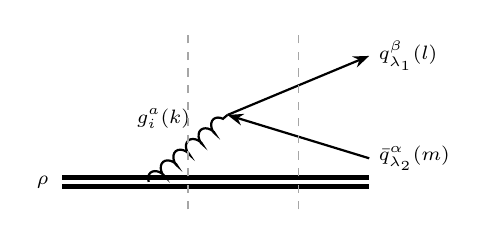
\begin{tikzpicture}
\draw[val] (0,0) -- (3.9,0); \node[left] at (-0.05,0) {\scriptsize$\rho$};
\draw[gl] (1.1,0) -- (2.1,0.85); \node[above left] at (1.75,0.55) {\scriptsize$\gl{a}{i}{k}$};
\draw[qk] (2.1,0.85) -- (3.9,1.6); \node[right] at (3.9,1.6) {\scriptsize$\qk{\beta}{\lambda_{1}}{l}$};
\draw[qk] (3.9,0.3) -- (2.1,0.85); \node[right] at (3.9,0.3) {\scriptsize$\aqk{\alpha}{\lambda_{2}}{m}$};
\draw[cut] (1.6,-0.35) -- (1.6,1.95); \draw[cut] (3.0,-0.35) -- (3.0,1.95);
\end{tikzpicture}
\end{center}
Applying the LCPT rules,
\begin{equation}
\ket{\Psi^{1}_{q\bar q\,\rho}}=\int\! d^{3}k\,d^{3}l\,d^{3}m\;
\ket{\qk{\beta}{\lambda_{1}}{l}\aqk{\alpha}{\lambda_{2}}{m}}\;
\frac{\bra{\qk{\beta}{\lambda_{1}}{l}\aqk{\alpha}{\lambda_{2}}{m}}H_{gq\bar q}\ket{\gl{a}{i}{k}}}
{-E_{q\bar q}(l,m)}\;
\frac{\bra{\gl{a}{i}{k}}H_{g}\vac}{-E_{g}(k)} ,
\label{eq:Pvac1def}
\end{equation}
where here and below the sums over colours, polarizations, helicities and flavours are implicit.
Using the matrix elements \eqref{eq:MEqqg} and \eqref{eq:MEg} and $k=l+m$,
\begin{equation}
\ket{\Psi^{1}_{q\bar q\,\rho}}=\frac{g^{2}}{32\pi^{3}}\int\!d^{3}l\,d^{3}m\;
\ket{\qk{\beta}{\lambda_{1}}{l}\aqk{\alpha}{\lambda_{2}}{m}}\;
\frac{t^{a}_{\beta\alpha}\,\rho^{a}(-k)\,k^{i}\,\Ph^{i}_{\lambda_{1}\lambda_{2}}(k;l,m)}
{(k^{+})^{2}\,\eps_{k}\,\big(\eps_{l}+\eps_{m}\big)} .
\label{eq:Pvac1}
\end{equation}

\paragraph{(b) Instantaneous pair creation off the valence charge.}
\begin{center}
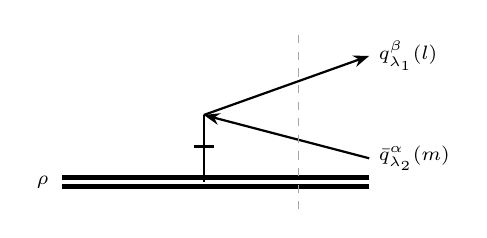
\begin{tikzpicture}
\draw[val] (0,0) -- (3.9,0); \node[left] at (-0.05,0) {\scriptsize$\rho$};
\draw[ins] (1.8,0) -- (1.8,0.85); \ibar{1.8}{0.45}
\draw[qk] (1.8,0.85) -- (3.9,1.6); \node[right] at (3.9,1.6) {\scriptsize$\qk{\beta}{\lambda_{1}}{l}$};
\draw[qk] (3.9,0.3) -- (1.8,0.85); \node[right] at (3.9,0.3) {\scriptsize$\aqk{\alpha}{\lambda_{2}}{m}$};
\draw[cut] (3.0,-0.35) -- (3.0,1.95);
\end{tikzpicture}
\end{center}
This is the $\rho\cdot J_{q}$ term of $H_{q-{\rm inst}}$, Eq.~\eqref{eq:Hqinst}:
\begin{multline}
\ket{\Psi^{2}_{q\bar q\,\rho}}=\int\! d^{3}l\,d^{3}m\;
\ket{\qk{\beta}{\lambda_{1}}{l}\aqk{\alpha}{\lambda_{2}}{m}}\;
\frac{\bra{\qk{\beta}{\lambda_{1}}{l}\aqk{\alpha}{\lambda_{2}}{m}}H_{q-{\rm inst}}\vac}{-E_{q\bar q}(l,m)}
\\
=-\frac{g^{2}}{8\pi^{3}}\int\!d^{3}l\,d^{3}m\;
\ket{q\bar q}\;
\frac{t^{a}_{\beta\alpha}\,\rho^{a}(-k)\,\delta_{\lambda_{1}\lambda_{2}}}
{(k^{+})^{2}\,\big(\eps_{l}+\eps_{m}\big)} ,
\label{eq:Pvac2}
\end{multline}
with $k\equiv l+m$ and the matrix element \eqref{eq:MEinst}.

\subsubsection{Summary of results}
\label{sec:sum-vac}

Using
$k^{i}\Gam^{i}(k;l,m)=4\eps_{k}-2(\eps_{l}+\eps_{m})-\tfrac{k^{+}}{l^{+}m^{+}}(\bm\sigma\!\cdot\!\bm l)(\bm\sigma\!\cdot\!\bm m)$,
which follows from \eqref{eq:Phi} and $\bm k=\bm l+\bm m$, the term proportional to $\eps_{k}$ in
\eqref{eq:Pvac1} cancels the instantaneous contribution \eqref{eq:Pvac2} exactly, and the quark
component of the vacuum at order $g^{2}$ is
\begin{equation}
\ket{\Psi_{q\bar q\,\rho}}=-\frac{g^{2}}{8\pi^{3}}\int\!d^{3}l\,d^{3}m\;
\ket{\qk{\beta}{\lambda_{1}}{l}\aqk{\alpha}{\lambda_{2}}{m}}\;
t^{a}_{\beta\alpha}\rho^{a}(-k)\left[\frac{\delta_{\lambda_{1}\lambda_{2}}}{k^{+}\bm k^{2}}
+\frac{\chi^{\dg}_{\lambda_{1}}(\bm\sigma\!\cdot\!\bm l)(\bm\sigma\!\cdot\!\bm m)\chi_{\lambda_{2}}}
{2\,l^{+}m^{+}\bm k^{2}\,(\eps_{l}+\eps_{m})}\right].
\label{eq:Pvac}
\end{equation}
The cancellation of the instantaneous term is required by unitarity: the relation
\eqref{eq:UA2} contains no instantaneous piece. Since the pair component is of order $g^{2}$, its
norm is of order $g^{4}$, and the normalization $N$ of the vacuum is not modified by quarks at the
order we work. The full vacuum state through $\order{g^{2}}$ is the one of Paper~I supplemented by
\eqref{eq:Pvac}, with $\rho=\rho_{g}+\rho_{q}$ in all the gluonic components.

%----------------------------------------------------------------------
\subsection{Calculation of the single-gluon incoming state}
\label{sec:wf-g}
%----------------------------------------------------------------------

We now examine all quark contributions at orders $g$ and $g^{2}$ associated with a single-gluon
incoming state $\ket{\gl{a}{i}{k}}$. The possible final configurations are a quark--antiquark pair
(order $g$), the one gluon state itself (through the quark loop) and the quark--antiquark--gluon
state (order $g^{2}$).

\subsubsection{Quark--antiquark outgoing}

To order $g$ only one diagram contributes: the incoming gluon splits into a pair.
\begin{center}
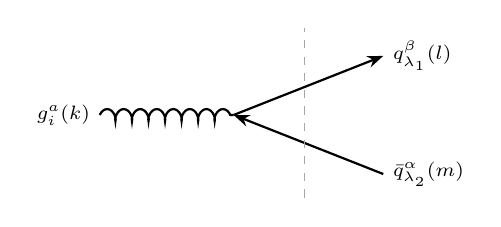
\begin{tikzpicture}
\draw[gl] (0,0.85) -- (1.7,0.85); \node[left] at (0,0.85) {\scriptsize$\gl{a}{i}{k}$};
\draw[qk] (1.7,0.85) -- (3.6,1.6); \node[right] at (3.6,1.6) {\scriptsize$\qk{\beta}{\lambda_{1}}{l}$};
\draw[qk] (3.6,0.1) -- (1.7,0.85); \node[right] at (3.6,0.1) {\scriptsize$\aqk{\alpha}{\lambda_{2}}{m}$};
\draw[cut] (2.6,-0.2) -- (2.6,1.95);
\end{tikzpicture}
\end{center}
\begin{multline}
\ket{(\Psi^{a}_{i}(k))_{q\bar q}}=\int\! d^{3}l\,d^{3}m\;
\ket{\qk{\beta}{\lambda_{1}}{l}\aqk{\alpha}{\lambda_{2}}{m}}\;
\frac{\bra{\qk{\beta}{\lambda_{1}}{l}\aqk{\alpha}{\lambda_{2}}{m}}H_{gq\bar q}\ket{\gl{a}{i}{k}}}
{E_{g}(k)-E_{q\bar q}(l,m)}
\\
=\frac{g}{8\pi^{3/2}}\int\! d^{3}l\,d^{3}m\;\ket{q\bar q}\;
\frac{t^{a}_{\beta\alpha}\,\dthree(k-l-m)\,\Ph^{i}_{\lambda_{1}\lambda_{2}}(k;l,m)}
{\sqrt{k^{+}}\;\big(\eps_{k}-\eps_{l}-\eps_{m}\big)} .
\label{eq:Pg}
\end{multline}

\subsubsection{One gluon outgoing: the quark loop}

At order $g^{2}$ the incoming gluon can fluctuate into a pair and recombine. Since momentum is
conserved along the soft line, this contribution is proportional to $\dthree(k-k')$ and has
$E_{i}=E_{f}$: it is the quark loop contribution to the gluon self-energy, and it enters the
coefficient $B_{3}$ of Paper~I only through its momentum diagonal part. As in Paper~I, its effect
at $\order{g^{2}}$ is fixed by the normalization of the dressed state. The norm of the component
\eqref{eq:Pg} is evaluated with the variables $z=l^{+}/k^{+}$, $\bm\kappa=\bm l-z\bm k$ of
Eq.~\eqref{eq:kappa}, for which $d^{3}l=k^{+}dz\,d^{2}\kappa$ and, for fixed $i$ after averaging over the direction of
$\bm\kappa$,
\begin{equation}
\sum_{\lambda_{1}\lambda_{2}}\big|\Ph^{i}_{\lambda_{1}\lambda_{2}}(k;l,m)\big|^{2}
=\frac{2\,\bm\kappa^{2}\,\big[z^{2}+(1-z)^{2}\big]}{(k^{+})^{2}z^{2}(1-z)^{2}} .
\label{eq:PhiSq}
\end{equation}
All powers of $\bm\kappa$ and $k^{+}$ cancel against the energy denominator and one finds
\begin{align}
\big\langle(\Psi^{a'}_{i'}(k'))_{q\bar q}\big|(\Psi^{a}_{i}(k))_{q\bar q}\big\rangle
&=\delta^{aa'}\delta_{ii'}\dthree(k-k')\,\frac{g^{2}\Nf T_{F}}{8\pi^{3}}
\int_{\Lambda/k^{+}}^{1-\Lambda/k^{+}}\!\!dz\,\big[z^{2}+(1-z)^{2}\big]\int\!\frac{d^{2}\kappa}{\bm\kappa^{2}}
\nonumber\\
&=\delta^{aa'}\delta_{ii'}\dthree(k-k')\,\frac{g^{2}\Nf T_{F}}{8\pi^{3}}\,\frac{2}{3}\int\!\frac{d^{2}\kappa}{\bm\kappa^{2}},
\label{eq:qloop}
\end{align}
with $T_{F}=1/2$; the longitudinal integral is finite and the cutoff $\Lambda$ may be removed.
Combined with the gluon loop of Paper~I, Eq.~(4.83) there, the order $g^{2}$ norm of the
two-parton components of a soft gluon is
\begin{equation}
\frac{g^{2}}{8\pi^{3}}\left[2N_{c}\log\frac{k^{+}}{\Lambda}-\frac{11N_{c}-4T_{F}\Nf}{6}\right]
\int\!\frac{d^{2}\kappa}{\bm\kappa^{2}},
\label{eq:gnorm}
\end{equation}
in which the familiar combination $11N_{c}-4T_{F}\Nf$ of the one-loop $\beta$-function appears as
the coefficient of the ultraviolet divergence. The transverse integral is scaleless and vanishes
in dimensional regularization. Therefore, exactly as in Paper~I, the quark loop does not modify
the normalization $N$ at $\order{g^{2}}$, and the momentum diagonal part of $B_{3}$ is unchanged.

\subsubsection{Quark, antiquark and one gluon outgoing}

At order $g^{2}$ there are seven connected contributions to the
$\ket{\qk{\beta}{\lambda_{1}}{l}\aqk{\alpha}{\lambda_{2}}{m}\gl{d}{n}{r}}$ component. We denote the
overall energy denominator by
\begin{equation}
D_{f}\equiv E_{i}-E_{f}=\eps_{k}-\eps_{l}-\eps_{m}-\eps_{r} .
\end{equation}

\paragraph{(a) The gluon splits into a pair, then the quark emits a gluon.}
\begin{center}
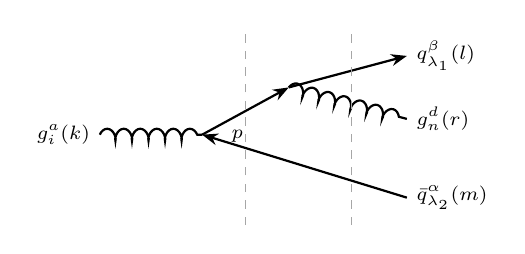
\begin{tikzpicture}
\draw[gl] (0,0.9) -- (1.3,0.9); \node[left] at (0,0.9) {\scriptsize$\gl{a}{i}{k}$};
\draw[qk] (1.3,0.9) -- (2.4,1.5); \node[below right] at (1.55,1.08) {\scriptsize$p$};
\draw[qk] (2.4,1.5) -- (3.9,1.9); \node[right] at (3.9,1.9) {\scriptsize$\qk{\beta}{\lambda_{1}}{l}$};
\draw[gl] (2.4,1.5) -- (3.9,1.1); \node[right] at (3.9,1.1) {\scriptsize$\gl{d}{n}{r}$};
\draw[qk] (3.9,0.1) -- (1.3,0.9); \node[right] at (3.9,0.1) {\scriptsize$\aqk{\alpha}{\lambda_{2}}{m}$};
\draw[cut] (1.85,-0.25) -- (1.85,2.25); \draw[cut] (3.2,-0.25) -- (3.2,2.25);
\end{tikzpicture}
\end{center}
\begin{multline}
\ket{(\Psi^{a}_{i}(k))^{1}_{gq\bar q}}=\int\! d^{3}p\,d^{3}l\,d^{3}m\,d^{3}r\;
\ket{q\bar q\,g}\;
\\
\frac{\bra{\qk{\beta}{\lambda_{1}}{l}\gl{d}{n}{r}}H_{gq\bar q}\ket{\qk{\gamma}{\lambda}{p}}}{D_{f}}\;
\frac{\bra{\qk{\gamma}{\lambda}{p}\aqk{\alpha}{\lambda_{2}}{m}}H_{gq\bar q}\ket{\gl{a}{i}{k}}}
{\eps_{k}-\eps_{p}-\eps_{m}} .
\end{multline}
Using \eqref{eq:MEqqg} and \eqref{eq:MEqg}, closing the intermediate helicity sum with
$\sum_{\lambda}\chi_{\lambda}\chi^{\dg}_{\lambda}=\mathbf 1$, and $p=l+r$,
\begin{multline}
\ket{(\Psi^{a}_{i}(k))^{1}_{gq\bar q}}=\frac{g^{2}}{64\pi^{3}}\int\! d^{3}l\,d^{3}m\,d^{3}r\;
\ket{q\bar q\,g}\\
\times\,(t^{d}t^{a})_{\beta\alpha}\,\frac{\dthree(k-l-m-r)}{\sqrt{r^{+}k^{+}}}\,
\frac{\chi^{\dg}_{\lambda_{1}}\Gam^{n}(r;l,p)\,\Gam^{i}(k;p,m)\chi_{\lambda_{2}}}
{D_{f}\,\big(\eps_{k}-\eps_{p}-\eps_{m}\big)} .
\label{eq:B3a}
\end{multline}

\paragraph{(b) The gluon splits into a pair, then the antiquark emits a gluon.}
\begin{center}
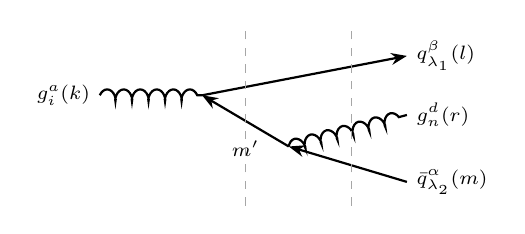
\begin{tikzpicture}
\draw[gl] (0,1.6) -- (1.3,1.6); \node[left] at (0,1.6) {\scriptsize$\gl{a}{i}{k}$};
\draw[qk] (1.3,1.6) -- (3.9,2.1); \node[right] at (3.9,2.1) {\scriptsize$\qk{\beta}{\lambda_{1}}{l}$};
\draw[qk] (2.4,0.95) -- (1.3,1.6); \node[below] at (1.85,1.15) {\scriptsize$m'$};
\draw[qk] (3.9,0.5) -- (2.4,0.95); \node[right] at (3.9,0.5) {\scriptsize$\aqk{\alpha}{\lambda_{2}}{m}$};
\draw[gl] (2.4,0.95) -- (3.9,1.35); \node[right] at (3.9,1.35) {\scriptsize$\gl{d}{n}{r}$};
\draw[cut] (1.85,0.2) -- (1.85,2.45); \draw[cut] (3.2,0.2) -- (3.2,2.45);
\end{tikzpicture}
\end{center}
With $m'=m+r$, the antiquark vertex \eqref{eq:MEaqg} and the same steps,
\begin{multline}
\ket{(\Psi^{a}_{i}(k))^{2}_{gq\bar q}}=-\frac{g^{2}}{64\pi^{3}}\int\! d^{3}l\,d^{3}m\,d^{3}r\;
\ket{q\bar q\,g}\\
\times\,(t^{a}t^{d})_{\beta\alpha}\,\frac{\dthree(k-l-m-r)}{\sqrt{r^{+}k^{+}}}\,
\frac{\chi^{\dg}_{\lambda_{1}}\Gam^{i}(k;l,m')\,\Gam^{n}(r;m',m)\chi_{\lambda_{2}}}
{D_{f}\,\big(\eps_{k}-\eps_{l}-\eps_{m'}\big)} .
\label{eq:B3b}
\end{multline}

\paragraph{(c) The gluon splits into two gluons, one of which splits into a pair.}
\begin{center}
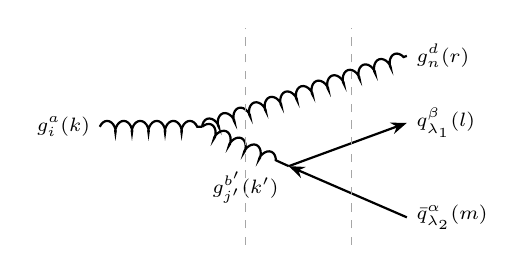
\begin{tikzpicture}
\draw[gl] (0,1.1) -- (1.3,1.1); \node[left] at (0,1.1) {\scriptsize$\gl{a}{i}{k}$};
\draw[gl] (1.3,1.1) -- (3.9,2.0); \node[right] at (3.9,2.0) {\scriptsize$\gl{d}{n}{r}$};
\draw[gl] (1.3,1.1) -- (2.4,0.6); \node[below] at (1.85,0.65) {\scriptsize$\gl{b'}{j'}{k'}$};
\draw[qk] (2.4,0.6) -- (3.9,1.15); \node[right] at (3.9,1.15) {\scriptsize$\qk{\beta}{\lambda_{1}}{l}$};
\draw[qk] (3.9,-0.05) -- (2.4,0.6); \node[right] at (3.9,-0.05) {\scriptsize$\aqk{\alpha}{\lambda_{2}}{m}$};
\draw[cut] (1.85,-0.4) -- (1.85,2.35); \draw[cut] (3.2,-0.4) -- (3.2,2.35);
\end{tikzpicture}
\end{center}
\begin{equation}
\ket{(\Psi^{a}_{i}(k))^{3}_{gq\bar q}}=\frac12\int\! d^{3}k'\,d^{3}l\,d^{3}m\,d^{3}r\;
\ket{q\bar q\,g}\;
\frac{\bra{q\bar q}H_{gq\bar q}\ket{\gl{b'}{j'}{k'}}}{D_{f}}\;
\frac{\bra{\gl{b'}{j'}{k'}\gl{d}{n}{r}}H_{ggg}\ket{\gl{a}{i}{k}}}{\eps_{k}-\eps_{k'}-\eps_{r}} .
\end{equation}
The factor $\tfrac12$ cancels against the two assignments of the intermediate gluon pair. With
$k'=l+m$ and \eqref{eq:MEggg},
\begin{multline}
\ket{(\Psi^{a}_{i}(k))^{3}_{gq\bar q}}=\frac{ig^{2}}{64\pi^{3}}\int\! d^{3}l\,d^{3}m\,d^{3}r\;
\ket{q\bar q\,g}\\
\times\,f^{ab'd}t^{b'}_{\beta\alpha}\,\frac{\dthree(k-l-m-r)}{k'^{+}\sqrt{k^{+}r^{+}}}\,
\frac{\Vg^{ij'n}(k;k',r)\;\Ph^{j'}_{\lambda_{1}\lambda_{2}}(k';l,m)}
{D_{f}\,\big(\eps_{k}-\eps_{k'}-\eps_{r}\big)} .
\label{eq:B3c}
\end{multline}

\paragraph{(d), (e) The valence emits the gluon $r$ and the incoming gluon splits.}
\begin{center}
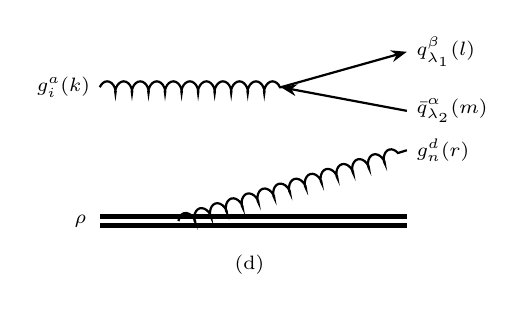
\begin{tikzpicture}
\draw[val] (0,0) -- (3.9,0); \node[left] at (-0.05,0) {\scriptsize$\rho$};
\draw[gl] (0,1.7) -- (2.3,1.7); \node[left] at (0,1.7) {\scriptsize$\gl{a}{i}{k}$};
\draw[gl] (1.0,0) -- (3.9,0.9); \node[right] at (3.9,0.9) {\scriptsize$\gl{d}{n}{r}$};
\draw[qk] (2.3,1.7) -- (3.9,2.15); \node[right] at (3.9,2.15) {\scriptsize$\qk{\beta}{\lambda_{1}}{l}$};
\draw[qk] (3.9,1.4) -- (2.3,1.7); \node[right] at (3.9,1.4) {\scriptsize$\aqk{\alpha}{\lambda_{2}}{m}$};
\node at (1.9,-0.55) {\scriptsize (d)};
\end{tikzpicture}
\hspace{0.7cm}
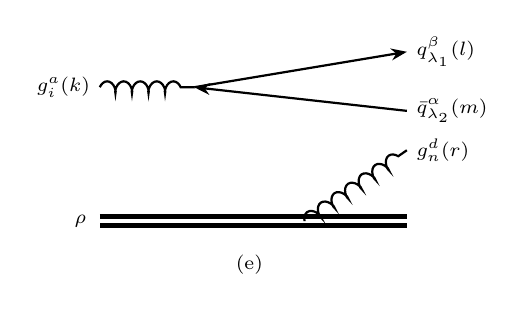
\begin{tikzpicture}
\draw[val] (0,0) -- (3.9,0); \node[left] at (-0.05,0) {\scriptsize$\rho$};
\draw[gl] (0,1.7) -- (1.2,1.7); \node[left] at (0,1.7) {\scriptsize$\gl{a}{i}{k}$};
\draw[gl] (2.6,0) -- (3.9,0.9); \node[right] at (3.9,0.9) {\scriptsize$\gl{d}{n}{r}$};
\draw[qk] (1.2,1.7) -- (3.9,2.15); \node[right] at (3.9,2.15) {\scriptsize$\qk{\beta}{\lambda_{1}}{l}$};
\draw[qk] (3.9,1.4) -- (1.2,1.7); \node[right] at (3.9,1.4) {\scriptsize$\aqk{\alpha}{\lambda_{2}}{m}$};
\node at (1.9,-0.55) {\scriptsize (e)};
\end{tikzpicture}
\end{center}
In (d) the valence emits first and the intermediate state is
$\ket{\gl{a}{i}{k}\gl{d}{n}{r}}$, with $E_{i}-E_{m}=-\eps_{r}$; in (e) the pair is formed first, with
$E_{i}-E_{m}=\eps_{k}-\eps_{l}-\eps_{m}$:
\begin{align}
\ket{(\Psi^{a}_{i}(k))^{4}_{gq\bar q\,\rho}}&=\int\!d^{3}l\,d^{3}m\,d^{3}r\;\ket{q\bar q\,g}\;
\frac{\bra{q\bar q\,\gl{d}{n}{r}}H_{gq\bar q}\ket{\gl{a}{i}{k}\gl{d}{n}{r}}}{D_{f}}\;
\frac{\bra{\gl{a}{i}{k}\gl{d}{n}{r}}H_{g}\ket{\gl{a}{i}{k}}}{-\eps_{r}},
\\
\ket{(\Psi^{a}_{i}(k))^{5}_{gq\bar q\,\rho}}&=\int\!d^{3}l\,d^{3}m\,d^{3}r\;\ket{q\bar q\,g}\;
\frac{\bra{q\bar q\,\gl{d}{n}{r}}H_{g}\ket{q\bar q}}{D_{f}}\;
\frac{\bra{q\bar q}H_{gq\bar q}\ket{\gl{a}{i}{k}}}{\eps_{k}-\eps_{l}-\eps_{m}} .
\end{align}
Since $D_{f}=(\eps_{k}-\eps_{l}-\eps_{m})+(-\eps_{r})$, the two orderings combine by
\eqref{eq:factor} and the overall denominator cancels:
\begin{equation}
\ket{(\Psi^{a}_{i}(k))^{4+5}_{gq\bar q\,\rho}}=\frac{g^{2}}{32\pi^{3}}\int\!d^{3}l\,d^{3}m\,d^{3}r\;
\ket{q\bar q\,g}\;
\frac{t^{a}_{\beta\alpha}\,r^{n}\rho^{d}(-r)\,\Ph^{i}_{\lambda_{1}\lambda_{2}}(k;l,m)\,\dthree(k-l-m)}
{\sqrt{k^{+}}(r^{+})^{3/2}\,(-\eps_{r})\,\big(\eps_{k}-\eps_{l}-\eps_{m}\big)} .
\label{eq:B3de}
\end{equation}

\paragraph{(f) Instantaneous quark exchange.}
\begin{center}
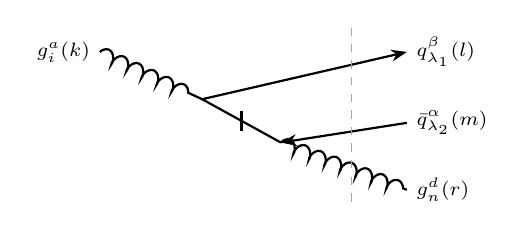
\begin{tikzpicture}
\draw[gl] (0,1.9) -- (1.3,1.3); \node[left] at (0,1.9) {\scriptsize$\gl{a}{i}{k}$};
\draw[gl] (2.3,0.75) -- (3.9,0.15); \node[right] at (3.9,0.15) {\scriptsize$\gl{d}{n}{r}$};
\draw[qk] (1.3,1.3) -- (3.9,1.9); \node[right] at (3.9,1.9) {\scriptsize$\qk{\beta}{\lambda_{1}}{l}$};
\draw[ins] (1.3,1.3) -- (2.3,0.75); \ibarh{1.8}{1.025}
\draw[qk] (3.9,1.0) -- (2.3,0.75); \node[right] at (3.9,1.0) {\scriptsize$\aqk{\alpha}{\lambda_{2}}{m}$};
\draw[cut] (3.2,0.0) -- (3.2,2.2);
\end{tikzpicture}
\end{center}
The two orderings of the gluon attachments give instantaneous fermion lines with plus momenta
$l^{+}+r^{+}$ and $-(m^{+}+r^{+})$; using \eqref{eq:MEggqq1},
\begin{multline}
\ket{(\Psi^{a}_{i}(k))^{6}_{gq\bar q}}=\frac{g^{2}}{16\pi^{3}}\int\!d^{3}l\,d^{3}m\,d^{3}r\;
\ket{q\bar q\,g}\\
\times\,
\frac{\dthree(k-l-m-r)}{\sqrt{k^{+}r^{+}}\,D_{f}}\,
\chi^{\dg}_{\lambda_{1}}\!\left[\frac{(t^{d}t^{a})_{\beta\alpha}\sigma^{n}\sigma^{i}}{l^{+}+r^{+}}
-\frac{(t^{a}t^{d})_{\beta\alpha}\sigma^{i}\sigma^{n}}{m^{+}+r^{+}}\right]\chi_{\lambda_{2}} .
\label{eq:B3f}
\end{multline}

\paragraph{(g) Instantaneous gluon exchange between the gluon and quark currents.}
\begin{center}
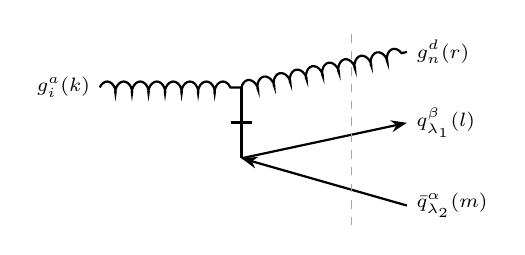
\begin{tikzpicture}
\draw[gl] (0,1.6) -- (1.8,1.6); \node[left] at (0,1.6) {\scriptsize$\gl{a}{i}{k}$};
\draw[gl] (1.8,1.6) -- (3.9,2.05); \node[right] at (3.9,2.05) {\scriptsize$\gl{d}{n}{r}$};
\draw[ins] (1.8,1.6) -- (1.8,0.7); \ibar{1.8}{1.15}
\draw[qk] (1.8,0.7) -- (3.9,1.15); \node[right] at (3.9,1.15) {\scriptsize$\qk{\beta}{\lambda_{1}}{l}$};
\draw[qk] (3.9,0.1) -- (1.8,0.7); \node[right] at (3.9,0.1) {\scriptsize$\aqk{\alpha}{\lambda_{2}}{m}$};
\draw[cut] (3.2,-0.15) -- (3.2,2.35);
\end{tikzpicture}
\end{center}
This is the $J_{g}\cdot J_{q}$ term of \eqref{eq:Hqinst}; the exchanged gluon carries
$P^{+}=l^{+}+m^{+}=k^{+}-r^{+}$ and, with \eqref{eq:MEJJ1},
\begin{equation}
\ket{(\Psi^{a}_{i}(k))^{7}_{gq\bar q}}=\frac{ig^{2}}{2(2\pi)^{3}}\int\!d^{3}l\,d^{3}m\,d^{3}r\;
\ket{q\bar q\,g}\,
\frac{f^{bad}\,t^{b}_{\beta\alpha}\,\delta_{\lambda_{1}\lambda_{2}}\,\delta_{in}\,(k^{+}+r^{+})\,
\dthree(k-l-m-r)}{\sqrt{k^{+}r^{+}}\,(l^{+}+m^{+})^{2}\,D_{f}} .
\label{eq:B3g}
\end{equation}

The remaining topology, in which the valence emits a gluon which splits into the pair while the
incoming gluon is a spectator, is disconnected: it is the $\mf A_{1}$ term of \eqref{eq:Omg} and is
not part of $\mf B_{3}$.

\subsubsection{Summary of results}
\label{sec:sum-g}

The quark components of the dressed one gluon state through $\order{g^{2}}$ are
\begin{equation}
\ket{\Psi^{a}_{i}(k)}\supset\ket{(\Psi^{a}_{i}(k))_{q\bar q}}
+\sum_{n=1,2,3,6,7}\ket{(\Psi^{a}_{i}(k))^{n}_{gq\bar q}}
+\ket{(\Psi^{a}_{i}(k))^{4+5}_{gq\bar q\,\rho}}
+\ket{\gl{a}{i}{k}}\otimes\ket{\Psi_{q\bar q\,\rho}} ,
\label{eq:sum-g}
\end{equation}
where the last term is the vacuum pair component \eqref{eq:Pvac} with the incoming gluon as a
spectator. The diagrams (a)--(c) are the sequential processes $g\to q\bar q\to q\bar q\,g$ and
$g\to gg\to q\bar q\,g$, (d)+(e) is the product of the Weizs\"acker--Williams emission and the
splitting $g\to q\bar q$, and (f), (g) are the two instantaneous interactions. The overall
denominator $D_{f}$ cannot vanish except on the collinear boundary of phase space (a set of
measure zero), so $\mf B_{3}$ has no on-shell pole. As discussed above, the normalization is
unchanged at this order.

%% ---------------- sec4_wf2.tex ----------------
%----------------------------------------------------------------------
\subsection{Calculation of the two-gluon incoming states}
\label{sec:wf-gg}
%----------------------------------------------------------------------

We now examine the quark contributions at order $g^{2}$ associated with an incoming state
containing two gluons, $\ket{\gl{a}{i}{k}\gl{b}{j}{p}}$. The allowed final configurations are a
quark--antiquark pair (virtual corrections to the pair sector and $gg\to q\bar q$ scattering),
a pair with two gluons, and two pairs. The disconnected configurations, in which one of the
incoming gluons is a spectator, reproduce the coefficients $\mf A_{3}$, $\mf A_{1}$ and $\mf B_{3}$
already computed and are not repeated.

\subsubsection{Quark--antiquark outgoing}

The overall energy denominator is
\begin{equation}
D_{f}\equiv\eps_{k}+\eps_{p}-\eps_{l}-\eps_{m}.
\end{equation}
Six topologies contribute.

\paragraph{(a) $s$-channel: the two gluons merge and the resulting gluon splits.}
\begin{center}
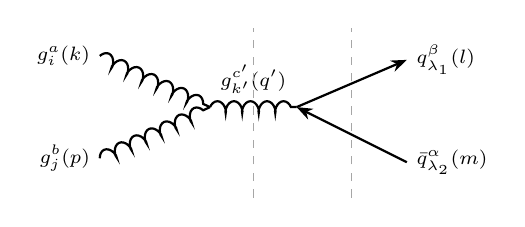
\begin{tikzpicture}
\draw[gl] (0,1.9) -- (1.4,1.25); \node[left] at (0,1.9) {\scriptsize$\gl{a}{i}{k}$};
\draw[gl] (0,0.6) -- (1.4,1.25); \node[left] at (0,0.6) {\scriptsize$\gl{b}{j}{p}$};
\draw[gl] (1.4,1.25) -- (2.5,1.25); \node[above] at (1.95,1.3) {\scriptsize$\gl{c'}{k'}{q'}$};
\draw[qk] (2.5,1.25) -- (3.9,1.85); \node[right] at (3.9,1.85) {\scriptsize$\qk{\beta}{\lambda_{1}}{l}$};
\draw[qk] (3.9,0.55) -- (2.5,1.25); \node[right] at (3.9,0.55) {\scriptsize$\aqk{\alpha}{\lambda_{2}}{m}$};
\draw[cut] (1.95,0.1) -- (1.95,2.25); \draw[cut] (3.2,0.1) -- (3.2,2.25);
\end{tikzpicture}
\end{center}
\begin{equation}
\ket{(\Psi^{ab}_{ij}(k,p))^{1}_{q\bar q}}=\int\! d^{3}q'\,d^{3}l\,d^{3}m\;
\ket{q\bar q}\;
\frac{\bra{q\bar q}H_{gq\bar q}\ket{\gl{c'}{k'}{q'}}}{D_{f}}\;
\frac{\bra{\gl{c'}{k'}{q'}}H_{ggg}\ket{\gl{a}{i}{k}\gl{b}{j}{p}}}{\eps_{k}+\eps_{p}-\eps_{q'}} .
\end{equation}
The $2\to1$ gluon vertex is the Hermitian conjugate of \eqref{eq:MEggg}; with $q'=k+p$,
\begin{multline}
\ket{(\Psi^{ab}_{ij}(k,p))^{1}_{q\bar q}}=-\frac{ig^{2}}{64\pi^{3}}\int\!d^{3}l\,d^{3}m\;
\\
\times\ket{q\bar q}\,f^{abc'}t^{c'}_{\beta\alpha}\,
\frac{\dthree(k+p-l-m)}{q'^{+}\sqrt{k^{+}p^{+}}}\,
\frac{\Vg^{k'ij}(q';k,p)\;\Ph^{k'}_{\lambda_{1}\lambda_{2}}(q';l,m)}
{\big(\eps_{k}+\eps_{p}-\eps_{q'}\big)\,D_{f}} .
\label{eq:B1a}
\end{multline}
This contribution is symmetric under $(a,i,k)\leftrightarrow(b,j,p)$.

\paragraph{(b) One gluon is absorbed by the valence charge, the other splits.}
\begin{center}
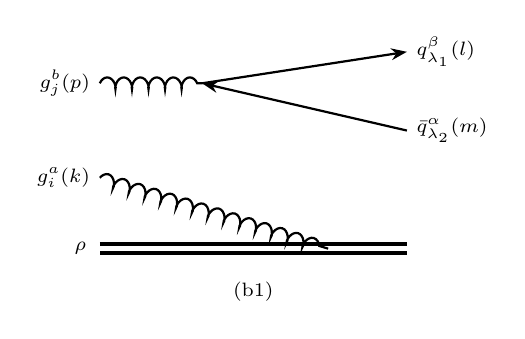
\begin{tikzpicture}
\draw[val] (0,0) -- (3.9,0); \node[left] at (-0.05,0) {\scriptsize$\rho$};
\draw[gl] (0,0.9) -- (2.9,0); \node[left] at (0,0.9) {\scriptsize$\gl{a}{i}{k}$};
\draw[gl] (0,2.1) -- (1.3,2.1); \node[left] at (0,2.1) {\scriptsize$\gl{b}{j}{p}$};
\draw[qk] (1.3,2.1) -- (3.9,2.5); \node[right] at (3.9,2.5) {\scriptsize$\qk{\beta}{\lambda_{1}}{l}$};
\draw[qk] (3.9,1.5) -- (1.3,2.1); \node[right] at (3.9,1.5) {\scriptsize$\aqk{\alpha}{\lambda_{2}}{m}$};
\node at (1.95,-0.55) {\scriptsize (b1)};
\end{tikzpicture}
\hspace{0.5cm}
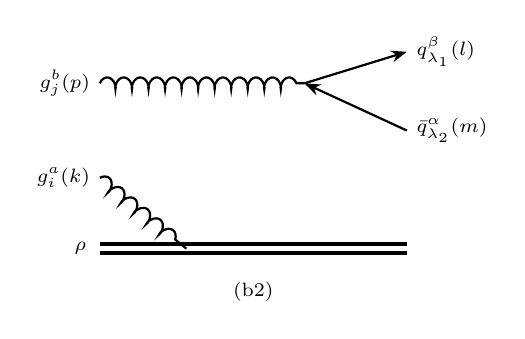
\begin{tikzpicture}
\draw[val] (0,0) -- (3.9,0); \node[left] at (-0.05,0) {\scriptsize$\rho$};
\draw[gl] (0,0.9) -- (1.1,0); \node[left] at (0,0.9) {\scriptsize$\gl{a}{i}{k}$};
\draw[gl] (0,2.1) -- (2.6,2.1); \node[left] at (0,2.1) {\scriptsize$\gl{b}{j}{p}$};
\draw[qk] (2.6,2.1) -- (3.9,2.5); \node[right] at (3.9,2.5) {\scriptsize$\qk{\beta}{\lambda_{1}}{l}$};
\draw[qk] (3.9,1.5) -- (2.6,2.1); \node[right] at (3.9,1.5) {\scriptsize$\aqk{\alpha}{\lambda_{2}}{m}$};
\node at (1.95,-0.55) {\scriptsize (b2)};
\end{tikzpicture}
\end{center}
In (b1) the intermediate state is $\ket{q\bar q\,\gl{a}{i}{k}}$, with
$E_{i}-E_{m}=\eps_{p}-\eps_{l}-\eps_{m}$; in (b2) it is $\ket{\gl{b}{j}{p}}$, with $E_{i}-E_{m}=\eps_{k}$:
\begin{align}
\ket{(\Psi^{ab}_{ij}(k,p))^{2}_{q\bar q\,\rho}}&=\int\!d^{3}l\,d^{3}m\;\ket{q\bar q}\;
\frac{\bra{q\bar q}H_{g}\ket{q\bar q\,\gl{a}{i}{k}}}{D_{f}}\;
\frac{\bra{q\bar q\,\gl{a}{i}{k}}H_{gq\bar q}\ket{\gl{a}{i}{k}\gl{b}{j}{p}}}{\eps_{p}-\eps_{l}-\eps_{m}},
\\
\ket{(\Psi^{ab}_{ij}(k,p))^{3}_{q\bar q\,\rho}}&=\int\!d^{3}l\,d^{3}m\;\ket{q\bar q}\;
\frac{\bra{q\bar q}H_{gq\bar q}\ket{\gl{b}{j}{p}}}{D_{f}}\;
\frac{\bra{\gl{b}{j}{p}}H_{g}\ket{\gl{a}{i}{k}\gl{b}{j}{p}}}{\eps_{k}} .
\end{align}
Since $D_{f}=(\eps_{p}-\eps_{l}-\eps_{m})+\eps_{k}$, the two orderings combine by \eqref{eq:factor},
\begin{multline}
\ket{(\Psi^{ab}_{ij}(k,p))^{2+3}_{q\bar q\,\rho}}=\frac{g^{2}}{32\pi^{3}}\int\!d^{3}l\,d^{3}m\;
\ket{q\bar q}\;
\frac{\rho^{a}(k)\,t^{b}_{\beta\alpha}\,k^{i}\,\Ph^{j}_{\lambda_{1}\lambda_{2}}(p;l,m)\,\dthree(p-l-m)}
{(k^{+})^{3/2}\sqrt{p^{+}}\;\eps_{k}\,\big(\eps_{p}-\eps_{l}-\eps_{m}\big)}\\
+\big((a,i,k)\leftrightarrow(b,j,p)\big) .
\label{eq:B1b}
\end{multline}

\paragraph{(c) $t$-channel quark exchange: one gluon splits and the quark absorbs the other.}
\begin{center}
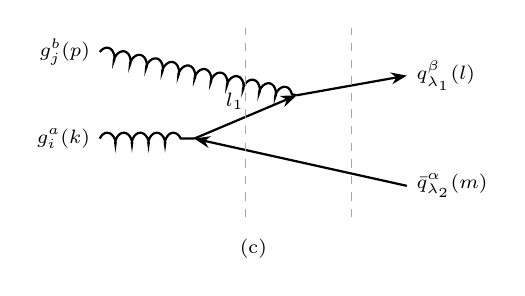
\begin{tikzpicture}
\draw[gl] (0,1.5) -- (1.2,1.5); \node[left] at (0,1.5) {\scriptsize$\gl{a}{i}{k}$};
\draw[qk] (1.2,1.5) -- (2.5,2.05); \node[above left] at (1.95,1.75) {\scriptsize$l_{1}$};
\draw[qk] (2.5,2.05) -- (3.9,2.3); \node[right] at (3.9,2.3) {\scriptsize$\qk{\beta}{\lambda_{1}}{l}$};
\draw[qk] (3.9,0.9) -- (1.2,1.5); \node[right] at (3.9,0.9) {\scriptsize$\aqk{\alpha}{\lambda_{2}}{m}$};
\draw[gl] (0,2.6) -- (2.5,2.05); \node[left] at (0,2.6) {\scriptsize$\gl{b}{j}{p}$};
\draw[cut] (1.85,0.5) -- (1.85,2.9); \draw[cut] (3.2,0.5) -- (3.2,2.9);
\node at (1.95,0.1) {\scriptsize (c)};
\end{tikzpicture}
\hspace{0.8cm}
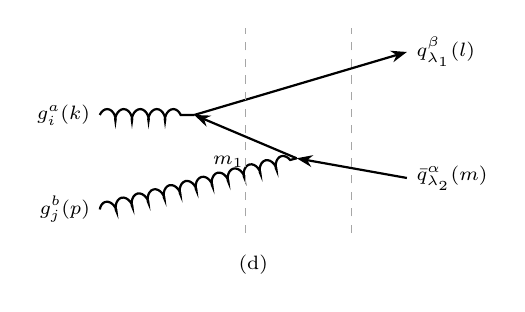
\begin{tikzpicture}
\draw[gl] (0,1.5) -- (1.2,1.5); \node[left] at (0,1.5) {\scriptsize$\gl{a}{i}{k}$};
\draw[qk] (1.2,1.5) -- (3.9,2.3); \node[right] at (3.9,2.3) {\scriptsize$\qk{\beta}{\lambda_{1}}{l}$};
\draw[qk] (2.5,0.95) -- (1.2,1.5); \node[below left] at (1.95,1.1) {\scriptsize$m_{1}$};
\draw[qk] (3.9,0.7) -- (2.5,0.95); \node[right] at (3.9,0.7) {\scriptsize$\aqk{\alpha}{\lambda_{2}}{m}$};
\draw[gl] (0,0.3) -- (2.5,0.95); \node[left] at (0,0.3) {\scriptsize$\gl{b}{j}{p}$};
\draw[cut] (1.85,0.0) -- (1.85,2.6); \draw[cut] (3.2,0.0) -- (3.2,2.6);
\node at (1.95,-0.4) {\scriptsize (d)};
\end{tikzpicture}
\end{center}
The gluon $k$ splits into $\qk{\gamma}{\lambda}{l_{1}}\aqk{\alpha}{\lambda_{2}}{m}$ and the quark absorbs
the gluon $p$, so that $l_{1}=l-p$ and the process requires $l^{+}>p^{+}$. The absorption vertex
is the Hermitian conjugate of \eqref{eq:MEqg}, $\big[\Ph^{j}_{\lambda'\lambda}(p;l_{1},l)\big]^{*}
=\Ph^{j}_{\lambda\lambda'}(p;l,l_{1})$:
\begin{align}
\ket{(\Psi^{ab}_{ij}(k,p))^{4}_{q\bar q}}&=\int\!d^{3}l_{1}\,d^{3}l\,d^{3}m\;\ket{q\bar q}\;
\frac{\bra{\qk{\beta}{\lambda_{1}}{l}}H_{gq\bar q}\ket{\qk{\gamma}{\lambda}{l_{1}}\gl{b}{j}{p}}}{D_{f}}
\nonumber\\&\hspace{3.2cm}\times
\frac{\bra{\qk{\gamma}{\lambda}{l_{1}}\aqk{\alpha}{\lambda_{2}}{m}}H_{gq\bar q}\ket{\gl{a}{i}{k}}}
{\eps_{k}-\eps_{l_{1}}-\eps_{m}}
\nonumber\\
&=\frac{g^{2}}{64\pi^{3}}\int\!d^{3}l\,d^{3}m\;\ket{q\bar q}\;(t^{b}t^{a})_{\beta\alpha}\,
\frac{\dthree(k+p-l-m)\,\theta(l^{+}-p^{+})}{\sqrt{k^{+}p^{+}}}
\nonumber\\&\hspace{3.2cm}\times
\frac{\chi^{\dg}_{\lambda_{1}}\Gam^{j}(p;l,l_{1})\,\Gam^{i}(k;l_{1},m)\chi_{\lambda_{2}}}
{\big(\eps_{k}-\eps_{l_{1}}-\eps_{m}\big)\,D_{f}}
\nonumber\\
&\quad+\big((a,i,k)\leftrightarrow(b,j,p)\big).
\label{eq:B1c}
\end{align}

\paragraph{(d) $u$-channel quark exchange: one gluon splits and the antiquark absorbs the other.}
Now $m_{1}=m-p$, the process requires $m^{+}>p^{+}$, and the antiquark vertex \eqref{eq:MEaqg}
supplies a minus sign:
\begin{multline}
\ket{(\Psi^{ab}_{ij}(k,p))^{5}_{q\bar q}}=-\frac{g^{2}}{64\pi^{3}}\int\!d^{3}l\,d^{3}m\;\ket{q\bar q}\;\\
\times(t^{a}t^{b})_{\beta\alpha}\,
\frac{\dthree(k+p-l-m)\,\theta(m^{+}-p^{+})}{\sqrt{k^{+}p^{+}}}\,
\frac{\chi^{\dg}_{\lambda_{1}}\Gam^{i}(k;l,m_{1})\,\Gam^{j}(p;m_{1},m)\chi_{\lambda_{2}}}
{\big(\eps_{k}-\eps_{l}-\eps_{m_{1}}\big)\,D_{f}}\\
+\big((a,i,k)\leftrightarrow(b,j,p)\big).
\label{eq:B1d}
\end{multline}
The diagrams (c) and (d) are the light-cone time ordered $t$- and $u$-channel quark exchange
graphs of $gg\to q\bar q$. In the language of the evolution operator they are the products
$\mf F_{2}\,\mf A_{3}$ and $\mf G_{2}\,\mf A_{3}$ in \eqref{eq:reduction}, and they are the origin of
the $\mf F$ and $\mf G$ terms of the unitarity relation \eqref{eq:UB2}.

\paragraph{(e) Instantaneous quark exchange.}
\begin{center}
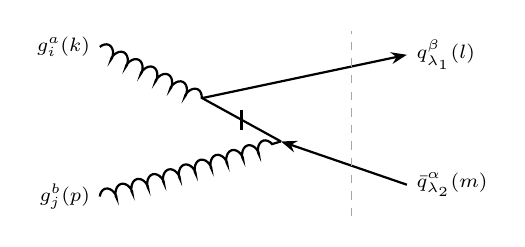
\begin{tikzpicture}
\draw[gl] (0,2.0) -- (1.3,1.35); \node[left] at (0,2.0) {\scriptsize$\gl{a}{i}{k}$};
\draw[gl] (0,0.1) -- (2.3,0.8); \node[left] at (0,0.1) {\scriptsize$\gl{b}{j}{p}$};
\draw[qk] (1.3,1.35) -- (3.9,1.9); \node[right] at (3.9,1.9) {\scriptsize$\qk{\beta}{\lambda_{1}}{l}$};
\draw[ins] (1.3,1.35) -- (2.3,0.8); \ibarh{1.8}{1.075}
\draw[qk] (3.9,0.25) -- (2.3,0.8); \node[right] at (3.9,0.25) {\scriptsize$\aqk{\alpha}{\lambda_{2}}{m}$};
\draw[cut] (3.2,-0.15) -- (3.2,2.2);
\end{tikzpicture}
\end{center}
With \eqref{eq:MEggqq2},
\begin{multline}
\ket{(\Psi^{ab}_{ij}(k,p))^{6}_{q\bar q}}=\frac{g^{2}}{16\pi^{3}}\int\!d^{3}l\,d^{3}m\;\ket{q\bar q}\,
\\
\times\frac{\dthree(k+p-l-m)}{\sqrt{k^{+}p^{+}}\,D_{f}}\,
\chi^{\dg}_{\lambda_{1}}\!\left[\frac{(t^{a}t^{b})_{\beta\alpha}\sigma^{i}\sigma^{j}}{l^{+}-k^{+}}
+\frac{(t^{b}t^{a})_{\beta\alpha}\sigma^{j}\sigma^{i}}{l^{+}-p^{+}}\right]\chi_{\lambda_{2}} .
\label{eq:B1e}
\end{multline}
The second term is the instantaneous part of the $t$-channel exchange (c) (the fermion line
carries $l_{1}^{+}=l^{+}-p^{+}$) and the first that of the $u$-channel exchange (d) (it carries
$l^{+}-k^{+}=-m_{1}^{+}$); unlike (c) and (d), the instantaneous term has support for either sign
of these momenta.

\paragraph{(f) Instantaneous gluon exchange between the gluon and quark currents.}
\begin{center}
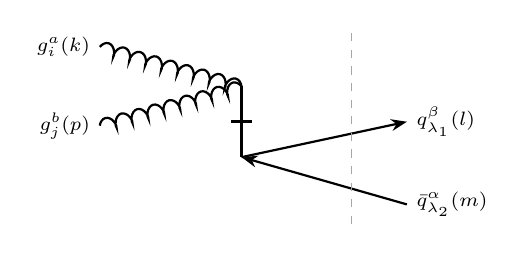
\begin{tikzpicture}
\draw[gl] (0,2.0) -- (1.8,1.5); \node[left] at (0,2.0) {\scriptsize$\gl{a}{i}{k}$};
\draw[gl] (0,1.0) -- (1.8,1.5); \node[left] at (0,1.0) {\scriptsize$\gl{b}{j}{p}$};
\draw[ins] (1.8,1.5) -- (1.8,0.6); \ibar{1.8}{1.05}
\draw[qk] (1.8,0.6) -- (3.9,1.05); \node[right] at (3.9,1.05) {\scriptsize$\qk{\beta}{\lambda_{1}}{l}$};
\draw[qk] (3.9,0.0) -- (1.8,0.6); \node[right] at (3.9,0.0) {\scriptsize$\aqk{\alpha}{\lambda_{2}}{m}$};
\draw[cut] (3.2,-0.25) -- (3.2,2.2);
\end{tikzpicture}
\end{center}
The two incoming gluons are annihilated by $J_{g}$ and the pair is created by $J_{q}$; the
exchanged gluon carries $P^{+}=k^{+}+p^{+}$ and, with \eqref{eq:MEJJ2},
\begin{equation}
\ket{(\Psi^{ab}_{ij}(k,p))^{7}_{q\bar q}}=-\frac{ig^{2}}{2(2\pi)^{3}}\int\!d^{3}l\,d^{3}m\;\ket{q\bar q}\,
\frac{f^{cab}\,t^{c}_{\beta\alpha}\,\delta_{\lambda_{1}\lambda_{2}}\,\delta_{ij}\,(p^{+}-k^{+})\,
\dthree(k+p-l-m)}{\sqrt{k^{+}p^{+}}\,(k^{+}+p^{+})^{2}\,D_{f}} .
\label{eq:B1f}
\end{equation}

\subsubsection{Two gluons, quark and antiquark outgoing}

One incoming gluon splits into the pair and the other into the two outgoing gluons
$\gl{d}{o}{r}\gl{e}{n}{s}$; both time orderings contribute.
\begin{center}
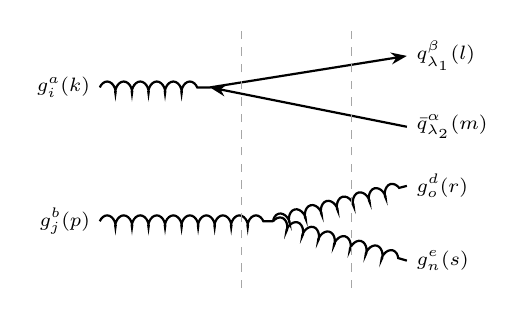
\begin{tikzpicture}
\draw[gl] (0,2.2) -- (1.4,2.2); \node[left] at (0,2.2) {\scriptsize$\gl{a}{i}{k}$};
\draw[qk] (1.4,2.2) -- (3.9,2.6); \node[right] at (3.9,2.6) {\scriptsize$\qk{\beta}{\lambda_{1}}{l}$};
\draw[qk] (3.9,1.7) -- (1.4,2.2); \node[right] at (3.9,1.7) {\scriptsize$\aqk{\alpha}{\lambda_{2}}{m}$};
\draw[gl] (0,0.5) -- (2.2,0.5); \node[left] at (0,0.5) {\scriptsize$\gl{b}{j}{p}$};
\draw[gl] (2.2,0.5) -- (3.9,0.95); \node[right] at (3.9,0.95) {\scriptsize$\gl{d}{o}{r}$};
\draw[gl] (2.2,0.5) -- (3.9,0.0); \node[right] at (3.9,0.0) {\scriptsize$\gl{e}{n}{s}$};
\draw[cut] (1.8,-0.35) -- (1.8,2.95); \draw[cut] (3.2,-0.35) -- (3.2,2.95);
\end{tikzpicture}
\end{center}
With $D_{1}=\eps_{k}-\eps_{l}-\eps_{m}$, $D_{2}=\eps_{p}-\eps_{r}-\eps_{s}$ and $D_{f}=D_{1}+D_{2}$,
\eqref{eq:factor} gives
\begin{align}
\ket{(\Psi^{ab}_{ij}(k,p))_{ggq\bar q}}=\;&\frac{ig^{2}}{64\pi^{3}}\int\!d^{3}l\,d^{3}m\,d^{3}r\,d^{3}s\;
\ket{q\bar q\,\gl{d}{o}{r}\gl{e}{n}{s}}
\nonumber\\&\times t^{a}_{\beta\alpha}f^{bde}\,
\frac{\dthree(k-l-m)\dthree(p-r-s)}{\sqrt{k^{+}p^{+}r^{+}s^{+}}}\,
\frac{\Ph^{i}_{\lambda_{1}\lambda_{2}}(k;l,m)\;\Vg^{jon}(p;r,s)}{D_{1}\,D_{2}}
\nonumber\\&+\big((a,i,k)\leftrightarrow(b,j,p)\big),
\label{eq:Pggqq}
\end{align}
where the factor $\tfrac12$ of the two identical outgoing gluons has cancelled against their two
assignments, as in Paper~I.

\subsubsection{Two quark--antiquark pairs outgoing}

Each gluon splits independently and both orderings again combine by \eqref{eq:factor}:
\begin{align}
\ket{(\Psi^{bc}_{jk}(p,q))_{q\bar qq\bar q}}=\frac{g^{2}}{64\pi^{3}}
\int\!d^{3}l\,d^{3}m\,d^{3}l'\,d^{3}m'\;
&\ket{q\bar q\,q\bar q}\;t^{b}_{\beta\alpha}t^{c}_{\beta'\alpha'}\,
\frac{\dthree(p-l-m)\dthree(q-l'-m')}{\sqrt{p^{+}q^{+}}}
\nonumber\\&\times
\frac{\Ph^{j}_{\lambda_{1}\lambda_{2}}(p;l,m)\;\Ph^{k}_{\lambda_{1}'\lambda_{2}'}(q;l',m')}
{\big(\eps_{p}-\eps_{l}-\eps_{m}\big)\big(\eps_{q}-\eps_{l'}-\eps_{m'}\big)} .
\label{eq:Pqqqq}
\end{align}

\subsubsection{Summary of results}
\label{sec:sum-gg}

The connected quark components of the two-gluon state at order $g^{2}$ are
\begin{multline}
\ket{\Psi^{ab}_{ij}(k,p)}\supset\sum_{n=1,4,5,6,7}\ket{(\Psi^{ab}_{ij}(k,p))^{n}_{q\bar q}}
+\ket{(\Psi^{ab}_{ij}(k,p))^{2+3}_{q\bar q\,\rho}}\\
+\ket{(\Psi^{ab}_{ij}(k,p))_{ggq\bar q}}+\ket{(\Psi^{ab}_{ij}(k,p))_{q\bar qq\bar q}} .
\label{eq:sum-gg}
\end{multline}
The $\rho$ dependent component and the components with four outgoing partons factorize into
products of first order amplitudes. The $\rho$ independent part of the $q\bar q$ component is the
$gg\to q\bar q$ scattering amplitude; its overall denominator $D_{f}$ vanishes on the energy
shell and is understood with the prescription of section~\ref{sec:lcpt}. The new connected
components do not affect the normalization at this order.

%----------------------------------------------------------------------
\subsection{Calculation of the three-gluon incoming states}
\label{sec:wf-ggg}
%----------------------------------------------------------------------

As in Paper~I, we restrict the calculation to the components needed for $\OM$ at
$\order{g^{2}}$. For an incoming state $\ket{\gl{a}{i}{k}\gl{b}{j}{p}\gl{c}{k}{q}}$ the only new
connected quark component is $\ket{q\bar q\,\gl{e}{n}{s}}$: one gluon splits into the pair while
the other two merge.
\begin{center}
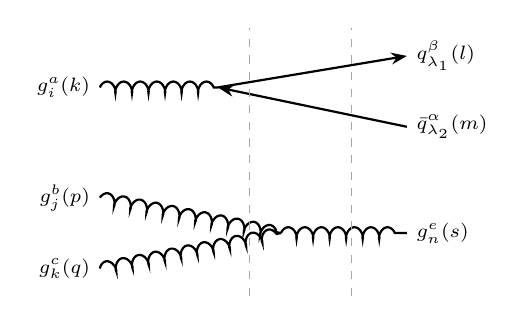
\begin{tikzpicture}
\draw[gl] (0,2.3) -- (1.5,2.3); \node[left] at (0,2.3) {\scriptsize$\gl{a}{i}{k}$};
\draw[qk] (1.5,2.3) -- (3.9,2.7); \node[right] at (3.9,2.7) {\scriptsize$\qk{\beta}{\lambda_{1}}{l}$};
\draw[qk] (3.9,1.8) -- (1.5,2.3); \node[right] at (3.9,1.8) {\scriptsize$\aqk{\alpha}{\lambda_{2}}{m}$};
\draw[gl] (0,0.9) -- (2.3,0.45); \node[left] at (0,0.9) {\scriptsize$\gl{b}{j}{p}$};
\draw[gl] (0,0.0) -- (2.3,0.45); \node[left] at (0,0.0) {\scriptsize$\gl{c}{k}{q}$};
\draw[gl] (2.3,0.45) -- (3.9,0.45); \node[right] at (3.9,0.45) {\scriptsize$\gl{e}{n}{s}$};
\draw[cut] (1.9,-0.35) -- (1.9,3.05); \draw[cut] (3.2,-0.35) -- (3.2,3.05);
\end{tikzpicture}
\end{center}
With $D_{A}=\eps_{k}-\eps_{l}-\eps_{m}$ and $D_{B}=\eps_{p}+\eps_{q}-\eps_{s}$, $D_{A}+D_{B}=D_{f}$,
and \eqref{eq:factor} gives
\begin{align}
\ket{(\Psi^{abc}_{ijk}(k,p,q))_{gq\bar q}}=-\frac{ig^{2}}{64\pi^{3}}
\int\!d^{3}l\,d^{3}m\,d^{3}s\;
&\ket{q\bar q\,\gl{e}{n}{s}}\;t^{a}_{\beta\alpha}f^{ebc}\,
\frac{\dthree(k-l-m)\dthree(s-p-q)}{\sqrt{k^{+}s^{+}p^{+}q^{+}}}
\nonumber\\&\times
\frac{\Ph^{i}_{\lambda_{1}\lambda_{2}}(k;l,m)\;\Vg^{njk}(s;p,q)}{D_{A}\,D_{B}} ,
\label{eq:Pgqq}
\end{align}
summed over the three inequivalent choices of the gluon that splits. Since
$f^{ebc}\Vg^{njk}(s;p,q)$ is symmetric under $(b,j,p)\leftrightarrow(c,k,q)$, a sum over all six
permutations would double count.

\subsubsection{Summary of results}

The only new connected quark component of the three-gluon state at order $g^{2}$ is
\eqref{eq:Pgqq}; it factorizes into the product of the pair splitting amplitude and the
three-gluon merging amplitude of Paper~I.

%% ---------------- sec4_wf3.tex ----------------
%----------------------------------------------------------------------
\subsection{Calculation of the single-quark incoming state}
\label{sec:wf-q}
%----------------------------------------------------------------------

The pure Yang--Mills construction has no analogue of this sector. A soft quark
$\ket{\qk{\beta'}{\lambda'}{l'}}$ emits and absorbs soft gluons and rescatters on the valence
charge; these processes fix the coefficients $\mf F$, $\mf P$, $\mf Q_{1}$ and $\mf K_{1}$. The
results for an incoming antiquark are given at the end of this subsection. The outgoing quark is
$\qk{\beta}{\lambda}{l}$.

\subsubsection{Quark and one gluon outgoing}

To order $g$ the quark emits a soft gluon.
\begin{center}
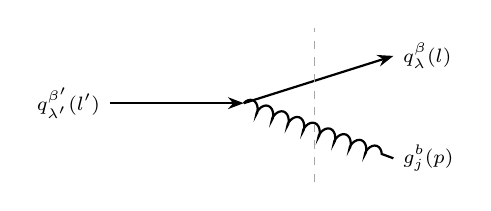
\begin{tikzpicture}
\draw[qk] (0,1.0) -- (1.7,1.0); \node[left] at (0,1.0) {\scriptsize$\qk{\beta'}{\lambda'}{l'}$};
\draw[qk] (1.7,1.0) -- (3.6,1.6); \node[right] at (3.6,1.6) {\scriptsize$\qk{\beta}{\lambda}{l}$};
\draw[gl] (1.7,1.0) -- (3.6,0.3); \node[right] at (3.6,0.3) {\scriptsize$\gl{b}{j}{p}$};
\draw[cut] (2.6,0.0) -- (2.6,1.95);
\end{tikzpicture}
\end{center}
\begin{multline}
\ket{(\Psi^{\beta'}_{\lambda'}(l'))_{qg}}=\int\!d^{3}l\,d^{3}p\;\ket{\qk{\beta}{\lambda}{l}\gl{b}{j}{p}}\,
\frac{\bra{\qk{\beta}{\lambda}{l}\gl{b}{j}{p}}H_{gq\bar q}\ket{\qk{\beta'}{\lambda'}{l'}}}{\eps_{l'}-\eps_{l}-\eps_{p}}\\
=\frac{g}{8\pi^{3/2}}\int\!d^{3}l\,d^{3}p\;\ket{qg}\,
\frac{t^{b}_{\beta\beta'}\,\dthree(l'-l-p)\,\Ph^{j}_{\lambda\lambda'}(p;l,l')}{\sqrt{p^{+}}\,\big(\eps_{l'}-\eps_{l}-\eps_{p}\big)} ,
\label{eq:Pq-qg}
\end{multline}
with the matrix element \eqref{eq:MEqg}. The Weizs\"acker--Williams gluon emitted by $\rho$ with
the quark as a spectator is the disconnected $A$ term of \eqref{eq:Omq}.

\subsubsection{One quark outgoing}

At order $g^{2}$ the soft quark exchanges a gluon with the valence charge. Three diagrams
contribute to the transition $l'\to l$ with momentum transfer to the valence; we write
\begin{equation}
\Delta\equiv E_{i}-E_{f}=\eps_{l'}-\eps_{l}.
\end{equation}

\paragraph{(a) The quark emits a gluon which is absorbed by the valence.}
\begin{center}
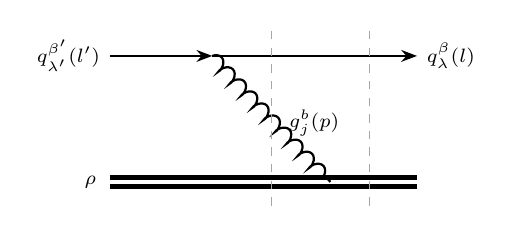
\begin{tikzpicture}
\draw[val] (0,0) -- (3.9,0); \node[left] at (-0.05,0) {\scriptsize$\rho$};
\draw[qk] (0,1.6) -- (1.3,1.6); \node[left] at (0,1.6) {\scriptsize$\qk{\beta'}{\lambda'}{l'}$};
\draw[qk] (1.3,1.6) -- (3.9,1.6); \node[right] at (3.9,1.6) {\scriptsize$\qk{\beta}{\lambda}{l}$};
\draw[gl] (1.3,1.6) -- (2.8,0); \node[right] at (2.15,0.75) {\scriptsize$\gl{b}{j}{p}$};
\draw[cut] (2.05,-0.3) -- (2.05,1.95); \draw[cut] (3.3,-0.3) -- (3.3,1.95);
\end{tikzpicture}
\end{center}
Here $p=l'-l$ and the process requires $l'^{+}>l^{+}$:
\begin{equation}
\ket{(\Psi^{\beta'}_{\lambda'}(l'))^{1}_{q\,\rho}}=\int\!d^{3}l\,d^{3}p\;\ket{\qk{\beta}{\lambda}{l}}\;
\frac{\bra{\qk{\beta}{\lambda}{l}}H_{g}\ket{\qk{\beta}{\lambda}{l}\gl{b}{j}{p}}}{\Delta}\;
\frac{\bra{\qk{\beta}{\lambda}{l}\gl{b}{j}{p}}H_{gq\bar q}\ket{\qk{\beta'}{\lambda'}{l'}}}{\Delta-\eps_{p}} .
\end{equation}
Using \eqref{eq:MEg2} and \eqref{eq:MEqg},
\begin{equation}
\ket{(\Psi^{\beta'}_{\lambda'}(l'))^{1}_{q\,\rho}}=\frac{g^{2}}{32\pi^{3}}\int\!d^{3}l\;\ket{\qk{\beta}{\lambda}{l}}\;
\frac{t^{b}_{\beta\beta'}\,\rho^{b}(p)\,p^{j}\Ph^{j}_{\lambda\lambda'}(p;l,l')}{(p^{+})^{2}\,(\Delta-\eps_{p})\,\Delta}\,
\theta(l'^{+}-l^{+}) .
\label{eq:P1a}
\end{equation}

\paragraph{(b) The valence emits a gluon which is absorbed by the quark.}
\begin{center}
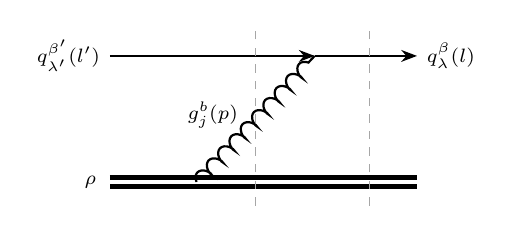
\begin{tikzpicture}
\draw[val] (0,0) -- (3.9,0); \node[left] at (-0.05,0) {\scriptsize$\rho$};
\draw[qk] (0,1.6) -- (2.6,1.6); \node[left] at (0,1.6) {\scriptsize$\qk{\beta'}{\lambda'}{l'}$};
\draw[qk] (2.6,1.6) -- (3.9,1.6); \node[right] at (3.9,1.6) {\scriptsize$\qk{\beta}{\lambda}{l}$};
\draw[gl] (1.1,0) -- (2.6,1.6); \node[left] at (1.75,0.85) {\scriptsize$\gl{b}{j}{p}$};
\draw[cut] (1.85,-0.3) -- (1.85,1.95); \draw[cut] (3.3,-0.3) -- (3.3,1.95);
\end{tikzpicture}
\end{center}
Now $p=l-l'$, the process requires $l^{+}>l'^{+}$ and the intermediate state
$\ket{\qk{\beta'}{\lambda'}{l'}\gl{b}{j}{p}}$ has $E_{i}-E_{m}=-\eps_{p}$:
\begin{equation}
\ket{(\Psi^{\beta'}_{\lambda'}(l'))^{2}_{q\,\rho}}=-\frac{g^{2}}{32\pi^{3}}\int\!d^{3}l\;\ket{\qk{\beta}{\lambda}{l}}\;
\frac{t^{b}_{\beta\beta'}\,\rho^{b}(-p)\,p^{j}\Ph^{j}_{\lambda\lambda'}(p;l,l')}{(p^{+})^{2}\,\eps_{p}\,\Delta}\,
\theta(l^{+}-l'^{+}) ,
\label{eq:P1b}
\end{equation}
where the absorption vertex is $\big[\Ph^{j}_{\lambda'\lambda}(p;l',l)\big]^{*}=\Ph^{j}_{\lambda\lambda'}(p;l,l')$.

\paragraph{(c) Instantaneous gluon exchange with the valence.}
\begin{center}
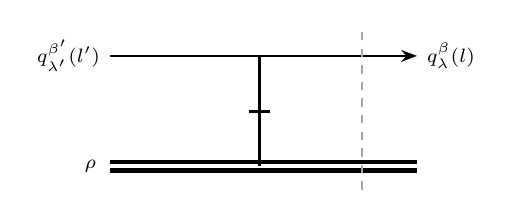
\begin{tikzpicture}
\draw[val] (0,0) -- (3.9,0); \node[left] at (-0.05,0) {\scriptsize$\rho$};
\draw[qk] (0,1.4) -- (3.9,1.4); \node[left] at (0,1.4) {\scriptsize$\qk{\beta'}{\lambda'}{l'}$};
\node[right] at (3.9,1.4) {\scriptsize$\qk{\beta}{\lambda}{l}$};
\draw[ins] (1.9,0) -- (1.9,1.4); \ibar{1.9}{0.7}
\draw[cut] (3.2,-0.3) -- (3.2,1.75);
\end{tikzpicture}
\end{center}
This is the eikonal colour rotation of the soft quark by the $\rho\cdot J_{q}$ term of
\eqref{eq:Hqinst}; with \eqref{eq:MEinstq},
\begin{multline}
\ket{(\Psi^{\beta'}_{\lambda'}(l'))^{3}_{q\,\rho}}=\int\!d^{3}l\;\ket{\qk{\beta}{\lambda}{l}}\,
\frac{\bra{\qk{\beta}{\lambda}{l}}H_{q-{\rm inst}}\ket{\qk{\beta'}{\lambda'}{l'}}}{\Delta}\\
=\frac{g^{2}}{8\pi^{3}}\int\!d^{3}l\;\ket{\qk{\beta}{\lambda}{l}}\,
\frac{t^{b}_{\beta\beta'}\,\rho^{b}(l'-l)\,\delta_{\lambda\lambda'}}{(l'^{+}-l^{+})^{2}\,\Delta} .
\label{eq:P1c}
\end{multline}

\paragraph{(d) Self-energy.} The quark may also emit and reabsorb a soft gluon. This contribution
is proportional to $\dthree(l-l')$, has $E_{i}=E_{f}$, and enters only the normalization,
discussed below.

\paragraph{Simplification.} For $p=l'-l$ the vertex satisfies
\begin{equation}
p^{j}\Gam^{j}(p;l,l')=4\eps_{p}-2\Delta-\frac{p^{+}}{l^{+}l'^{+}}(\bm\sigma\!\cdot\!\bm l)(\bm\sigma\!\cdot\!\bm l'),
\label{eq:pGam1}
\end{equation}
and for $p=l-l'$, $p^{j}\Gam^{j}(p;l,l')=4\eps_{p}+2\Delta-\tfrac{p^{+}}{l^{+}l'^{+}}(\bm\sigma\!\cdot\!\bm l)(\bm\sigma\!\cdot\!\bm l')$.
Writing $4\eps_{p}-2\Delta=-4(\Delta-\eps_{p})+2\Delta$ in \eqref{eq:P1a}, and
$4\eps_{p}+2\Delta$ unchanged in \eqref{eq:P1b}, the terms proportional to
$\delta_{\lambda\lambda'}/\Delta$ cancel the instantaneous contribution \eqref{eq:P1c} in both
kinematic regions, exactly as in the vacuum sector. The sum is
\begin{align}
\ket{(\Psi^{\beta'}_{\lambda'}(l'))_{q\,\rho}}=\;&\frac{g^{2}}{32\pi^{3}}\int\!d^{3}l\;\ket{\qk{\beta}{\lambda}{l}}\,
\frac{t^{b}_{\beta\beta'}\rho^{b}(l'-l)}{(p^{+})^{2}}\,\chi^{\dg}_{\lambda}\Bigg\{
\nonumber\\&\hspace{0.6cm}
\theta(l'^{+}-l^{+})\left[\frac{2}{\Delta-\eps_{p}}
-\frac{p^{+}\,(\bm\sigma\!\cdot\!\bm l)(\bm\sigma\!\cdot\!\bm l')}{l^{+}l'^{+}\,(\Delta-\eps_{p})\,\Delta}\right]
\nonumber\\
&\hspace{0.6cm}-\theta(l^{+}-l'^{+})\left[\frac{2}{\eps_{p}}
-\frac{p^{+}\,(\bm\sigma\!\cdot\!\bm l)(\bm\sigma\!\cdot\!\bm l')}{l^{+}l'^{+}\,\eps_{p}\,\Delta}\right]\Bigg\}\chi_{\lambda'},
\label{eq:Pq-q}
\end{align}
where $p=\pm(l'-l)$ is the (positive plus momentum) gluon exchanged in the two regions. The
overall denominator $\Delta=\eps_{l'}-\eps_{l}$ survives in the helicity dependent term: the
coefficient $\mf P$ has an on-shell pole, exactly as the coefficient $B_{3}$ of Paper~I, and its
residue is the amplitude for the scattering of a soft quark on the valence charge.

\subsubsection{Quark and two gluons outgoing}

At order $g^{2}$ the transition $q(l')\to q(l)\,\gl{c}{k}{q}\gl{d}{n}{r}$ receives five
contributions:
\begin{center}
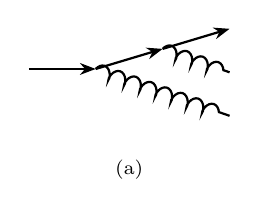
\begin{tikzpicture}[scale=0.85]
\draw[qk] (0,1.2) -- (1.0,1.2); \draw[qk] (1.0,1.2) -- (2.0,1.5); \draw[qk] (2.0,1.5) -- (3.0,1.8);
\draw[gl] (1.0,1.2) -- (3.0,0.5); \draw[gl] (2.0,1.5) -- (3.0,1.15);
\node at (1.5,-0.3) {\scriptsize (a)};
\end{tikzpicture}\hspace{0.35cm}
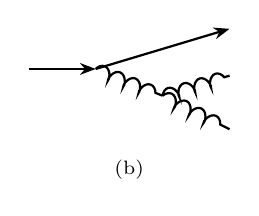
\begin{tikzpicture}[scale=0.85]
\draw[qk] (0,1.2) -- (1.0,1.2); \draw[qk] (1.0,1.2) -- (3.0,1.8);
\draw[gl] (1.0,1.2) -- (2.0,0.8); \draw[gl] (2.0,0.8) -- (3.0,1.1); \draw[gl] (2.0,0.8) -- (3.0,0.3);
\node at (1.5,-0.3) {\scriptsize (b)};
\end{tikzpicture}\hspace{0.35cm}
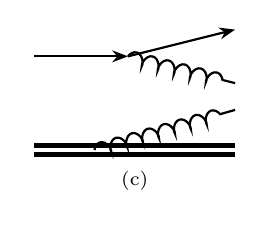
\begin{tikzpicture}[scale=0.85]
\draw[val] (0,0) -- (3.0,0);
\draw[qk] (0,1.4) -- (1.4,1.4); \draw[qk] (1.4,1.4) -- (3.0,1.8);
\draw[gl] (1.4,1.4) -- (3.0,1.0); \draw[gl] (0.9,0) -- (3.0,0.6);
\node at (1.5,-0.45) {\scriptsize (c)};
\end{tikzpicture}\hspace{0.35cm}
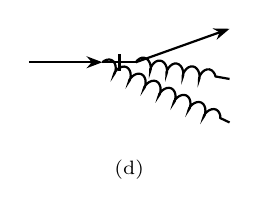
\begin{tikzpicture}[scale=0.85]
\draw[qk] (0,1.3) -- (1.1,1.3); \draw[qk] (1.6,1.3) -- (3.0,1.8);
\draw[ins] (1.1,1.3) -- (1.6,1.3); \ibarh{1.35}{1.3}
\draw[gl] (1.1,1.3) -- (3.0,0.4); \draw[gl] (1.6,1.3) -- (3.0,1.05);
\node at (1.5,-0.3) {\scriptsize (d)};
\end{tikzpicture}\hspace{0.35cm}
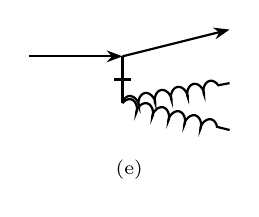
\begin{tikzpicture}[scale=0.85]
\draw[qk] (0,1.4) -- (1.4,1.4); \draw[qk] (1.4,1.4) -- (3.0,1.8);
\draw[ins] (1.4,1.4) -- (1.4,0.7); \ibar{1.4}{1.05}
\draw[gl] (1.4,0.7) -- (3.0,1.0); \draw[gl] (1.4,0.7) -- (3.0,0.3);
\node at (1.5,-0.3) {\scriptsize (e)};
\end{tikzpicture}
\end{center}
(a) two sequential emissions by the quark, in either order; (b) emission of a gluon which splits
into two through $H_{ggg}$; (c) emission of one gluon by the quark and of the other by the
valence charge; (d) instantaneous quark exchange; (e) instantaneous gluon exchange between the
quark and gluon currents. With $D_{f}=\eps_{l'}-\eps_{l}-\eps_{q}-\eps_{r}$,
\begin{align}
\ket{(\Psi^{\beta'}_{\lambda'}(l'))_{qgg}}=\;&\frac12\int\!d^{3}l\,d^{3}q\,d^{3}r\;\ket{\qk{\beta}{\lambda}{l}\gl{c}{k}{q}\gl{d}{n}{r}}
\nonumber\\&\times\Bigg\{\int\!d^{3}l_{1}\,\frac{\bra{\qk{\beta}{\lambda}{l}\gl{c}{k}{q}}H_{gq\bar q}\ket{q(l_{1})}}{D_{f}}\,
\frac{\bra{q(l_{1})\gl{d}{n}{r}}H_{gq\bar q}\ket{\qk{\beta'}{\lambda'}{l'}}}{\eps_{l'}-\eps_{l_{1}}-\eps_{r}}
+(q\leftrightarrow r)
\nonumber\\
&+\int\!d^{3}s\,\frac{\bra{\gl{c}{k}{q}\gl{d}{n}{r}}H_{ggg}\ket{g(s)}}{D_{f}}\,
\frac{\bra{\qk{\beta}{\lambda}{l}g(s)}H_{gq\bar q}\ket{\qk{\beta'}{\lambda'}{l'}}}{\eps_{l'}-\eps_{l}-\eps_{s}}
\nonumber\\
&+\frac{\bra{q\,gg}\big(H_{ggq\bar q}+H_{q-{\rm inst}}\big)\ket{q}}{D_{f}}\Bigg\}
\nonumber\\
&+\ket{(\Psi^{\beta'}_{\lambda'}(l'))_{qgg\,\rho}} ,
\label{eq:Pq-qgg}
\end{align}
where the factor $\tfrac12$ compensates the double counting of the identical gluons, the
instantaneous matrix elements are \eqref{eq:MEq2g} and \eqref{eq:MEJJq2g}, and the $\rho$ dependent
component (c) factorizes by \eqref{eq:factor} into the product of \eqref{eq:Pq-qg} and the
Weizs\"acker--Williams amplitude. The diagrams (a)--(e) are related by crossing to the diagrams
(a)--(g) of the $q\bar q g$ component of the one gluon state.

\subsubsection{Quark and a quark--antiquark pair outgoing}

At order $g^{2}$ the quark can also emit a gluon which splits into a pair, or create a pair
through the instantaneous $J_{q}\cdot J_{q}$ interaction:
\begin{center}
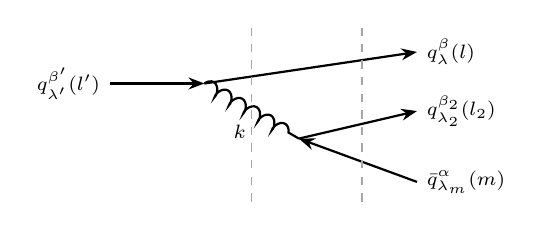
\begin{tikzpicture}
\draw[qk] (0,1.6) -- (1.2,1.6); \node[left] at (0,1.6) {\scriptsize$\qk{\beta'}{\lambda'}{l'}$};
\draw[qk] (1.2,1.6) -- (3.9,2.0); \node[right] at (3.9,2.0) {\scriptsize$\qk{\beta}{\lambda}{l}$};
\draw[gl] (1.2,1.6) -- (2.4,0.9); \node[below left] at (1.85,1.2) {\scriptsize$k$};
\draw[qk] (2.4,0.9) -- (3.9,1.25); \node[right] at (3.9,1.25) {\scriptsize$\qk{\beta_{2}}{\lambda_{2}}{l_{2}}$};
\draw[qk] (3.9,0.35) -- (2.4,0.9); \node[right] at (3.9,0.35) {\scriptsize$\aqk{\alpha}{\lambda_{m}}{m}$};
\draw[cut] (1.8,0.1) -- (1.8,2.3); \draw[cut] (3.2,0.1) -- (3.2,2.3);
\end{tikzpicture}
\hspace{0.8cm}
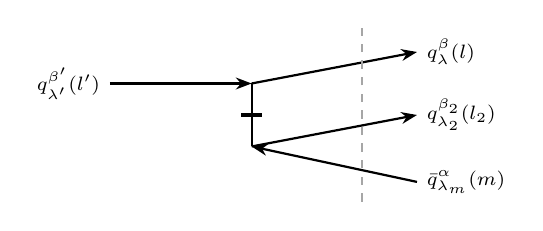
\begin{tikzpicture}
\draw[qk] (0,1.6) -- (1.8,1.6); \node[left] at (0,1.6) {\scriptsize$\qk{\beta'}{\lambda'}{l'}$};
\draw[qk] (1.8,1.6) -- (3.9,2.0); \node[right] at (3.9,2.0) {\scriptsize$\qk{\beta}{\lambda}{l}$};
\draw[ins] (1.8,1.6) -- (1.8,0.8); \ibar{1.8}{1.2}
\draw[qk] (1.8,0.8) -- (3.9,1.2); \node[right] at (3.9,1.2) {\scriptsize$\qk{\beta_{2}}{\lambda_{2}}{l_{2}}$};
\draw[qk] (3.9,0.35) -- (1.8,0.8); \node[right] at (3.9,0.35) {\scriptsize$\aqk{\alpha}{\lambda_{m}}{m}$};
\draw[cut] (3.2,0.1) -- (3.2,2.3);
\end{tikzpicture}
\end{center}
\begin{align}
\ket{(\Psi^{\beta'}_{\lambda'}(l'))_{qq\bar q}}=\;&\frac12\int\!d^{3}l\,d^{3}l_{2}\,d^{3}m\;\ket{\qk{\beta}{\lambda}{l}\qk{\beta_{2}}{\lambda_{2}}{l_{2}}\aqk{\alpha}{\lambda_{m}}{m}}
\nonumber\\&\times\Bigg\{\int\!d^{3}k\,
\frac{\bra{q(l_{2})\bar q(m)}H_{gq\bar q}\ket{g(k)}\bra{q(l)g(k)}H_{gq\bar q}\ket{q(l')}}{D_{f}\,\big(\eps_{l'}-\eps_{l}-\eps_{k}\big)}
\nonumber\\
&+\frac{\bra{q(l)q(l_{2})\bar q(m)}H_{q-{\rm inst}}\ket{q(l')}}{D_{f}}\Bigg\}
\nonumber\\&-\big((\beta,\lambda,l)\leftrightarrow(\beta_{2},\lambda_{2},l_{2})\big),
\label{eq:Pq-qqq}
\end{align}
with $D_{f}=\eps_{l'}-\eps_{l}-\eps_{l_{2}}-\eps_{m}$ and the matrix element \eqref{eq:MEJJqqq}. The
antisymmetrization accounts for the two identical quarks in the final state. The
$\rho$ dependent pair creation off the valence charge with a spectator quark is the
disconnected $\mf A_{1}$ term.

\subsubsection{Single-antiquark incoming state}

The antiquark sector follows from the quark sector by the replacements dictated by the
antiquark vertex \eqref{eq:MEaqg}: the colour matrix is replaced by
$t^{b}_{\beta\beta'}\to-t^{b}_{\alpha'\alpha}$ (incoming colour index first), and the spinor
bilinear of the quark line by that of the antiquark line, in which the incoming helicity stands
on the left, $\Ph^{j}_{\lambda\lambda'}(p;l,l')\to\Ph^{j}_{\lambda'\lambda}(p;m',m)$. For an incoming
antiquark $\ket{\aqk{\alpha'}{\lambda'}{m'}}$ and outgoing $\aqk{\alpha}{\lambda}{m}$ one finds
\begin{align}
\ket{(\Psi^{\alpha'}_{\lambda'}(m'))_{\bar qg}}&=-\frac{g}{8\pi^{3/2}}\int\!d^{3}m\,d^{3}p\;\ket{\bar q g}\,
\frac{t^{b}_{\alpha'\alpha}\,\dthree(m'-m-p)\,\Ph^{j}_{\lambda'\lambda}(p;m',m)}{\sqrt{p^{+}}\,\big(\eps_{m'}-\eps_{m}-\eps_{p}\big)},
\label{eq:Pqb-qbg}\\
\ket{(\Psi^{\alpha'}_{\lambda'}(m'))_{\bar q\,\rho}}&=-\frac{g^{2}}{32\pi^{3}}\int\!d^{3}m\;\ket{\aqk{\alpha}{\lambda}{m}}\,
\frac{t^{b}_{\alpha'\alpha}\rho^{b}(m'-m)}{(p^{+})^{2}}\,\chi^{\dg}_{\lambda'}\Bigg\{
\nonumber\\&\hspace{1.0cm}
\theta(m'^{+}-m^{+})\left[\frac{2}{\bar\Delta-\eps_{p}}
-\frac{p^{+}(\bm\sigma\!\cdot\!\bm m')(\bm\sigma\!\cdot\!\bm m)}{m^{+}m'^{+}(\bar\Delta-\eps_{p})\bar\Delta}\right]
\nonumber\\
&\hspace{1.0cm}-\theta(m^{+}-m'^{+})\left[\frac{2}{\eps_{p}}
-\frac{p^{+}(\bm\sigma\!\cdot\!\bm m')(\bm\sigma\!\cdot\!\bm m)}{m^{+}m'^{+}\eps_{p}\bar\Delta}\right]\Bigg\}\chi_{\lambda},
\label{eq:Pqb-qb}
\end{align}
with $\bar\Delta=\eps_{m'}-\eps_{m}$ and $p=\pm(m'-m)$. We have verified \eqref{eq:Pqb-qb}
explicitly: the cancellation of the instantaneous term proceeds as for the quark, with the
instantaneous matrix element \eqref{eq:MEinstqb} carrying the antiquark charge.

\subsubsection{Summary of results}
\label{sec:sum-q}

The dressed quark state through $\order{g^{2}}$ is
\begin{multline}
\ket{\Psi^{\beta'}_{\lambda'}(l')}=N\ket{\qk{\beta'}{\lambda'}{l'}}
+\ket{(\Psi^{\beta'}_{\lambda'}(l'))_{qg}}+\ket{\qk{\beta'}{\lambda'}{l'}}\otimes\ket{\Psi^{\rm LO}_{g\,\rho}}\\
+\ket{(\Psi^{\beta'}_{\lambda'}(l'))_{q\,\rho}}+\ket{(\Psi^{\beta'}_{\lambda'}(l'))_{qgg}}
+\ket{(\Psi^{\beta'}_{\lambda'}(l'))_{qq\bar q}}+\dots,
\label{eq:sum-q}
\end{multline}
where $\ket{\Psi^{\rm LO}_{g\,\rho}}$ is the leading order Weizs\"acker--Williams component of the
vacuum and the dots denote the remaining disconnected components (the order $g^{2}$ vacuum
components with the quark as a spectator). As in the gluon case, the normalization is fixed by
$\langle\Psi|\Psi\rangle=1$. The $\rho$ dependent overlaps reproduce those of the vacuum, and the
only new contribution is the norm of the $qg$ component. With $z=p^{+}/l'^{+}$ and
$\bm\kappa=\bm p-z\bm l'$ of \eqref{eq:kappaq}, for fixed $\lambda'$,
\begin{equation}
\sum_{\lambda,j}\big|\Ph^{j}_{\lambda\lambda'}(p;l,l')\big|^{2}
=\frac{2\,\bm\kappa^{2}\big[1+(1-z)^{2}\big]}{(l'^{+})^{2}z^{2}(1-z)^{2}},
\end{equation}
and
\begin{multline}
\big\langle(\Psi^{\beta''}_{\lambda''}(l''))_{qg}\big|(\Psi^{\beta'}_{\lambda'}(l'))_{qg}\big\rangle
=\delta^{\beta'\beta''}\delta_{\lambda'\lambda''}\dthree(l'-l'')\,\frac{g^{2}C_{F}}{8\pi^{3}}
\int_{\Lambda/l'^{+}}^{1}\!dz\;\frac{1+(1-z)^{2}}{z}\int\!\frac{d^{2}\kappa}{\bm\kappa^{2}}\\
=\delta\delta\delta\;\frac{g^{2}C_{F}}{8\pi^{3}}\Big[2\log\frac{l'^{+}}{\Lambda}-\frac32\Big]\int\!\frac{d^{2}\kappa}{\bm\kappa^{2}} .
\label{eq:qnorm}
\end{multline}
The longitudinal integral contains the soft gluon logarithm, and the transverse integral is
scaleless and vanishes in dimensional regularization. The normalization of the quark state is
therefore the same $N$ as for all the other sectors, as it must be since $\OM$ is a single
operator.

%----------------------------------------------------------------------
\subsection{Calculation of the quark--antiquark incoming state}
\label{sec:wf-qq}
%----------------------------------------------------------------------

For an incoming pair $\ket{\qk{\beta'}{\lambda_{1}'}{l'}\aqk{\alpha'}{\lambda_{2}'}{m'}}$ the possible
final configurations are the vacuum, one gluon, two gluons, a pair with one gluon and a pair. The
first three test the unitarity relations of the coefficients that annihilate pairs; the last
fixes $\mf D_{3}$.

\subsubsection{Vacuum, one and two gluons outgoing}

At order $g$ the pair annihilates into a gluon:
\begin{multline}
\ket{(\Psi(l',m'))_{g}}=\int\!d^{3}k\;\ket{\gl{a}{i}{k}}\,
\frac{\bra{\gl{a}{i}{k}}H_{gq\bar q}\ket{q\bar q}}{\eps_{l'}+\eps_{m'}-\eps_{k}}\\
=-\frac{g}{8\pi^{3/2}}\int\!d^{3}k\;\ket{\gl{a}{i}{k}}\,
\frac{t^{a}_{\alpha'\beta'}\,\dthree(k-l'-m')\,\big[\Ph^{i}_{\lambda_{1}'\lambda_{2}'}(k;l',m')\big]^{*}}
{\sqrt{k^{+}}\,\big(\eps_{k}-\eps_{l'}-\eps_{m'}\big)} .
\label{eq:Pqq-g}
\end{multline}
Comparing with \eqref{eq:Pg} and \eqref{eq:Omqq} one reads off
$\mf A_{4}=-\mf A_{3}^{\dg}$, which is the first relation of \eqref{eq:U1}; the minus sign is the
sign of the energy denominator. At order $g^{2}$ the pair annihilates into the gluon which is
absorbed by the valence, or annihilates instantaneously on $\rho$. By the reduction formula
\eqref{eq:reduction}, the first is $(-A^{\dg})\mf A_{4}\,\eps_{k}/(\eps_{l'}+\eps_{m'})$ and the second
is the Hermitian conjugate of \eqref{eq:Pvac2} with the opposite sign of the energy
denominator. Their sum reproduces \eqref{eq:UA2} exactly: the instantaneous terms are
anti-Hermitian and cancel between $\mf A_{1}$ and $\mf A_{2}^{\dg}$, while
$-\mf A_{1}^{\dg}+A^{\dg}\mf A_{3}^{\dg}=A^{\dg}\mf A_{3}^{\dg}\,\eps_{k}/(\eps_{l'}+\eps_{m'})+\dots$.
Similarly, the transition $q\bar q\to gg$ computed in LCPT (the time reversed diagrams of
section~\ref{sec:wf-gg}) reproduces the relation \eqref{eq:UB2}, including the terms with $\mf F$
and $\mf G$ which arise from the $t$- and $u$-channel exchanges.

\subsubsection{Quark--antiquark outgoing}

The overall energy denominator is
\begin{equation}
D_{f}\equiv\eps_{l'}+\eps_{m'}-\eps_{l}-\eps_{m}.
\end{equation}
Five connected diagrams contribute at order $g^{2}$.

\paragraph{(a) $s$-channel: the pair annihilates into a gluon which splits again.}
\begin{center}
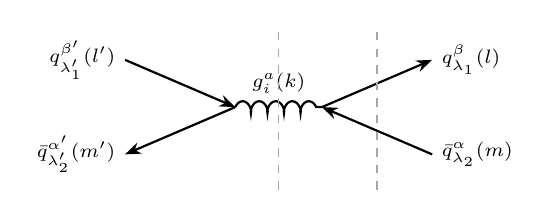
\begin{tikzpicture}
\draw[qk] (0,1.85) -- (1.4,1.25); \node[left] at (0,1.85) {\scriptsize$\qk{\beta'}{\lambda_{1}'}{l'}$};
\draw[qk] (1.4,1.25) -- (0,0.65); \node[left] at (0,0.65) {\scriptsize$\aqk{\alpha'}{\lambda_{2}'}{m'}$};
\draw[gl] (1.4,1.25) -- (2.5,1.25); \node[above] at (1.95,1.3) {\scriptsize$\gl{a}{i}{k}$};
\draw[qk] (2.5,1.25) -- (3.9,1.85); \node[right] at (3.9,1.85) {\scriptsize$\qk{\beta}{\lambda_{1}}{l}$};
\draw[qk] (3.9,0.65) -- (2.5,1.25); \node[right] at (3.9,0.65) {\scriptsize$\aqk{\alpha}{\lambda_{2}}{m}$};
\draw[cut] (1.95,0.2) -- (1.95,2.25); \draw[cut] (3.2,0.2) -- (3.2,2.25);
\end{tikzpicture}
\end{center}
\begin{equation}
\ket{(\Psi(l',m'))^{1}_{q\bar q}}=\int\! d^{3}k\,d^{3}l\,d^{3}m\;\ket{q\bar q}\;
\frac{\bra{q\bar q}H_{gq\bar q}\ket{\gl{a}{i}{k}}}{D_{f}}\;
\frac{\bra{\gl{a}{i}{k}}H_{gq\bar q}\ket{\qk{\beta'}{\lambda_{1}'}{l'}\aqk{\alpha'}{\lambda_{2}'}{m'}}}
{\eps_{l'}+\eps_{m'}-\eps_{k}} .
\end{equation}
With $(t^{a}_{\beta'\alpha'})^{*}=t^{a}_{\alpha'\beta'}$ and $k=l+m=l'+m'$,
\begin{multline}
\ket{(\Psi(l',m'))^{1}_{q\bar q}}=\frac{g^{2}}{64\pi^{3}}\int\!d^{3}l\,d^{3}m\;\ket{q\bar q}\;
\\
\times t^{a}_{\beta\alpha}t^{a}_{\alpha'\beta'}\;\dthree(l+m-l'-m')\,
\frac{\Ph^{i}_{\lambda_{1}\lambda_{2}}(k;l,m)\,
\big[\Ph^{i}_{\lambda_{1}'\lambda_{2}'}(k;l',m')\big]^{*}}
{k^{+}\,\big(\eps_{l'}+\eps_{m'}-\eps_{k}\big)\,D_{f}} .
\label{eq:D3a}
\end{multline}

\paragraph{(b), (c) $t$-channel gluon exchange.}
\begin{center}
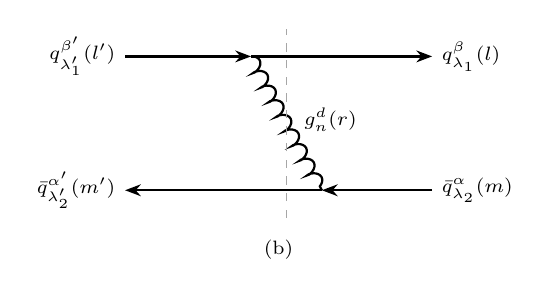
\begin{tikzpicture}
\draw[qk] (0,2.0) -- (1.6,2.0); \node[left] at (0,2.0) {\scriptsize$\qk{\beta'}{\lambda_{1}'}{l'}$};
\draw[qk] (1.6,2.0) -- (3.9,2.0); \node[right] at (3.9,2.0) {\scriptsize$\qk{\beta}{\lambda_{1}}{l}$};
\draw[qk] (3.9,0.3) -- (2.5,0.3); \node[right] at (3.9,0.3) {\scriptsize$\aqk{\alpha}{\lambda_{2}}{m}$};
\draw[qk] (2.5,0.3) -- (0,0.3); \node[left] at (0,0.3) {\scriptsize$\aqk{\alpha'}{\lambda_{2}'}{m'}$};
\draw[gl] (1.6,2.0) -- (2.5,0.3); \node[right] at (2.15,1.2) {\scriptsize$\gl{d}{n}{r}$};
\draw[cut] (2.05,-0.05) -- (2.05,2.35);
\node at (1.95,-0.45) {\scriptsize (b)};
\end{tikzpicture}
\hspace{0.8cm}
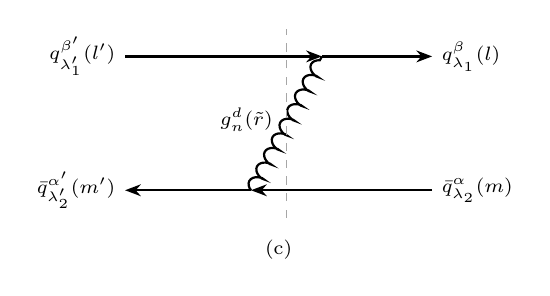
\begin{tikzpicture}
\draw[qk] (0,2.0) -- (2.5,2.0); \node[left] at (0,2.0) {\scriptsize$\qk{\beta'}{\lambda_{1}'}{l'}$};
\draw[qk] (2.5,2.0) -- (3.9,2.0); \node[right] at (3.9,2.0) {\scriptsize$\qk{\beta}{\lambda_{1}}{l}$};
\draw[qk] (3.9,0.3) -- (1.6,0.3); \node[right] at (3.9,0.3) {\scriptsize$\aqk{\alpha}{\lambda_{2}}{m}$};
\draw[qk] (1.6,0.3) -- (0,0.3); \node[left] at (0,0.3) {\scriptsize$\aqk{\alpha'}{\lambda_{2}'}{m'}$};
\draw[gl] (1.6,0.3) -- (2.5,2.0); \node[left] at (2.0,1.2) {\scriptsize$\gl{d}{n}{\tilde r}$};
\draw[cut] (2.05,-0.05) -- (2.05,2.35);
\node at (1.95,-0.45) {\scriptsize (c)};
\end{tikzpicture}
\end{center}
In (b) the quark emits the gluon $r=l'-l$ (so that $l'^{+}>l^{+}$) which the antiquark absorbs;
in (c) the antiquark emits $\tilde r=m'-m$ (so that $m'^{+}>m^{+}$) which the quark absorbs.
Using \eqref{eq:MEqg}, \eqref{eq:MEaqg} and their conjugates,
\begin{align}
\ket{(\Psi(l',m'))^{2}_{q\bar q}}&=-\frac{g^{2}}{64\pi^{3}}\int\!d^{3}l\,d^{3}m\;\ket{q\bar q}\;
t^{d}_{\beta\beta'}t^{d}_{\alpha'\alpha}\;\dthree(l+m-l'-m')
\nonumber\\&\hspace{3cm}\times
\frac{\Ph^{n}_{\lambda_{1}\lambda_{1}'}(r;l,l')\,\Ph^{n}_{\lambda_{2}'\lambda_{2}}(r;m',m)}
{r^{+}\,\big(\eps_{l'}-\eps_{l}-\eps_{r}\big)\,D_{f}}\,\theta(r^{+}),
\label{eq:D3b}\\
\ket{(\Psi(l',m'))^{3}_{q\bar q}}&=-\frac{g^{2}}{64\pi^{3}}\int\!d^{3}l\,d^{3}m\;\ket{q\bar q}\;
t^{d}_{\beta\beta'}t^{d}_{\alpha'\alpha}\;\dthree(l+m-l'-m')
\nonumber\\&\hspace{3cm}\times
\frac{\Ph^{n}_{\lambda_{1}\lambda_{1}'}(\tilde r;l,l')\,\Ph^{n}_{\lambda_{2}'\lambda_{2}}(\tilde r;m',m)}
{\tilde r^{+}\,\big(\eps_{m'}-\eps_{m}-\eps_{\tilde r}\big)\,D_{f}}\,\theta(\tilde r^{+}) .
\label{eq:D3c}
\end{align}
The two orderings populate the complementary regions $l'^{+}\gtrless l^{+}$.

\paragraph{(d) Instantaneous gluon exchange between the quark and the antiquark.}
\begin{center}
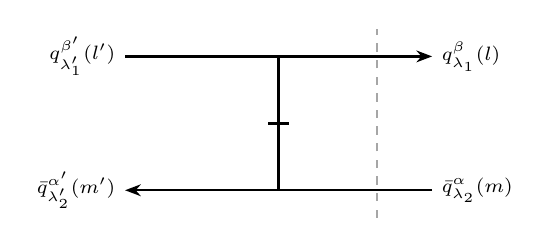
\begin{tikzpicture}
\draw[qk] (0,2.0) -- (3.9,2.0); \node[left] at (0,2.0) {\scriptsize$\qk{\beta'}{\lambda_{1}'}{l'}$};
\node[right] at (3.9,2.0) {\scriptsize$\qk{\beta}{\lambda_{1}}{l}$};
\draw[qk] (3.9,0.3) -- (0,0.3); \node[left] at (0,0.3) {\scriptsize$\aqk{\alpha'}{\lambda_{2}'}{m'}$};
\node[right] at (3.9,0.3) {\scriptsize$\aqk{\alpha}{\lambda_{2}}{m}$};
\draw[ins] (1.95,2.0) -- (1.95,0.3); \ibar{1.95}{1.15}
\draw[cut] (3.2,-0.05) -- (3.2,2.35);
\end{tikzpicture}
\end{center}
This is the $J_{q}\cdot J_{q}$ term of \eqref{eq:Hqinst}; the exchanged line carries
$P^{+}=l'^{+}-l^{+}$ and the antiquark charge supplies a minus sign:
\begin{equation}
\ket{(\Psi(l',m'))^{4}_{q\bar q}}=-\frac{g^{2}}{(2\pi)^{3}}\int\!d^{3}l\,d^{3}m\;\ket{q\bar q}\;
\frac{t^{a}_{\beta\beta'}t^{a}_{\alpha'\alpha}\,\delta_{\lambda_{1}\lambda_{1}'}\delta_{\lambda_{2}\lambda_{2}'}\,
\dthree(l+m-l'-m')}{(l'^{+}-l^{+})^{2}\;D_{f}} .
\label{eq:D3d}
\end{equation}
The diagrams (b), (c) and (d) together build the full $t$-channel one-gluon exchange between the
quark and the antiquark in light-cone gauge.

\paragraph{(e) Instantaneous $s$-channel gluon exchange.}
\begin{center}
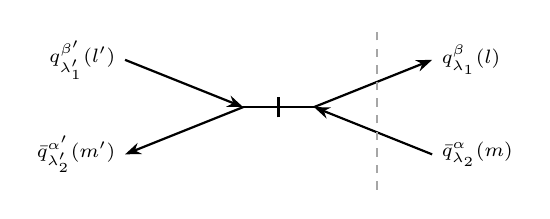
\begin{tikzpicture}
\draw[qk] (0,1.85) -- (1.5,1.25); \node[left] at (0,1.85) {\scriptsize$\qk{\beta'}{\lambda_{1}'}{l'}$};
\draw[qk] (1.5,1.25) -- (0,0.65); \node[left] at (0,0.65) {\scriptsize$\aqk{\alpha'}{\lambda_{2}'}{m'}$};
\draw[ins] (1.5,1.25) -- (2.4,1.25); \ibarh{1.95}{1.25}
\draw[qk] (2.4,1.25) -- (3.9,1.85); \node[right] at (3.9,1.85) {\scriptsize$\qk{\beta}{\lambda_{1}}{l}$};
\draw[qk] (3.9,0.65) -- (2.4,1.25); \node[right] at (3.9,0.65) {\scriptsize$\aqk{\alpha}{\lambda_{2}}{m}$};
\draw[cut] (3.2,0.2) -- (3.2,2.25);
\end{tikzpicture}
\end{center}
The $J_{q}\cdot J_{q}$ interaction also annihilates the incoming pair and creates the outgoing one
instantaneously; the exchanged line carries $P^{+}=k^{+}=l^{+}+m^{+}$:
\begin{equation}
\ket{(\Psi(l',m'))^{5}_{q\bar q}}=\frac{g^{2}}{(2\pi)^{3}}\int\!d^{3}l\,d^{3}m\;\ket{q\bar q}\;
\frac{t^{a}_{\beta\alpha}t^{a}_{\alpha'\beta'}\,\delta_{\lambda_{1}\lambda_{2}}\delta_{\lambda_{1}'\lambda_{2}'}\,
\dthree(l+m-l'-m')}{(k^{+})^{2}\;D_{f}} .
\label{eq:D3e}
\end{equation}
It is the instantaneous part of the $s$-channel exchange (a), in the same way as (d) is that of
(b), (c).

\paragraph{Disconnected contributions.} The exchange of a gluon between the quark (or antiquark)
and the valence charge, with the other member of the pair a spectator, is the coefficient
$\mf P$ ($\bar{\mf P}$) of \eqref{eq:Omqq} computed in section~\ref{sec:wf-q}; it is not part of
$\mf D_{3}$.

\subsubsection{Summary of results}
\label{sec:sum-qq}

The connected $q\bar q\to q\bar q$ amplitude at order $g^{2}$ is the sum of \eqref{eq:D3a}--\eqref{eq:D3e};
its overall denominator $D_{f}$ vanishes on the energy shell and is understood with the
prescription of section~\ref{sec:lcpt}. The remaining components of the dressed pair state are
products of the single quark and single antiquark components and of the order $g$ annihilation
amplitude \eqref{eq:Pqq-g}.

%----------------------------------------------------------------------
\subsection{Calculation of the quark--gluon incoming state}
\label{sec:wf-qg}
%----------------------------------------------------------------------

Finally, for an incoming state $\ket{\qk{\beta'}{\lambda'}{l'}\gl{c}{k}{q}}$ the connected order
$g^{2}$ transition into $\ket{\qk{\beta}{\lambda}{l}\gl{d}{n}{r}}$ is soft quark--gluon (Compton)
scattering. The light-cone time ordered contributions are: the $s$-channel (the quark absorbs
the gluon and re-emits one); the $u$-channel in its two orderings (the quark first emits the
gluon $r$ and then absorbs $q$, or the gluon $q$ first splits into a pair whose antiquark
annihilates with the incoming quark into the gluon $r$); the $t$-channel in its two orderings (the
gluon $q$ splits into two gluons one of which is absorbed by the quark, or the quark emits a gluon
which merges with $q$); the instantaneous quark exchange; and the instantaneous $J_{q}\cdot J_{g}$
gluon exchange. In addition there are the $\rho$ dependent products in which the incoming gluon is
absorbed by the valence while the quark emits the outgoing gluon, or the valence emits the outgoing
gluon while the quark absorbs the incoming one; by \eqref{eq:factor} these factorize. With the
reduction formula \eqref{eq:reduction}, each contribution is the product of two of the first order
amplitudes already computed, weighted by the corresponding ratio of energy denominators, or an
instantaneous matrix element divided by $D_{f}=\eps_{l'}+\eps_{q}-\eps_{l}-\eps_{r}$. The resulting
coefficient $\mf Q_{2}$ is given in section~\ref{sec:coeff}; like $\mf D_{3}$, its $\rho$
independent part has an on-shell pole.

%% ---------------- sec5_coeff.tex ----------------
%======================================================================
\section{Coefficients of the evolution operator up to $\order{g^{2}}$ through LCPT}
\label{sec:coeff}
%======================================================================

To determine the coefficients of the evolution operator we compare its action on the elementary
Fock states, Eqs.~\eqref{eq:Omvac}--\eqref{eq:Omqg}, with the light-cone wave functions computed in
section~\ref{sec:omega}, using the rule \eqref{eq:rule}. Since these states probe different
sectors of Fock space, they constrain different structures of $\OM$, and the coefficients are fixed
one by one. Wherever possible we express the second order coefficients through the first order
ones by the reduction formula \eqref{eq:reduction}, which in terms of coefficients reads: for a
transition $i\to f$ through an intermediate state $m$ generated by the first order structures with
coefficients $X$ ($i\to m$) and $Y$ ($m\to f$),
\begin{equation}
K_{f\leftarrow i}\supset Y\,X\;\frac{E_{m}-E_{f}}{E_{i}-E_{f}},
\qquad\text{and}\qquad
K_{f\leftarrow i}\supset\frac{(2\pi)^{3(n+M)/2}\,H^{(2)}_{fi}}{E_{i}-E_{f}}
\label{eq:redcoef}
\end{equation}
for the instantaneous terms, the internal momenta being integrated with $\int_{p}$. This is the
form in which the coefficients $D_{1}$, $D_{2}$ of Paper~I were written. In the terms that involve the
three-gluon coefficients $C$ and $C_{2}=-C^{\dg}$, the combinatorial factors associated with identical
gluons are those of Paper~I, whose conventions for these coefficients we adopt throughout.

\subsection{Order $g$}

Matching \eqref{eq:Pg}, \eqref{eq:Pq-qg} and \eqref{eq:Pqb-qbg} with \eqref{eq:Omg} and \eqref{eq:Omq}
($K=(2\pi)^{9/2}\psi$) gives
\begin{align}
\mf A^{b\alpha\beta}_{3\,j\lambda_{2}\lambda_{1}}(p,m,l)&=
\frac{(2\pi)^{3}g\,t^{b}_{\beta\alpha}}{2\sqrt2\sqrt{p^{+}}}\;
\frac{\dthree(p-l-m)\;\Ph^{j}_{\lambda_{1}\lambda_{2}}(p;l,m)}{\eps_{p}-\eps_{l}-\eps_{m}},
\label{eq:A3}\\
\mf F^{\beta'\beta b}_{\lambda'\lambda j}(l',l,p)&=
\frac{(2\pi)^{3}g\,t^{b}_{\beta\beta'}}{2\sqrt2\sqrt{p^{+}}}\;
\frac{\dthree(l'-l-p)\;\Ph^{j}_{\lambda\lambda'}(p;l,l')}{\eps_{l'}-\eps_{l}-\eps_{p}},
\label{eq:F}\\
\mf G^{\alpha'\alpha b}_{\lambda'\lambda j}(m',m,p)&=
-\frac{(2\pi)^{3}g\,t^{b}_{\alpha'\alpha}}{2\sqrt2\sqrt{p^{+}}}\;
\frac{\dthree(m'-m-p)\;\Ph^{j}_{\lambda'\lambda}(p;m',m)}{\eps_{m'}-\eps_{m}-\eps_{p}} .
\label{eq:G}
\end{align}
Each of them is the vertex \eqref{eq:V3}--\eqref{eq:VG} divided by the energy released in the
splitting, the quark analogue of the three-gluon coefficient
$C=(2\pi)^{9/2}\bra{gg}H_{ggg}\ket{g}/(E_{i}-E_{f})$ of Paper~I. Their conjugates
$\mf A_{4}$, $\mf F_{2}$, $\mf G_{2}$ follow from \eqref{eq:U1}; for $\mf A_{4}$ this was verified directly
in \eqref{eq:Pqq-g}.

\subsection{Pair creation off the valence charge: $\mf A_{1}$}

Comparing \eqref{eq:Omvac} with \eqref{eq:Pvac} ($K=(2\pi)^{3}\psi$),
\begin{equation}
\boxed{\;
\mf A^{\alpha\beta}_{1\,\lambda_{2}\lambda_{1}}(m,l)=
-g^{2}\,t^{a}_{\beta\alpha}\,\rho^{a}(-k)\left[
\frac{\delta_{\lambda_{1}\lambda_{2}}}{k^{+}\bm k^{2}}
+\frac{\chi^{\dg}_{\lambda_{1}}\big(\bm l\!\cdot\!\bm m+i\,(\bm l\!\times\!\bm m)\,\sigma^{3}\big)\chi_{\lambda_{2}}}
{2\,l^{+}m^{+}\bm k^{2}\,(\eps_{l}+\eps_{m})}\right],\qquad k=l+m,\;}
\label{eq:A1}
\end{equation}
with $\bm l\!\times\!\bm m\equiv\epsilon^{ij}l^{i}m^{j}$. In the form \eqref{eq:redcoef},
$\mf A_{1}=\int_{k}\mf A_{3}(k,m,l)A(k)\,(\eps_{l}+\eps_{m}-\eps_{k})/(\eps_{l}+\eps_{m})
-(2\pi)^{3}\bra{q\bar q}H_{q-{\rm inst}}\vac/(\eps_{l}+\eps_{m})$, with the
Weizs\"acker--Williams coefficient of Paper~I
\begin{equation}
A^{b}_{j}(p)=-\frac{\sqrt2\,g\,p^{j}\rho^{b}(-p)}{\sqrt{p^{+}}\,\bm p^{2}} .
\label{eq:Acoef}
\end{equation}
\emph{Check.} With \eqref{eq:A1}, $\mf A_{1}+\mf A_{2}^{\dg}$ obtained from the direct LCPT
computation of section~\ref{sec:wf-qq} equals $\int_{p}\mf A_{3}(p,m,l)A(p)$, which is the
relation \eqref{eq:UA2}. Using $4(k^{+})^{2}\eps_{k}=2k^{+}\bm k^{2}$, this amounts to the identity
$\frac{1}{2k^{+}\bm k^{2}E}+\frac{1}{4(k^{+})^{2}E(E-\eps_{k})}=\frac{1}{2k^{+}\bm k^{2}(E-\eps_{k})}$
with $E=\eps_{l}+\eps_{m}$; the instantaneous parts cancel.

\subsection{Pair creation off a soft gluon: $\mf B_{3}$}

Comparing \eqref{eq:Omg} with the connected wave functions of section~\ref{sec:wf-g}
($K=(2\pi)^{6}\psi$),
\begin{equation}
\boxed{\;
\mf B^{\alpha\beta ad}_{3\,\lambda_{2}\lambda_{1}in}(m,l,k,r)=A^{d}_{n}(r)\,\mf A^{a\alpha\beta}_{3\,i\lambda_{2}\lambda_{1}}(k,m,l)
+(2\pi)^{6}\Big[\psi^{(1)}+\psi^{(2)}+\psi^{(3)}+\psi^{(6)}+\psi^{(7)}\Big]_{gq\bar q},\;}
\label{eq:B3}
\end{equation}
where $\psi^{(n)}_{gq\bar q}$ denote the coefficient functions of the $q\bar q g$ components
\eqref{eq:B3a}, \eqref{eq:B3b}, \eqref{eq:B3c}, \eqref{eq:B3f} and \eqref{eq:B3g}, i.e.\ the expressions
multiplying $\ket{q\bar q\,g}$ under the integral; their prefactors become $(2\pi)^{3}g^{2}/8$ for
(a), (b), (c) and $(2\pi)^{3}g^{2}/2$ for (f), (g). The first term is the factorized contribution
\eqref{eq:B3de}. Equivalently, by \eqref{eq:redcoef},
\begin{align}
\mf B_{3}(m,l,k,r)=\;&A(r)\mf A_{3}(k,m,l)+\frac{1}{D_{f}}\Big[\int_{p}\mf F(p,l,r)\mf A_{3}(k,m,p)\,(\eps_{p}-\eps_{l}-\eps_{r})
\nonumber\\
&+\int_{m'}\mf G(m',m,r)\mf A_{3}(k,m',l)\,(\eps_{m'}-\eps_{m}-\eps_{r})
\nonumber\\
&+\int_{k'}\mf A_{3}(k',m,l)\,C(k,k',r)\,(\eps_{k'}-\eps_{l}-\eps_{m})
\nonumber\\
&+(2\pi)^{6}\bra{q\bar q\,g}H_{ggq\bar q}+H_{q-{\rm inst}}\ket{g}\Big],
\label{eq:B3red}
\end{align}
with $D_{f}=\eps_{k}-\eps_{l}-\eps_{m}-\eps_{r}$. In each product the weight cancels the energy
denominator of the coefficient that acts second, so that \eqref{eq:B3red} is (vertex)$\times$(first
order coefficient)$/D_{f}$, as in \eqref{eq:B3a}--\eqref{eq:B3c}.

\subsection{Gluon pair annihilation into quarks: $\mf B_{1}$}

The two-gluon state probes the symmetric combination $\mf B_{1}(p,k)+\mf B_{1}(k,p)$,
Eq.~\eqref{eq:Omgg}. Assigning to $\mf B^{ba\alpha\beta}_{1\,ji\lambda_{2}\lambda_{1}}(p,k,m,l)$ the
contributions in which the gluon $\gl{a}{i}{k}$ is absorbed (by the valence charge, by the quark or
by the antiquark) while $\gl{b}{j}{p}$ splits, and half of the contributions that are symmetric by
themselves,
\begin{equation}
\boxed{\;
\begin{aligned}
\mf B^{ba\alpha\beta}_{1\,ji\lambda_{2}\lambda_{1}}(p,k,m,l)=\;&
-A^{\dg a}_{i}(k)\,\mf A^{b\alpha\beta}_{3\,j\lambda_{2}\lambda_{1}}(p,m,l)
\\&+(2\pi)^{6}\Big[\tfrac12\psi^{(1)}+\psi^{(4)}+\psi^{(5)}+\tfrac12\psi^{(6)}+\tfrac12\psi^{(7)}\Big]_{q\bar q},
\end{aligned}\;}
\label{eq:B1}
\end{equation}
where $\psi^{(1)},\psi^{(6)},\psi^{(7)}$ are the coefficient functions of \eqref{eq:B1a}, \eqref{eq:B1e},
\eqref{eq:B1f}, and $\psi^{(4)},\psi^{(5)}$ those of \eqref{eq:B1c}, \eqref{eq:B1d} with
$(a,i,k)\leftrightarrow(b,j,p)$ in the displayed term. The first term is the factorized
contribution \eqref{eq:B1b}. In the form \eqref{eq:redcoef} the $t$- and $u$-channel terms read
\begin{multline}
\mf B_{1}(p,k,m,l)\supset\frac{1}{D_{f}}\Big[\int_{l_{1}}\mf F_{2}(k,l_{1},l)\,\mf A_{3}(p,m,l_{1})\,(\eps_{l_{1}}+\eps_{k}-\eps_{l})
\\+\int_{m_{1}}\mf G_{2}(k,m_{1},m)\,\mf A_{3}(p,m_{1},l)\,(\eps_{m_{1}}+\eps_{k}-\eps_{m})\Big],
\label{eq:B1red}
\end{multline}
which makes manifest that they produce the $\mf F$ and $\mf G$ terms of the unitarity relation
\eqref{eq:UB2}. Since $D_{f}=\eps_{k}+\eps_{p}-\eps_{l}-\eps_{m}$ can vanish, the $\rho$ independent part
of $\mf B_{1}$ has an on-shell pole whose residue is the $gg\to q\bar q$ amplitude.

\subsection{Factorized coefficients: $\mf C_{3}$, $\mf C_{4}$, $\mf D_{1}$}

For these sectors the transition proceeds through two independent subprocesses, the two time
orderings combine by \eqref{eq:factor}, and the coefficients factorize. With
$K=(2\pi)^{9}\psi$ and $(2\pi)^{9}/64\pi^{3}=(2\pi)^{6}/8$, Eqs.~\eqref{eq:Pggqq}, \eqref{eq:Pgqq}
and \eqref{eq:Pqqqq} give
\begin{align}
\mf C^{bcde\alpha\beta}_{4\,jkon\lambda_{2}\lambda_{1}}(p,q,r,s,m,l)&=
\mf A^{b\alpha\beta}_{3\,j\lambda_{2}\lambda_{1}}(p,m,l)\;C^{edc}_{nok}(q,r,s),
\label{eq:C4}\\
\mf C^{bcde\alpha\beta}_{3\,jkon\lambda_{2}\lambda_{1}}(p,q,r,s,m,l)&=
\mf A^{b\alpha\beta}_{3\,j\lambda_{2}\lambda_{1}}(p,m,l)\;C^{edc}_{2\,nok}(q,r,s),
\label{eq:C3}\\
\mf D^{cb\alpha'\beta'\alpha\beta}_{1\,kj\lambda_{2}'\lambda_{1}'\lambda_{2}\lambda_{1}}(q,p,m',l',m,l)&=
\mf A^{b\alpha\beta}_{3\,j\lambda_{2}\lambda_{1}}(p,m,l)\;\mf A^{c\alpha'\beta'}_{3\,k\lambda_{2}'\lambda_{1}'}(q,m',l'),
\label{eq:D1}
\end{align}
where $C$ and $C_{2}=-C^{\dg}$ are the $g\to gg$ and $gg\to g$ coefficients of Paper~I
(Eqs.~(4.8) and (5.5) there). Explicitly, e.g.,
\begin{equation}
\mf C_{4}=\frac{i(2\pi)^{6}g^{2}}{8}\,t^{b}_{\beta\alpha}f^{cde}\,
\frac{\dthree(p-l-m)\dthree(q-r-s)}{\sqrt{p^{+}q^{+}r^{+}s^{+}}}\;
\frac{\Ph^{j}_{\lambda_{1}\lambda_{2}}(p;l,m)\,\Vg^{kon}(q;r,s)}
{\big(\eps_{p}-\eps_{l}-\eps_{m}\big)\big(\eps_{q}-\eps_{r}-\eps_{s}\big)} .
\end{equation}
The factorizations hold with no leftover powers of $2\pi$, which is a stringent check of the
prefactors of $\mf A_{3}$ and of the rule \eqref{eq:rule}. The unitarity partners
$\mf C_{1}$, $\mf C_{2}$, $\mf D_{2}$ follow from \eqref{eq:UC1}--\eqref{eq:UD2}; since $\mf A_{3}$ contains no
$\rho$, two $\mf A_{3}$'s commute and \eqref{eq:UD2} gives
$\mf D_{2}(l,m,l',m',q,p)=\mf A^{\dg}_{3}(q,m,l)\mf A^{\dg}_{3}(p,m',l')$, the crossed assignment, which is
also what a direct LCPT computation of $q\bar q\,q\bar q\to gg$ gives.

\subsection{Quark--antiquark scattering: $\mf D_{3}$}

Comparing \eqref{eq:Omqq} with \eqref{eq:D3a}--\eqref{eq:D3e} ($K=(2\pi)^{6}\psi$; with the ordering
$d\,b$ of \eqref{eq:Om2qq} no extra sign arises),
{\small
\begin{equation}
\boxed{\;
\begin{aligned}
&\mf D^{\beta'\alpha'\alpha\beta}_{3\,\lambda_{1}'\lambda_{2}'\lambda_{2}\lambda_{1}}(l',m',m,l)
=\frac{(2\pi)^{3}g^{2}}{8}\,\frac{\dthree(l+m-l'-m')}{D_{f}}\Bigg\{
\\&\quad
t^{a}_{\beta\alpha}t^{a}_{\alpha'\beta'}\,
\frac{\Ph^{i}_{\lambda_{1}\lambda_{2}}(k;l,m)\,\big[\Ph^{i}_{\lambda_{1}'\lambda_{2}'}(k;l',m')\big]^{*}}
{k^{+}\big(\eps_{l'}+\eps_{m'}-\eps_{k}\big)}
\\
&\quad-t^{d}_{\beta\beta'}t^{d}_{\alpha'\alpha}\Bigg[
\frac{\Ph^{n}_{\lambda_{1}\lambda_{1}'}(r;l,l')\,\Ph^{n}_{\lambda_{2}'\lambda_{2}}(r;m',m)\,\theta(r^{+})}
{r^{+}\big(\eps_{l'}-\eps_{l}-\eps_{r}\big)}
\\&\hspace{2.6cm}+\frac{\Ph^{n}_{\lambda_{1}\lambda_{1}'}(\tilde r;l,l')\,\Ph^{n}_{\lambda_{2}'\lambda_{2}}(\tilde r;m',m)\,\theta(\tilde r^{+})}
{\tilde r^{+}\big(\eps_{m'}-\eps_{m}-\eps_{\tilde r}\big)}\Bigg]
\\
&\quad-\frac{8\,t^{a}_{\beta\beta'}t^{a}_{\alpha'\alpha}\,\delta_{\lambda_{1}\lambda_{1}'}\delta_{\lambda_{2}\lambda_{2}'}}{(l'^{+}-l^{+})^{2}}
+\frac{8\,t^{a}_{\beta\alpha}t^{a}_{\alpha'\beta'}\,\delta_{\lambda_{1}\lambda_{2}}\delta_{\lambda_{1}'\lambda_{2}'}}{(k^{+})^{2}}\Bigg\},
\end{aligned}}
\label{eq:D3}
\end{equation}}
with $k=l+m$, $r=l'-l$, $\tilde r=m'-m$ and $D_{f}=\eps_{l'}+\eps_{m'}-\eps_{l}-\eps_{m}$. In the form
\eqref{eq:redcoef},
\begin{align}
\mf D_{3}(l',m',m,l)=\frac{1}{D_{f}}\Big[&\int_{k}\mf A_{3}(k,m,l)\mf A_{4}(l',m',k)\,(\eps_{k}-\eps_{l}-\eps_{m})
\nonumber\\&+\int_{r}\mf G_{2}(r,m',m)\mf F(l',l,r)\,(\eps_{m'}+\eps_{r}-\eps_{m})
\nonumber\\
&+\int_{\tilde r}\mf F_{2}(\tilde r,l',l)\mf G(m',m,\tilde r)\,(\eps_{l'}+\eps_{\tilde r}-\eps_{l})
\nonumber\\&+(2\pi)^{6}\bra{q\bar q}H_{q-{\rm inst}}\ket{q\bar q}\Big].
\label{eq:D3red}
\end{align}
\emph{Check.} Write $D_{a}=\eps_{k}-\eps_{l}-\eps_{m}$ and $D_{a}'=\eps_{k}-\eps_{l'}-\eps_{m'}$, so that
$D_{a}-D_{a}'=D_{f}$. The $s$-channel term of $\mf D_{3}(l',m',m,l)+\mf D_{3}^{\dg}(l,m,m',l')$ is
\begin{multline}
\frac{(2\pi)^{3}g^{2}}{8}\,\frac{t^{a}t^{a}\,\Ph\Ph^{*}\dthree}{k^{+}}\Big[-\frac{1}{D_{a}'D_{f}}+\frac{1}{D_{a}D_{f}}\Big]
\\=-\frac{(2\pi)^{3}g^{2}}{8}\,\frac{t^{a}t^{a}\,\Ph\Ph^{*}\dthree}{k^{+}D_{a}D_{a}'}
=-\int_{k}\mf A_{3}(k,m,l)\,\mf A_{3}^{\dg}(k,m',l'),
\end{multline}
which is the first term of \eqref{eq:UD3}. In the same way the $t$-channel terms (b) and (c)
reproduce the $\mf F$, $\mf G$ terms of \eqref{eq:UD3}, while the instantaneous term is anti-Hermitian
and drops out. Note that the $t$-channel part of $\mf D_{3}$ is not anti-Hermitian by itself; it
satisfies unitarity only together with the coefficients $\mf F$ and $\mf G$.

\subsection{Quark rescattering on the valence charge: $\mf P$ and $\bar{\mf P}$}

Comparing \eqref{eq:Omq} with \eqref{eq:Pq-q} ($K=(2\pi)^{3}\psi$, $(2\pi)^{3}/32\pi^{3}=1/4$),
\begin{equation}
\boxed{\;
\begin{aligned}
\mf P^{\beta'\beta}_{\lambda'\lambda}(l',l)=\frac{g^{2}}{4}\,\frac{t^{b}_{\beta\beta'}\,\rho^{b}(l'-l)}{(p^{+})^{2}}\,
\chi^{\dg}_{\lambda}\Bigg\{&\theta(l'^{+}-l^{+})\left[\frac{2}{\Delta-\eps_{p}}
-\frac{p^{+}\,(\bm\sigma\!\cdot\!\bm l)(\bm\sigma\!\cdot\!\bm l')}{l^{+}l'^{+}(\Delta-\eps_{p})\,\Delta}\right]
\\
&-\theta(l^{+}-l'^{+})\left[\frac{2}{\eps_{p}}
-\frac{p^{+}\,(\bm\sigma\!\cdot\!\bm l)(\bm\sigma\!\cdot\!\bm l')}{l^{+}l'^{+}\,\eps_{p}\,\Delta}\right]\Bigg\}\chi_{\lambda'},
\end{aligned}}
\label{eq:P}
\end{equation}
with $\Delta=\eps_{l'}-\eps_{l}$ and $p=\pm(l'-l)$ in the two regions. In the form \eqref{eq:redcoef},
\begin{multline}
\mf P(l',l)=-A^{\dg}(p)\,\mf F(l',l,p)\,\frac{\eps_{p}}{\Delta}\Big|_{p=l'-l}
\\-\mf F^{\dg}(l,l',p)\,A(p)\,\frac{\eps_{l'}+\eps_{p}-\eps_{l}}{\Delta}\Big|_{p=l-l'}
+\frac{(2\pi)^{3}\bra{q(l)}H_{q-{\rm inst}}\ket{q(l')}}{\Delta} .
\label{eq:Pred}
\end{multline}
The antiquark coefficient $\bar{\mf P}^{\alpha'\alpha}_{\lambda'\lambda}(m',m)$ is $(2\pi)^{3}$ times the
coefficient function of \eqref{eq:Pqb-qb}.

\emph{Check.} Let $p=l'-l$ with $l'^{+}>l^{+}$. Then $\mf P(l',l)$ is given by the first line of
\eqref{eq:P}, and $\mf P(l,l')$ (incoming $l$, outgoing $l'$) by the second line with $l\leftrightarrow l'$.
Using $\rho^{b}(-p)^{\dg}=\rho^{b}(p)$ and $\big(t^{b}_{\beta'\beta}\big)^{*}=t^{b}_{\beta\beta'}$, and denoting
$S=\chi^{\dg}_{\lambda}(\bm\sigma\!\cdot\!\bm l)(\bm\sigma\!\cdot\!\bm l')\chi_{\lambda'}/(l^{+}l'^{+})$,
\begin{align}
\mf P(l',l)+\mf P^{\dg}(l,l')&=\frac{g^{2}}{4}\frac{t^{b}\rho^{b}(p)}{(p^{+})^{2}}
\Big\{2\delta_{\lambda\lambda'}\Big[\frac{1}{\Delta-\eps_{p}}-\frac{1}{\eps_{p}}\Big]
-p^{+}S\Big[\frac{1}{(\Delta-\eps_{p})\Delta}+\frac{1}{\eps_{p}\Delta}\Big]\Big\}
\nonumber\\
&=\frac{g^{2}}{4}\frac{t^{b}\rho^{b}(p)}{(p^{+})^{2}}\,
\frac{4\eps_{p}-2\Delta-p^{+}S}{(\Delta-\eps_{p})\,\eps_{p}}
\nonumber\\
&=\frac{g^{2}}{4}\frac{t^{b}\rho^{b}(p)\;p^{j}\Ph^{j}_{\lambda\lambda'}(p;l,l')}{(p^{+})^{2}(\Delta-\eps_{p})\,\eps_{p}}
=-\int_{p'}A^{\dg}(p')\,\mf F(l',l,p'),
\end{align}
where we used \eqref{eq:pGam1}, \eqref{eq:Acoef} and \eqref{eq:F}. This is the relation \eqref{eq:UP} (the
self-energy term is momentum diagonal and scaleless). The pole at $\Delta=0$ cancels in the sum, as
it must: $\mf P+\mf P^{\dg}$ is a product of first order coefficients.

\subsection{Coefficients with three outgoing particles: $\mf Q_{1}$, $\mf Q_{2}$, $\mf K_{1}$}

Comparing \eqref{eq:Omq}, \eqref{eq:Omqg} with \eqref{eq:Pq-qgg}, \eqref{eq:Pq-qqq} and with the
quark--gluon amplitude of section~\ref{sec:wf-qg}, and using \eqref{eq:redcoef}, we obtain
\begin{align}
\mf Q_{1}(l',l,q,r)=\frac12\Bigg\{&A(q)\mf F(l',l,r)+A(r)\mf F(l',l,q)
\nonumber\\&+\frac{1}{D_{f}}\Big[\int_{l_{1}}\mf F(l_{1},l,q)\mf F(l',l_{1},r)\,(\eps_{l_{1}}-\eps_{l}-\eps_{q})+(q\leftrightarrow r)
\nonumber\\
&+\int_{s}C(s,q,r)\,\mf F(l',l,s)\,(\eps_{s}-\eps_{q}-\eps_{r})
\nonumber\\&+(2\pi)^{6}\bra{q\,gg}H_{ggq\bar q}+H_{q-{\rm inst}}\ket{q}\Big]\Bigg\},
\label{eq:Q1}
\end{align}
with $D_{f}=\eps_{l'}-\eps_{l}-\eps_{q}-\eps_{r}$;
\begin{align}
\mf K_{1}(l',l,l_{2},m)=\frac12\Bigg\{&\frac{1}{D_{f}}\Big[\int_{k}\mf A_{3}(k,m,l_{2})\,\mf F(l',l,k)\,(\eps_{k}-\eps_{l_{2}}-\eps_{m})
\nonumber\\&+(2\pi)^{6}\bra{q\,q\bar q}H_{q-{\rm inst}}\ket{q}\Big]-\big(l\leftrightarrow l_{2}\big)\Bigg\},
\label{eq:K1}
\end{align}
with $D_{f}=\eps_{l'}-\eps_{l}-\eps_{l_{2}}-\eps_{m}$; and
\begin{align}
\mf Q_{2}(l',q,l,r)=&-A^{\dg}(q)\mf F(l',l,r)+A(r)\mf F_{2}(q,l',l)
\nonumber\\
&+\frac{1}{D_{f}}\Big[\int_{l_{1}}\mf F(l_{1},l,r)\mf F_{2}(q,l',l_{1})\,(\eps_{l_{1}}-\eps_{l}-\eps_{r})
\nonumber\\&\qquad+\int_{l_{1}}\mf F_{2}(q,l_{1},l)\mf F(l',l_{1},r)\,(\eps_{l_{1}}+\eps_{q}-\eps_{l})
\nonumber\\
&\qquad-\int_{m_{1}}\mf A_{4}(l',m_{1},r)\mf A_{3}(q,m_{1},l)\,(\eps_{l'}+\eps_{m_{1}}-\eps_{r})
\nonumber\\&\qquad+\int_{s}\mf F_{2}(s,l',l)\,C(q,s,r)\,(\eps_{s}+\eps_{l'}-\eps_{l})
\nonumber\\
&\qquad+\int_{s}C_{2}(s,q,r)\,\mf F(l',l,s)\,(\eps_{s}+\eps_{q}-\eps_{r})
\nonumber\\&\qquad+(2\pi)^{6}\bra{q\,g}H_{ggq\bar q}+H_{q-{\rm inst}}\ket{q\,g}\Big],
\label{eq:Q2}
\end{align}
with $D_{f}=\eps_{l'}+\eps_{q}-\eps_{l}-\eps_{r}$. The six terms in the bracket of \eqref{eq:Q2} are the
$s$-channel, the two orderings of the $u$-channel (the second, with a soft pair in the intermediate
state, carries the Fermi minus sign) and the two orderings of the $t$-channel, followed by the
instantaneous terms; the first line contains the factorized $\rho$ dependent products. The
instantaneous matrix elements are given in appendix~\ref{app:me}. The antiquark coefficients
$\bar{\mf Q}_{1,2}$, $\bar{\mf K}_{1}$ follow by $\mf F\to\mf G$, $\mf A_{3}\to\mf A_{3}$ with the roles of
quark and antiquark exchanged.

\subsection{Coefficients fixed by unitarity}

The remaining coefficients follow from the constraint equations of section~\ref{sec:omega}:
$\mf A_{4}$, $\mf F_{2}$, $\mf G_{2}$ from \eqref{eq:U1}; $\mf A_{2}$ from \eqref{eq:UA2}; $\mf B_{2}$, $\mf B_{4}$
from \eqref{eq:UB2}, \eqref{eq:UB4}; $\mf C_{1}$, $\mf C_{2}$, $\mf D_{2}$ from \eqref{eq:UC1}--\eqref{eq:UD2};
$\mf Q_{3}$ and $\mf K_{2}$ from \eqref{eq:UQ3}, \eqref{eq:UK2}. Finally, every structure of
$\OM^{(2)}_{\times}$, Eq.~\eqref{eq:Omx}, is the normal ordered product of two first order structures
$X$, $Y$ acting on disjoint particles; by \eqref{eq:factor}, and since at most one of the two
coefficients contains $\rho$,
\begin{equation}
K_{:\hat X\hat Y:}=X\,Y,
\label{eq:Kx}
\end{equation}
e.g.\ the coefficient of $a^{\dg}b^{\dg}d^{\dg}b^{\dg}b\,a$ is $\mf A_{3}\,\mf F$ and that of
$a^{\dg}a^{\dg}b^{\dg}b\,a^{\dg}a$-type structures is $\mf F\,C$. These coefficients satisfy the unitarity
relations identically.

The overall energy denominator $E_{i}-E_{f}$ can vanish only in the coefficients that preserve
the number of soft quarks, antiquarks and gluons, namely $\mf P$, $\bar{\mf P}$, the $\rho$ independent
parts of $\mf D_{3}$ and $\mf Q_{2}$, and in the $2\to2$ coefficients $\mf B_{1}$, $\mf B_{2}$. These are
understood with the prescription of section~\ref{sec:lcpt}, and their residues are on-shell
scattering amplitudes. In all other coefficients the overall denominator either never vanishes
(away from collinear configurations of measure zero) or cancels between the two time orderings,
which then combine into a product of first order coefficients, as in $\mf C_{3}$, $\mf C_{4}$,
$\mf D_{1}$, the factorized parts of $\mf B_{1}$, $\mf B_{3}$, $\mf Q_{1}$, $\mf Q_{2}$, and \eqref{eq:Kx}.

\subsection{The generator}
\label{sec:generator}

Having determined all the coefficients, we reconstruct the evolution operator. As in Paper~I we
write $\OM=e^{iG}$ with $G=G_{\rm YM}+G_{q}$ Hermitian and known through $\order{g^{2}}$. Since
$\OM^{(2)}=iG^{(2)}+\tfrac12(iG^{(1)})^{2}$ and the uncontracted part of $\tfrac12(iG^{(1)})^{2}$ is
$\OM^{(2)}_{\times}$ together with $\mf C_{1,\dots,4}$, $\mf D_{1,2}$ and the factorized parts of the other
coefficients, the connected part of $G_{q}$ is
\begin{align}
G_{q}=&-i\int_{p,l,m}\Big[\mf A_{3}\,b^{\dg}d^{\dg}a-\mf A_{3}^{\dg}\,a^{\dg}db\Big]
-i\int_{p,l,l'}\Big[\mf F\,a^{\dg}b^{\dg}b-\mf F^{\dg}\,b^{\dg}b\,a\Big]
-i\int_{p,m,m'}\Big[\mf G\,a^{\dg}d^{\dg}d-\mf G^{\dg}\,d^{\dg}d\,a\Big]
\nonumber\\
&-\frac{i}{2}\int_{l,m}\Big[\mf A_{1}-\mf A_{2}^{\dg}\Big]b^{\dg}d^{\dg}
-\frac{i}{2}\int_{l,m}\Big[\mf A_{2}-\mf A_{1}^{\dg}\Big]db
-\frac{i}{2}\int_{p,q,l,m}\Big[\mf B_{1}-\mf B_{2}^{\dg}\Big]b^{\dg}d^{\dg}aa
\nonumber\\
&-\frac{i}{2}\int_{p,q,l,m}\Big[\mf B_{2}-\mf B_{1}^{\dg}\Big]a^{\dg}a^{\dg}db
-\frac{i}{2}\int_{p,q,l,m}\Big[\mf B_{3}-\mf B_{4}^{\dg}\Big]a^{\dg}a\,b^{\dg}d^{\dg}
\nonumber\\
&-\frac{i}{2}\int_{p,q,l,m}\Big[\mf B_{4}-\mf B_{3}^{\dg}\Big]db\,a^{\dg}a
\nonumber\\
&-\frac{i}{2}\int_{l,m,l',m'}\Big[\mf D_{3}-\mf D_{3}^{\dg}\Big]b^{\dg}d^{\dg}db
-\frac{i}{2}\int_{l,l'}\Big[\mf P-\mf P^{\dg}\Big]b^{\dg}b
-\frac{i}{2}\int_{m,m'}\Big[\bar{\mf P}-\bar{\mf P}^{\dg}\Big]d^{\dg}d
\nonumber\\
&-\frac{i}{2}\int\Big[\mf Q_{1}-\mf Q_{3}^{\dg}\Big]a^{\dg}a^{\dg}b^{\dg}b
-\frac{i}{2}\int\Big[\mf Q_{3}-\mf Q_{1}^{\dg}\Big]b^{\dg}b\,aa
-\frac{i}{2}\int\Big[\mf Q_{2}-\mf Q_{2}^{\dg}\Big]a^{\dg}b^{\dg}b\,a
\nonumber\\
&-\frac{i}{2}\int\Big[\mf K_{1}-\mf K_{2}^{\dg}\Big]b^{\dg}b^{\dg}d^{\dg}b
-\frac{i}{2}\int\Big[\mf K_{2}-\mf K_{1}^{\dg}\Big]b^{\dg}d\,bb
\nonumber\\
&+\big(q\to\bar q\big),
\label{eq:Gq}
\end{align}
where the arguments and labels are those of \eqref{eq:Om1q}--\eqref{eq:OmF}, $(q\to\bar q)$ denotes the
antiquark analogues of the $\mf Q$ and $\mf K$ terms, and $\mf F$, $\mf G$, $\mf A_{3}$ are of order $g$ while
all the other coefficients are of order $g^{2}$. $G_{q}$ is Hermitian by construction. By the
unitarity relations, each combination $[K-K'^{\dg}]/2$ in \eqref{eq:Gq} equals $K$ minus half of the
corresponding product of first order coefficients; for the particle number preserving coefficients
it is their anti-Hermitian part, which contains the instantaneous terms and the principal value
parts of the on-shell poles.

%% ---------------- sec6_diag.tex ----------------
%======================================================================
\section{Diagonalization of the QCD Hamiltonian at $\order{g}$ and $\order{g^{2}}$}
\label{sec:diag}
%======================================================================

The evolution operator provides a systematic framework for diagonalizing the soft QCD
Hamiltonian of a fast-moving hadron. We use the unitary similarity transformation
\begin{equation}
H\to\OM^{\dg}H\,\OM ,
\label{eq:sim}
\end{equation}
with $\OM$ constructed perturbatively in $g$ with the coefficients fixed in
section~\ref{sec:coeff}. The role of $\OM$ is to cancel the off-diagonal matrix elements of $H$
that connect different Fock sectors, order by order in the coupling. In Paper~I it was shown that
in pure Yang--Mills theory the coherent operator \eqref{eq:coherent} alone is not sufficient: the
three-gluon interaction generates additional structures at the same order. With quarks, the
quark--gluon vertex generates three further structures at order $g$, and all of them must be
included for a complete diagonalization.

Splitting the Hamiltonian by order in the coupling,
\begin{align}
&H=H_{0}+H^{(1)}+H^{(2)},\qquad
H^{(1)}=H_{g}+H_{ggg}+H_{gq\bar q},
\nonumber\\
&H^{(2)}=H_{gggg}+H_{gg-{\rm inst}}+H_{gggg-{\rm inst}}+H_{ggq\bar q}+H_{q-{\rm inst}},
\label{eq:Hsplit}
\end{align}
and using $\OM^{(1)\dg}=-\OM^{(1)}$ and $\OM^{(2)}=iG^{(2)}+\tfrac12\big(\OM^{(1)}\big)^{2}$, one finds
\begin{align}
\OM^{\dg}H\OM\Big|_{g^{1}}&=H^{(1)}+\big[H_{0},\OM^{(1)}\big],
\label{eq:ord1}\\
\OM^{\dg}H\OM\Big|_{g^{2}}&=H^{(2)}+\tfrac12\big[H^{(1)},\OM^{(1)}\big]+\big[H_{0},iG^{(2)}\big],
\label{eq:ord2}
\end{align}
where in \eqref{eq:ord2} we used $\big[[H_{0},\OM^{(1)}],\OM^{(1)}\big]=-[H^{(1)},\OM^{(1)}]$, which
follows once \eqref{eq:ord1} vanishes. For a normal ordered structure $\mathcal O$ whose creation
operators carry total energy $E_{\rm out}$ and whose annihilation operators carry $E_{\rm in}$,
\begin{equation}
\big[H_{0},\mathcal O\big]=\big(E_{\rm out}-E_{\rm in}\big)\,\mathcal O .
\label{eq:H0O}
\end{equation}

\subsection{Order $g$}

Substituting the first order part of the ansatz into \eqref{eq:ord1} and using \eqref{eq:H0O},
\begin{align}
\OM^{\dg}H\OM\Big|_{g^{1}}=&\;H_{g}+H_{ggg}+H_{gq\bar q}
+\int_{p}\Big[A^{b}_{j}(p)\,\eps_{p}\,a^{\dg b}_{j}(p)+A^{\dg b}_{j}(p)\,\eps_{p}\,a^{b}_{j}(p)\Big]
\nonumber\\
&+\int_{p,q,r}\big(\eps_{q}+\eps_{r}-\eps_{p}\big)\Big[C(p,q,r)\,a^{\dg}(r)a^{\dg}(q)a(p)
\nonumber\\&\hspace{4cm}+C^{\dg}(r,q,p)\,a^{\dg}(r)a(q)a(p)\Big]
\nonumber\\
&+\int_{p,l,m}\big(\eps_{l}+\eps_{m}-\eps_{p}\big)\Big[\mf A_{3}(p,m,l)\,b^{\dg}(l)d^{\dg}(m)a(p)
\nonumber\\&\hspace{4cm}+\mf A^{\dg}_{3}(p,m,l)\,a^{\dg}(p)d(m)b(l)\Big]
\nonumber\\
&+\int_{p,l,l'}\big(\eps_{l}+\eps_{p}-\eps_{l'}\big)\Big[\mf F(l',l,p)\,a^{\dg}(p)b^{\dg}(l)b(l')
\nonumber\\&\hspace{4cm}+\mf F^{\dg}(l',l,p)\,b^{\dg}(l')b(l)a(p)\Big]
\nonumber\\
&+\int_{p,m,m'}\big(\eps_{m}+\eps_{p}-\eps_{m'}\big)\Big[\mf G(m',m,p)\,a^{\dg}(p)d^{\dg}(m)d(m')
\nonumber\\&\hspace{4cm}+\mf G^{\dg}(m',m,p)\,d^{\dg}(m')d(m)a(p)\Big],
\label{eq:diag1}
\end{align}
where colour, polarization and helicity labels are suppressed. The Hamiltonian $H^{(1)}$ is purely
off-diagonal --- every term of $H_{g}$, $H_{ggg}$ and $H_{gq\bar q}$ changes the Fock sector --- and the
commutator with $H_{0}$ multiplies each structure by its energy imbalance. Hence \eqref{eq:ord1} can
be solved structure by structure: writing $H_{gq\bar q}$ in the form \eqref{eq:Hqqg}, the vanishing of
\eqref{eq:diag1} requires
\begin{equation}
\mf A_{3}=\frac{V_{3}}{\eps_{p}-\eps_{l}-\eps_{m}},\qquad
\mf F=\frac{V_{F}}{\eps_{l'}-\eps_{l}-\eps_{p}},\qquad
\mf G=\frac{V_{G}}{\eps_{m'}-\eps_{m}-\eps_{p}},
\label{eq:diagsol}
\end{equation}
together with $A=-\mf a/\eps_{p}$ and $C=\mf c/(\eps_{p}-\eps_{q}-\eps_{r})$ of Paper~I, where
$\mf a$ and $\mf c$ are the vertices of $H_{g}$ and $H_{ggg}$. These are precisely the coefficients
\eqref{eq:A3}--\eqref{eq:G} obtained by matching to the LCWF: at this order the two characterizations of
$\OM$ --- it generates the dressed states and it diagonalizes $H$ --- agree term by term. Upon
substituting the explicit values, all off-diagonal contributions cancel identically and
\begin{equation}
\OM^{\dg}\big(H_{0}+H_{g}+H_{ggg}+H_{gq\bar q}\big)\OM=H_{0}+\order{g^{2}} .
\label{eq:diag1res}
\end{equation}
The transformed Hamiltonian is thus fully diagonal at order $g$. We stress that the coefficients
$\mf F$ and $\mf G$ are indispensable: without them the $a^{\dg}b^{\dg}b$ and $a^{\dg}d^{\dg}d$ pieces of
$H_{gq\bar q}$ survive in \eqref{eq:diag1} and the Hamiltonian is not diagonal at order $g$.

\subsection{Order $g^{2}$}

At order $g^{2}$ the transformed Hamiltonian is \eqref{eq:ord2}. Denote
$\mathcal K\equiv H^{(2)}+\tfrac12[H^{(1)},\OM^{(1)}]$. By \eqref{eq:H0O}, $iG^{(2)}$ can be chosen to
cancel any normal ordered piece of $\mathcal K$ with $E_{\rm out}\neq E_{\rm in}$, its coefficient being
$-\mathcal K/(E_{\rm out}-E_{\rm in})$; as shown in section~\ref{sec:lcpt}, the resulting $\OM^{(2)}$ is
exactly the LCPT coefficient $\mu_{2}$, i.e.\ the coefficients of section~\ref{sec:coeff}. What
remains is the part of $\mathcal K$ with $E_{\rm out}=E_{\rm in}$. With the $i\epsilon$ prescription the
off-diagonal elements between states of different energy cancel, and what is left for the particle
number preserving structures is multiplied by $i\epsilon/(E_{i}-E_{f}+i\epsilon)$, which is
nonvanishing only on the energy shell; since the shell is a set of measure zero, this leftover does
not contribute to matrix elements between normalizable states, exactly as in Paper~I. This applies
in particular to the $\rho$ dependent terms that rotate the colour of a soft quark in the valence
background, i.e.\ to the instantaneous $\rho\cdot J_{q}$ interaction and to the products $H_{g}\times\mf F$,
$H_{g}\times\mf G$: they transfer momentum between the soft quark and the valence charge and are removed
by $iG^{(2)}$, the remainder being the on-shell part discussed above. Substituting all the
coefficients we obtain
\begin{align}
\OM^{\dg}H\OM=&\;H_{0}-\int_{p}\eps_{p}\,A^{\dg b}_{j}(p)A^{b}_{j}(p)
\nonumber\\
&-\int_{p,q,r}\big(\eps_{q}+\eps_{r}-\eps_{p}\big)\,C^{\dg}(r,q,p)C(p,q,r)\,a^{\dg}(p)a(p)
\nonumber\\
&-\int_{p,l,m}\big(\eps_{l}+\eps_{m}-\eps_{p}\big)\,\mf A_{3}^{\dg}(p,m,l)\mf A_{3}(p,m,l)\,a^{\dg}(p)a(p)
\nonumber\\
&-\int_{l',l,p}\big(\eps_{l}+\eps_{p}-\eps_{l'}\big)\,\mf F^{\dg}(l',l,p)\mf F(l',l,p)\,b^{\dg}(l')b(l')
\nonumber\\
&-\int_{m',m,p}\big(\eps_{m}+\eps_{p}-\eps_{m'}\big)\,\mf G^{\dg}(m',m,p)\mf G(m',m,p)\,d^{\dg}(m')d(m')
\nonumber\\
&+\order{g^{3}} ,
\label{eq:diag2}
\end{align}
where in each loop term the internal momenta are fixed by the $\delta$ functions contained in the
coefficients and the colour and spin sums are implied. The first correction is the coherent
background field energy of the Weizs\"acker--Williams field. The remaining terms are the second
order light-cone energy shifts, $-\sum|{\rm vertex}|^{2}/(E_{\rm out}-E_{\rm in})$, of a single soft
gluon (from the gluon and the quark loops) and of a single soft quark and antiquark. They are
evaluated with the variables of \eqref{eq:kappa} and \eqref{eq:kappaq}: for the quark loop, using
\eqref{eq:PhiSq}, every power of $\bm\kappa$ cancels between the numerator and the energy
denominator and
\begin{equation}
\int_{l,m}\big(\eps_{l}+\eps_{m}-\eps_{p}\big)\,\mf A_{3}^{\dg}\mf A_{3}
\;\propto\;g^{2}\Nf T_{F}\int_{0}^{1}\!\frac{dz}{z(1-z)}\big[z^{2}+(1-z)^{2}\big]\int\!d^{2}\kappa ,
\end{equation}
and likewise for the gluon loop and for the quark self-energy, with the splitting functions
$P_{gg}$ and $P_{gq}$ in place of $z^{2}+(1-z)^{2}$. The transverse integrals carry no scale --- the
soft partons are massless and there is no external invariant --- and vanish in dimensional
regularization, as do the integrals $\int d^{2}\kappa/\bm\kappa^{2}$ in the normalizations
\eqref{eq:qloop} and \eqref{eq:qnorm}; the same holds for the self-energy (seagull) contributions of the
instantaneous interactions. Hence
\begin{multline}
\int_{p,q,r}\big(\eps_{q}+\eps_{r}-\eps_{p}\big)C^{\dg}C
=\int_{l,m}\big(\eps_{l}+\eps_{m}-\eps_{p}\big)\mf A_{3}^{\dg}\mf A_{3}
\\=\int_{l,p}\big(\eps_{l}+\eps_{p}-\eps_{l'}\big)\mf F^{\dg}\mf F
=\int_{m,p}\big(\eps_{m}+\eps_{p}-\eps_{m'}\big)\mf G^{\dg}\mf G=0 .
\label{eq:loops0}
\end{multline}
This is the statement that a free massless soft gluon or quark receives no mass correction, as
gauge invariance and chiral symmetry require. The remaining coherent term is
\begin{equation}
\int_{p}\eps_{p}\,A^{\dg b}_{j}(p)A^{b}_{j}(p)=\int_{p}\frac{g^{2}\,\rho^{b}(p)\,\rho^{b}(-p)}{(p^{+})^{2}},
\label{eq:WW}
\end{equation}
so that the final diagonalized Hamiltonian through $\order{g^{2}}$ is
\begin{equation}
\boxed{\;
\OM^{\dg}H\OM=H_{0}-\int_{p}\frac{g^{2}\,\rho^{a}(p)\,\rho^{a}(-p)}{(p^{+})^{2}}+\order{g^{3}},
\qquad \rho^{a}=\rho^{a}_{g}+\rho^{a}_{q}\; .}
\label{eq:diagfinal}
\end{equation}
The only surviving correction is the $\rho^{2}$ background field energy, demonstrating explicitly
that the perturbatively constructed evolution operator diagonalizes the soft QCD Hamiltonian through
$\order{g^{2}}$ within the CGC framework. Three remarks are in order.

\emph{The quark sector adds no new diagonal structure.} Every quark induced term at $\order{g^{2}}$ is
either removed by $iG^{(2)}$, because it changes the Fock sector or transfers momentum to the valence
charge, or is proportional to a scaleless integral. The form of the background field energy, and the
fact that it is the only survivor, are unchanged from pure Yang--Mills theory; the sole quark
modification of \eqref{eq:diagfinal} is that $\rho$ now contains the valence quark charge density
\eqref{eq:rhoq}. The pair creation off the vacuum is of order $g^{2}$, so its contribution to the
ground state energy is of order $g^{4}$.

\emph{Consistency with the coefficients.} The order $g$ condition reproduced $A$, $C$, $\mf A_{3}$ and
forced $\mf F$, $\mf G$; at order $g^{2}$ the construction requires $iG^{(2)}$ to cancel the off-diagonal part
of $\mathcal K$, which is the same information carried by the second order coefficients obtained by
LCPT matching. The two routes are the same calculation read in opposite directions, and the
unitarity relations of section~\ref{sec:omega} are what verifies that they agree.

\emph{Why $\Nf$ is absent.} The $\Nf$ dependent part of the running coupling originates in the quark
loop of the gluon self-energy. It does not appear in \eqref{eq:diagfinal} because this is the energy
of the soft sector in a fixed valence background with massless on-shell soft partons; the
corresponding ultraviolet pole is carried by the scaleless integral in \eqref{eq:gnorm}, where it
combines with the gluon loop into $11N_{c}-4T_{F}\Nf$. As in Paper~I, the running coupling becomes
explicit in physical observables once the $\order{g^{3}}$ coefficients are included.

%% ---------------- sec7_concl.tex ----------------
%======================================================================
\section{Concluding remarks}
\label{sec:concl}
%======================================================================

We have constructed the soft light-cone wave function and the corresponding unitary evolution
operator $\OM$ of a fast-moving hadron explicitly through $\order{g^{2}}$ in QCD with $\Nf$ massless
quark flavours, within the CGC framework, extending the pure Yang--Mills construction of Paper~I.
Starting from the light-cone QCD Hamiltonian in the eikonal and Born--Oppenheimer approximations,
we showed that the valence sector couples to the soft modes only through its total colour charge
density $\rho=\rho_{g}+\rho_{q}$, which obeys the same non-Abelian algebra as in the pure gauge theory,
while the soft quark degrees of freedom generate new operator structures in $\OM$. The evolution
operator was organized as a fully normal ordered series in the soft gluon, quark and antiquark
creation and annihilation operators, with coefficients that are non-commuting functionals of $\rho$.

The coefficients were determined by the same two complementary procedures as in Paper~I. The
unitarity condition $\OM^{\dg}\OM=1$, imposed order by order in the coupling, provided the relations
among the coefficients, and the coefficients of real transitions were fixed by matching the action of
$\OM$ on the vacuum, one, two and three-gluon states, a single quark and antiquark, a quark--antiquark
pair and a quark--gluon state to the LCWFs computed in LCPT. Three features of the construction are
specific to the quark sector. First, a complete ansatz must contain, besides the structures that
create and annihilate soft pairs, the coefficients $\mf F$ and $\mf G$ for gluon emission by soft quarks
and antiquarks, which are of order $g$, and the coefficients $\mf P$, $\bar{\mf P}$ for the eikonal
rescattering of a soft quark on the valence charge, which are of order $g^{2}$; without them $\OM$ is
neither unitary nor able to diagonalize the Hamiltonian. They enter the unitarity relations of the
pair coefficients through the $t$- and $u$-channel quark and gluon exchanges. Second, in the
coefficients $\mf A_{1}$ and $\mf P$ the instantaneous interaction with the valence charge cancels
exactly the helicity conserving part of the corresponding one gluon exchange, as required by
unitarity. Third, every second order coefficient is a sum of products of first order coefficients
weighted by ratios of energy denominators plus instantaneous terms, Eq.~\eqref{eq:reduction}; for
independent subprocesses the overall energy denominator cancels and the coefficients factorize
exactly, while on-shell poles survive only in the particle number preserving coefficients and in the
$2\to2$ scattering coefficients, where they are defined by the M{\o}ller $i\epsilon$ prescription.

As an application we used $\OM$ to diagonalize the soft QCD Hamiltonian. At order $g$ the
Hamiltonian is diagonalized exactly to its free part once the coherent operator and the three-gluon
coefficient of Paper~I are supplemented by $\mf A_{3}$, $\mf F$ and $\mf G$. At order $g^{2}$ all quark
induced off-diagonal terms are removed; the quark loop contribution to the gluon self-energy and the
quark self-energy are scaleless and vanish in dimensional regularization, the ultraviolet pole of the
gluon normalization being proportional to $11N_{c}-4T_{F}\Nf$; and the only diagonal correction is the
coherent background field energy $-\int_{p}g^{2}\rho^{a}(p)\rho^{a}(-p)/(p^{+})^{2}$, now with $\rho$ including
the valence quark charge.

The construction presented here provides the full QCD evolution operator needed for the computation
of physical observables at next-to-leading order with quarks. In particular, together with the
order $g^{3}$ coefficients it is the input for the single inclusive gluon spectrum at NLO at
mid-rapidity in full QCD \cite{LRS:inprep}, for the inclusive production of soft quarks and
quark--antiquark pairs \cite{Blaizot:2004wv,Kovchegov:2006qn}, and for the quark contributions to
multi-particle correlations \cite{Kovner:2011pe,Altinoluk:2018byz}. We leave these applications for
future work.

\acknowledgments

The author is grateful to Michael Lublinsky and Vladimir Skokov for constant encouragement to
continue this work and to Tiyasa Kar for cross checking critical parts of the calculation. The author
also thanks the Department of Physics at North Carolina State University for providing research
assistantship support during the course of this work. This work is supported by the U.S. Department of
Energy, Office of Science, Office of Nuclear Physics through Contract No. DE-SC0020081.


\appendix
%% ---------------- appendices.tex ----------------
%======================================================================
\section{From the QCD Lagrangian to the light-cone QCD Hamiltonian}
\label{app:hamiltonian}
%======================================================================

The QCD Lagrangian with $\Nf$ massless flavours is
\begin{equation}
\mathcal L_{\rm QCD}=-\frac14F^{a}_{\mu\nu}F^{a\mu\nu}+\bar\psi\,i\gamma^{\mu}D_{\mu}\psi,
\qquad D_{\mu}=\partial_{\mu}-igA^{a}_{\mu}t^{a}.
\label{eq:LQCD}
\end{equation}
The Yang--Mills part is treated as in appendix~A of Paper~I; the only change is that the colour
current entering Gauss's law is now $J^{a\nu}=\bar\psi\gamma^{\nu}t^{a}\psi$ plus the gluon
current. In light-cone gauge $A^{+}=0$ and with $\psi_{\pm}=\Lambda_{\pm}\psi$, the Dirac equation
splits into a dynamical equation for $\psi_{+}$ and a constraint for $\psi_{-}$,
\begin{equation}
i\partial^{+}\psi_{-}=\frac12\gamma^{0}\big(i\gamma^{i}D_{i}\big)\psi_{+}
\quad\Rightarrow\quad
\psi_{-}=\frac{1}{2i\partial^{+}}\,\gamma^{0}\gamma^{i}\big(i\partial_{i}+gA_{i}\big)\psi_{+},
\label{eq:psiminus}
\end{equation}
while the $+$ component of the Yang--Mills equation determines $A^{-}$,
\begin{equation}
\partial^{+}A^{a-}=-\frac{1}{\partial^{+}}\Big(D^{ab}_{i}\partial^{+}A^{b}_{i}-gJ^{a+}\Big),
\qquad J^{a+}=\bar\psi\gamma^{+}t^{a}\psi=\sqrt2\,\psi_{+}^{\dg}t^{a}\psi_{+}.
\label{eq:Aminus}
\end{equation}
Eliminating $\psi_{-}$ and $A^{-}$ through \eqref{eq:psiminus} and \eqref{eq:Aminus} from the
canonical Hamiltonian $P^{-}=\int dx^{-}d^{2}x\,[\Pi\,\partial^{-}\phi-\mathcal L]$, one obtains
\cite{Brodsky:1997de,Zhang:1993dd,Kogut:1969xa} the light-cone Hamiltonian
\eqref{eq:HQCD}--\eqref{eq:Hq}, in which the fields are free fields at $x^{+}=0$. The term
$\bar\psi\gamma^{i}A_{i}\,(\gamma^{+}/2i\partial^{+})\,\gamma^{j}A_{j}\psi$ comes from the
$gA_{i}$ part of $\psi_{-}$ and describes the instantaneous fermion propagation; the current--current
terms come from the $gJ^{a+}$ part of $A^{-}$ and combine with the gluonic current of Paper~I into
the single operator \eqref{eq:HinstA}. In the two-component representation
$\psi_{+}\leftrightarrow\xi$ of Refs.~\cite{Zhang:1993dd,Brodsky:1997de}, the quark--gluon vertex
becomes the bilinear \eqref{eq:Phi} between the two-component spinors, the factors $2k^{i}/k^{+}$,
$(\bm\sigma\!\cdot\!\bm P_{L})\sigma^{i}/P^{+}_{L}$ and $\sigma^{i}(\bm\sigma\!\cdot\!\bm P_{R})/P^{+}_{R}$
arising from $\partial_{i}A_{i}/\partial^{+}$ and from the two $\bm\sigma\!\cdot\!\bm\partial/\partial^{+}$
operators of \eqref{eq:psiminus} acting on the outgoing and incoming fermion lines.

%======================================================================
\section{State definitions and normalization}
\label{app:states}
%======================================================================

As in Paper~I, $\vac$ denotes the vacuum of the free soft Hamiltonian, $\vac\equiv\vac_{\rm soft}\otimes|v\rangle$,
with $E_{0}=0$. The single particle states are
\begin{equation}
\ket{\gl{a}{i}{k}}=\frac{a^{\dg a}_{i}(k)}{(2\pi)^{3/2}}\vac,\qquad
\ket{\qk{\beta}{\lambda}{l}}=\frac{b^{\dg\beta}_{\lambda}(l)}{(2\pi)^{3/2}}\vac,\qquad
\ket{\aqk{\alpha}{\lambda}{m}}=\frac{d^{\dg\alpha}_{\lambda}(m)}{(2\pi)^{3/2}}\vac,
\label{eq:states1}
\end{equation}
normalized as
$\langle\qk{\beta'}{\lambda'}{l'}|\qk{\beta}{\lambda}{l}\rangle=\delta^{\beta\beta'}\delta_{\lambda\lambda'}\dthree(l-l')$,
with energies $\eps_{k}$, $\eps_{l}$, $\eps_{m}$. Multiparticle states are defined by the product of
creation operators, each with a factor $(2\pi)^{-3/2}$, in the order
\begin{equation}
\ket{\qk{\beta}{\lambda_{1}}{l}\aqk{\alpha}{\lambda_{2}}{m}\,g\cdots}=
\frac{b^{\dg\beta}_{\lambda_{1}}(l)\,d^{\dg\alpha}_{\lambda_{2}}(m)\,a^{\dg}\cdots}{(2\pi)^{3n/2}}\vac ,
\label{eq:statesn}
\end{equation}
quark operators to the left of antiquark operators; gluon operators commute with both. The energy of
a multiparticle state is the sum of the single particle energies. With the ordering
\eqref{eq:statesn} and the ordering $d\,b$ of the pair annihilation operators in \eqref{eq:Om2qq},
\begin{equation}
d^{\alpha}_{\lambda_{2}}(m)\,b^{\beta}_{\lambda_{1}}(l)\;b^{\dg\beta'}_{\lambda_{1}'}(l')\,d^{\dg\alpha'}_{\lambda_{2}'}(m')\vac
=(2\pi)^{6}\delta^{\beta\beta'}\delta^{\alpha\alpha'}\delta_{\lambda_{1}\lambda_{1}'}\delta_{\lambda_{2}\lambda_{2}'}
\dthree(l-l')\dthree(m-m')\vac,
\end{equation}
with a positive sign, so that all the matrix elements of $\OM$ between states with one soft pair are
read off without additional signs. In states with two identical fermions the antisymmetry of the
creation operators is accounted for by the explicit antisymmetrization of the corresponding
coefficients, Eqs.~\eqref{eq:UK2} and \eqref{eq:K1}.

The matching rule \eqref{eq:rule} follows from these definitions. A normal ordered term with
coefficient $K$, $M$ creation and $n$ annihilation operators, acting on an $n$-particle state
contracts each annihilation operator with an incoming particle, which produces a factor
$(2\pi)^{3}\delta^{(3)}$ against the measure $1/(2\pi)^{3}$ and the state normalization
$(2\pi)^{-3/2}$, i.e.\ a net $(2\pi)^{-3/2}$ per incoming particle; each of the $M$ creation operators
comes with the measure $1/(2\pi)^{3}$ and builds a normalized outgoing particle with
$(2\pi)^{3/2}$, i.e.\ again $(2\pi)^{-3/2}$. Hence $\OM\ket{n}\supset(2\pi)^{-3(n+M)/2}\int d^{3}(M)\,K\ket{M}$.

The notation for the wave functions follows Paper~I: the subscript lists the outgoing particles and
the powers of $\rho$, the argument the incoming particles, and all outgoing and intermediate momenta
are integrated over.

%======================================================================
\section{The CGC Hamiltonian with quarks: eikonal approximation}
\label{app:eikonal}
%======================================================================

The soft and valence modes of the quark field are introduced as in \eqref{eq:split},
\begin{equation}
\xi=\Xi+\xi,\qquad
\Xi^{\beta}(x)=2^{-1/4}\!\int_{\vee}^{\infty}\!\frac{dk^{+}}{2\pi}\!\int\!\frac{d^{2}k}{(2\pi)^{2}}
\sum_{\lambda}\Big[\bar b^{\beta}_{\lambda}(k)\chi_{\lambda}e^{-ik\cdot x}+\bar d^{\dg\beta}_{\lambda}(k)\chi_{\lambda}e^{ik\cdot x}\Big],
\end{equation}
with the soft field $\xi$ restricted to $\Lambda<k^{+}<\vee$, and similarly for the gluon field
(appendix~C of Paper~I). Inserting the decomposition into \eqref{eq:Hq} generates soft--soft,
soft--valence and valence--valence terms. The eikonal approximation neglects all contributions
suppressed by powers of $k^{+}_{\rm soft}/k^{+}_{\rm valence}$ and all terms in which inverse longitudinal
derivatives act on valence fields. Concretely:
\begin{itemize}
\item the vertex $\bar\psi\gamma^{i}t^{a}\psi A^{a}_{i}$ with a valence fermion and a soft gluon changes
the valence momentum by a soft amount; its transverse structure \eqref{eq:Phi} contains
$1/P^{+}_{L,R}$ of the valence fermion and the only unsuppressed part is the $2k^{i}/k^{+}$ term,
which is the coupling of the soft gluon to the plus current of the valence quark. Together with the
corresponding term of the gluonic sector it builds $H_{g}$ with the total charge density
\eqref{eq:rho};
\item vertices with a soft fermion and a valence gluon, or with one soft and one valence fermion, cannot
conserve the plus momentum within the soft and valence windows and are dropped;
\item the instantaneous fermion exchange with valence fields carries $1/P^{+}$ of a valence line and is
suppressed;
\item in the instantaneous gluon exchange \eqref{eq:HinstA}, the valence current reduces to its colour
charge, $J^{a+}_{\rm val}\to\rho^{a}$, and the cross terms with the soft currents give the
$\rho\cdot J_{g}$ term of Paper~I and the $\rho\cdot J_{q}$ term of \eqref{eq:Hqinst}.
\end{itemize}
The valence quark charge density \eqref{eq:rhoq} is the Fourier transform of
$J^{a+}_{\rm val,q}=\sqrt2\,\Xi^{\dg}t^{a}\Xi$, normal ordered, restricted to its colour rotating
($b^{\dg}b$ and $d^{\dg}d$) part; the terms that create or annihilate valence pairs change the valence
plus momentum by a valence amount and do not contribute. Using \eqref{eq:bb} for the valence modes
one verifies \eqref{eq:rhoalg} for $\rho_{q}$; since $\rho_{g}$ and $\rho_{q}$ commute, the algebra holds for
their sum.

%======================================================================
\section{Matrix elements}
\label{app:me}
%======================================================================

We list the matrix elements used in the calculation, between the states of
appendix~\ref{app:states}; colour indices in the fundamental representation are $\alpha,\beta,\dots$,
spin labels $\lambda$, and $\Ph$ is defined in \eqref{eq:Phi}.

\noindent$\bullet$ Gluon emission and absorption by the valence charge (Paper~I), with spectators $X$:
{\small\begin{align}
\bra{\gl{a}{i}{k}}H_{g}\vac&=\frac{g\,k^{i}\rho^{a}(-k)}{4\pi^{3/2}|k^{+}|^{3/2}},
\label{eq:MEg}\\
\bra{X\,\gl{b}{j}{p}}H_{g}\ket{X}=\frac{g\,p^{j}\rho^{b}(-p)}{4\pi^{3/2}|p^{+}|^{3/2}},&\qquad
\bra{X}H_{g}\ket{X\,\gl{b}{j}{p}}=\frac{g\,p^{j}\rho^{b}(p)}{4\pi^{3/2}|p^{+}|^{3/2}} .
\label{eq:MEg2}
\end{align}}
$\bullet$ Three-gluon vertex (Paper~I):
{\small\begin{equation}
\bra{\gl{c}{l}{q}\gl{b}{j}{p}}H_{ggg}\ket{\gl{a}{i}{k}}=
\frac{igf^{abc}\dthree(k-p-q)}{8\pi^{3/2}\sqrt{k^{+}p^{+}q^{+}}}\Vg^{ijl}(k;p,q).
\label{eq:MEggg}
\end{equation}}
$\bullet$ Quark--gluon vertices:
{\small\begin{align}
\bra{\qk{\beta}{\lambda_{1}}{l}\aqk{\alpha}{\lambda_{2}}{m}}H_{gq\bar q}\ket{\gl{a}{i}{k}}&=
\tfrac{g\,t^{a}_{\beta\alpha}}{8\pi^{3/2}\sqrt{k^{+}}}\,\dthree(k-l-m)\,\Ph^{i}_{\lambda_{1}\lambda_{2}}(k;l,m),
\label{eq:MEqqg}\\
\bra{\qk{\beta}{\lambda}{l}\gl{b}{j}{p}}H_{gq\bar q}\ket{\qk{\beta'}{\lambda'}{l'}}&=
\tfrac{g\,t^{b}_{\beta\beta'}}{8\pi^{3/2}\sqrt{p^{+}}}\,\dthree(l'-l-p)\,\Ph^{j}_{\lambda\lambda'}(p;l,l'),
\label{eq:MEqg}\\
\bra{\aqk{\alpha}{\lambda}{m}\gl{b}{j}{p}}H_{gq\bar q}\ket{\aqk{\alpha'}{\lambda'}{m'}}&=
-\tfrac{g\,t^{b}_{\alpha'\alpha}}{8\pi^{3/2}\sqrt{p^{+}}}\,\dthree(m'-m-p)\,\Ph^{j}_{\lambda'\lambda}(p;m',m).
\label{eq:MEaqg}
\end{align}}
The absorption vertices are the complex conjugates, with
$\big[\Ph^{i}_{\lambda\lambda'}(k;P_{L},P_{R})\big]^{*}=\Ph^{i}_{\lambda'\lambda}(k;P_{R},P_{L})$.

\noindent$\bullet$ Instantaneous interaction of soft quarks with the valence charge ($\rho\cdot J_{q}$):
{\small\begin{align}
\bra{\qk{\beta}{\lambda_{1}}{l}\aqk{\alpha}{\lambda_{2}}{m}}H_{q-{\rm inst}}\vac&=
\frac{g^{2}\,t^{a}_{\beta\alpha}\,\rho^{a}(-l-m)\,\delta_{\lambda_{1}\lambda_{2}}}{8\pi^{3}(l^{+}+m^{+})^{2}},
\label{eq:MEinst}\\
\bra{\qk{\beta}{\lambda}{l}}H_{q-{\rm inst}}\ket{\qk{\beta'}{\lambda'}{l'}}&=
\frac{g^{2}\,t^{a}_{\beta\beta'}\,\rho^{a}(l'-l)\,\delta_{\lambda\lambda'}}{8\pi^{3}(l'^{+}-l^{+})^{2}},
\label{eq:MEinstq}\\
\bra{\aqk{\alpha}{\lambda}{m}}H_{q-{\rm inst}}\ket{\aqk{\alpha'}{\lambda'}{m'}}&=
-\frac{g^{2}\,t^{a}_{\alpha'\alpha}\,\rho^{a}(m'-m)\,\delta_{\lambda\lambda'}}{8\pi^{3}(m'^{+}-m^{+})^{2}}.
\label{eq:MEinstqb}
\end{align}}
$\bullet$ Instantaneous quark exchange ($H_{ggq\bar q}$); the instantaneous fermion line carries
$1/(2P^{+})$, $P^{+}$ being the plus momentum flowing along the fermion number arrow:
{\small\begin{align}
\bra{\qk{\beta}{\lambda_{1}}{l}\aqk{\alpha}{\lambda_{2}}{m}\gl{d}{n}{r}}H_{ggq\bar q}\ket{\gl{a}{i}{k}}&=
\frac{g^{2}\,\dthree(k-l-m-r)}{16\pi^{3}\sqrt{k^{+}r^{+}}}\,
\chi^{\dg}_{\lambda_{1}}\!\Big[\frac{(t^{d}t^{a})_{\beta\alpha}\sigma^{n}\sigma^{i}}{l^{+}+r^{+}}
-\frac{(t^{a}t^{d})_{\beta\alpha}\sigma^{i}\sigma^{n}}{m^{+}+r^{+}}\Big]\chi_{\lambda_{2}},
\label{eq:MEggqq1}\\
\bra{\qk{\beta}{\lambda_{1}}{l}\aqk{\alpha}{\lambda_{2}}{m}}H_{ggq\bar q}\ket{\gl{a}{i}{k}\gl{b}{j}{p}}&=
\frac{g^{2}\,\dthree(k+p-l-m)}{16\pi^{3}\sqrt{k^{+}p^{+}}}\,
\chi^{\dg}_{\lambda_{1}}\!\Big[\frac{(t^{a}t^{b})_{\beta\alpha}\sigma^{i}\sigma^{j}}{l^{+}-k^{+}}
+\frac{(t^{b}t^{a})_{\beta\alpha}\sigma^{j}\sigma^{i}}{l^{+}-p^{+}}\Big]\chi_{\lambda_{2}},
\label{eq:MEggqq2}\\
\bra{\qk{\beta}{\lambda}{l}\gl{c}{k}{q}\gl{d}{n}{r}}H_{ggq\bar q}\ket{\qk{\beta'}{\lambda'}{l'}}&=
\frac{g^{2}\,\dthree(l'-l-q-r)}{16\pi^{3}\sqrt{q^{+}r^{+}}}\,
\chi^{\dg}_{\lambda}\!\Big[\frac{(t^{c}t^{d})_{\beta\beta'}\sigma^{k}\sigma^{n}}{l^{+}+q^{+}}
+\frac{(t^{d}t^{c})_{\beta\beta'}\sigma^{n}\sigma^{k}}{l^{+}+r^{+}}\Big]\chi_{\lambda'},
\label{eq:MEq2g}\\
\bra{\qk{\beta}{\lambda}{l}\gl{d}{n}{r}}H_{ggq\bar q}\ket{\qk{\beta'}{\lambda'}{l'}\gl{c}{k}{q}}&=
\frac{g^{2}\,\dthree(l'+q-l-r)}{16\pi^{3}\sqrt{q^{+}r^{+}}}\,
\chi^{\dg}_{\lambda}\!\Big[\frac{(t^{d}t^{c})_{\beta\beta'}\sigma^{n}\sigma^{k}}{l'^{+}+q^{+}}
+\frac{(t^{c}t^{d})_{\beta\beta'}\sigma^{k}\sigma^{n}}{l'^{+}-r^{+}}\Big]\chi_{\lambda'}.
\label{eq:MEqginst}
\end{align}}
$\bullet$ Instantaneous gluon exchange between soft currents ($J_{g}\cdot J_{q}$ and $J_{q}\cdot J_{q}$):
{\small\begin{align}
\bra{\qk{\beta}{\lambda_{1}}{l}\aqk{\alpha}{\lambda_{2}}{m}\gl{d}{n}{r}}H_{q-{\rm inst}}\ket{\gl{a}{i}{k}}&=
\frac{ig^{2}f^{bad}\,t^{b}_{\beta\alpha}\,\delta_{\lambda_{1}\lambda_{2}}\delta_{in}\,(k^{+}+r^{+})\,\dthree(k-l-m-r)}
{2(2\pi)^{3}\sqrt{k^{+}r^{+}}\,(l^{+}+m^{+})^{2}},
\label{eq:MEJJ1}\\
\bra{\qk{\beta}{\lambda_{1}}{l}\aqk{\alpha}{\lambda_{2}}{m}}H_{q-{\rm inst}}\ket{\gl{a}{i}{k}\gl{b}{j}{p}}&=
-\frac{ig^{2}f^{cab}\,t^{c}_{\beta\alpha}\,\delta_{\lambda_{1}\lambda_{2}}\delta_{ij}\,(p^{+}-k^{+})\,\dthree(k+p-l-m)}
{2(2\pi)^{3}\sqrt{k^{+}p^{+}}\,(k^{+}+p^{+})^{2}},
\label{eq:MEJJ2}\\
\bra{\qk{\beta}{\lambda}{l}\gl{c}{k}{q}\gl{d}{n}{r}}H_{q-{\rm inst}}\ket{\qk{\beta'}{\lambda'}{l'}}&=
\frac{ig^{2}f^{acd}\,t^{a}_{\beta\beta'}\,\delta_{\lambda\lambda'}\delta_{kn}\,(r^{+}-q^{+})\,\dthree(l'-l-q-r)}
{2(2\pi)^{3}\sqrt{q^{+}r^{+}}\,(q^{+}+r^{+})^{2}},
\label{eq:MEJJq2g}\\
\bra{\qk{\beta}{\lambda}{l}\gl{d}{n}{r}}H_{q-{\rm inst}}\ket{\qk{\beta'}{\lambda'}{l'}\gl{c}{k}{q}}&=
\frac{ig^{2}f^{acd}\,t^{a}_{\beta\beta'}\,\delta_{\lambda\lambda'}\delta_{kn}\,(q^{+}+r^{+})\,\dthree(l'+q-l-r)}
{2(2\pi)^{3}\sqrt{q^{+}r^{+}}\,(q^{+}-r^{+})^{2}},
\label{eq:MEJJqg}\\
\bra{\qk{\beta}{\lambda_{1}}{l}\aqk{\alpha}{\lambda_{2}}{m}}H_{q-{\rm inst}}\ket{\qk{\beta'}{\lambda_{1}'}{l'}\aqk{\alpha'}{\lambda_{2}'}{m'}}&
\nonumber\\
=\frac{g^{2}\,\dthree(l+m-l'-m')}{(2\pi)^{3}}\Big[&
\frac{t^{a}_{\beta\alpha}t^{a}_{\alpha'\beta'}\delta_{\lambda_{1}\lambda_{2}}\delta_{\lambda_{1}'\lambda_{2}'}}{(l^{+}+m^{+})^{2}}
-\frac{t^{a}_{\beta\beta'}t^{a}_{\alpha'\alpha}\delta_{\lambda_{1}\lambda_{1}'}\delta_{\lambda_{2}\lambda_{2}'}}{(l'^{+}-l^{+})^{2}}\Big],
\label{eq:MEJJqq}\\
\bra{\qk{\beta}{\lambda}{l}\qk{\beta_{2}}{\lambda_{2}}{l_{2}}\aqk{\alpha}{\lambda_{m}}{m}}H_{q-{\rm inst}}\ket{\qk{\beta'}{\lambda'}{l'}}&
\nonumber\\
=\frac{g^{2}\,\dthree(l'-l-l_{2}-m)}{(2\pi)^{3}}\Big[&
\frac{t^{a}_{\beta\beta'}t^{a}_{\beta_{2}\alpha}\delta_{\lambda\lambda'}\delta_{\lambda_{2}\lambda_{m}}}{(l_{2}^{+}+m^{+})^{2}}
-\big((\beta,\lambda,l)\leftrightarrow(\beta_{2},\lambda_{2},l_{2})\big)\Big].
\label{eq:MEJJqqq}
\end{align}}
The remaining four-point matrix elements of the pure gauge sector are given in appendix~D of
Paper~I. Each instantaneous gluon line carries $1/(P^{+})^{2}$ with $P^{+}$ the plus momentum it
transfers; the relative minus signs reflect the antiquark charge and Fermi statistics.

%======================================================================
\section{Perturbation theory with non-commutative matrix elements}
\label{app:pt}
%======================================================================

The derivation of the wave functions through order $g^{2}$ follows the Rayleigh--Schr\"odinger
expansion of appendix~E of Paper~I \cite{Landau:1991,Shankar:2012}, keeping the order of the operator
valued matrix elements, the later interaction standing on the left. The presence of fermions only
introduces the signs dictated by the anticommutators \eqref{eq:bb} and the state ordering
\eqref{eq:statesn}. Here we prove the two identities used throughout.

\paragraph{Reduction formula.} With the $i\epsilon$ prescription of section~\ref{sec:lcpt},
$H_{mi}=(E_{i}-E_{m}+i\epsilon)\,\mu_{1}(m\leftarrow i)$ and $H_{fm}=(E_{m}-E_{f}+i\epsilon)\,\mu_{1}(f\leftarrow m)$.
Substituting into the second order amplitude \eqref{eq:mu12} gives \eqref{eq:reduction} identically.
For two subprocesses $X$, $Y$ acting on disjoint particles there are two intermediate states, with
$E_{m}-E_{f}=\Delta_{Y}$ ($X$ first) and $\Delta_{X}$ ($Y$ first), and $E_{i}-E_{f}=\Delta_{X}+\Delta_{Y}$; this
gives \eqref{eq:factor}. If neither or only one of $X$, $Y$ contains $\rho$, the two products coincide and
the overall denominator cancels. In operator language, the same statement follows from
$\OM=e^{iG}$: writing $\OM^{(2)}=iG^{(2)}+\tfrac12(\OM^{(1)})^{2}$ with
$iG^{(2)}_{fi}=\mathcal K_{fi}/(E_{i}-E_{f})$ (section~\ref{sec:diag}) and
$\mathcal K=H^{(2)}+\tfrac12[H^{(1)},\OM^{(1)}]$, one finds for a single intermediate state, with
$a=E_{i}-E_{m}$ and $b=E_{m}-E_{f}$,
\begin{equation}
\OM^{(2)}_{fi}=H_{fm}H_{mi}\Big[\frac{1}{2ab}+\frac{1}{2(a+b)}\Big(\frac1a-\frac1b\Big)\Big]
+\frac{H^{(2)}_{fi}}{a+b}
=\frac{H_{fm}H_{mi}}{a\,(a+b)}+\frac{H^{(2)}_{fi}}{a+b},
\end{equation}
which is the LCPT amplitude $\mu_{2}$. Thus the normal ordered coefficients of $\OM$ at second order are
the LCPT amplitudes, and the diagonalization of section~\ref{sec:diag} and the matching of
section~\ref{sec:coeff} are the same calculation.

\paragraph{Unitarity identity.} For a given intermediate state $m$ let $a=E_{i}-E_{m}+i\epsilon$ and
$b=E_{f}-E_{m}-i\epsilon$, so that $E_{i}-E_{f}+2i\epsilon=a-b$. Then
\begin{align}
\mu_{2}(f\leftarrow i)+\big[\mu_{2}(i\leftarrow f)\big]^{\dg}
&=H_{fm}H_{mi}\Big[\frac{1}{(a-b)\,a}-\frac{1}{(a-b)\,b}\Big]
\nonumber\\
&=-\frac{H_{fm}H_{mi}}{a\,b}
=-\big[\mu_{1}(m\leftarrow f)\big]^{\dg}\mu_{1}(m\leftarrow i),
\end{align}
which is \eqref{eq:unitid}; the instantaneous terms are anti-Hermitian,
$H^{(2)}_{fi}/(E_{i}-E_{f}+i\epsilon)+\big[H^{(2)}_{if}/(E_{f}-E_{i}+i\epsilon)\big]^{\dg}=0$ up to terms
proportional to $\epsilon$, and drop out. The ordering $H_{fm}H_{mi}$ is preserved, so the identity
holds for the non-commuting coefficients. Every unitarity relation of section~\ref{sec:omega}
is a sum of such identities over the intermediate states.


%% ---------------- refs.tex ----------------
\begin{thebibliography}{99}
\small
\bibitem{Morreale:2021pnn} A.~Morreale and F.~Salazar, \emph{Mining for Gluon Saturation at Colliders}, \emph{Universe} \textbf{7} (2021) 312 [2108.08254].
\bibitem{Albacete:2014fwa} J.L.~Albacete and C.~Marquet, \emph{Gluon saturation and initial conditions for relativistic heavy ion collisions}, \emph{Prog. Part. Nucl. Phys.} \textbf{76} (2014) 1 [1401.4866].
\bibitem{Blaizot:2016qgz} J.-P.~Blaizot, \emph{High gluon densities in heavy ion collisions}, \emph{Rept. Prog. Phys.} \textbf{80} (2017) 032301 [1607.04448].
\bibitem{Mueller:1985wy} A.H.~Mueller and J.-w.~Qiu, \emph{Gluon Recombination and Shadowing at Small Values of x}, \emph{Nucl. Phys. B} \textbf{268} (1986) 427.
\bibitem{Gelis:2010nm} F.~Gelis, E.~Iancu, J.~Jalilian-Marian and R.~Venugopalan, \emph{The Color Glass Condensate}, \emph{Ann. Rev. Nucl. Part. Sci.} \textbf{60} (2010) 463 [1002.0333].
\bibitem{Weigert:2005us} H.~Weigert, \emph{Evolution at small x(bj): The Color glass condensate}, \emph{Prog. Part. Nucl. Phys.} \textbf{55} (2005) 461 [hep-ph/0501087].
\bibitem{McLerran:1993ni} L.D.~McLerran and R.~Venugopalan, \emph{Gluon distribution functions for very large nuclei at small transverse momentum}, \emph{Phys. Rev. D} \textbf{49} (1994) 3352 [hep-ph/9311205].
\bibitem{McLerran:1993ka} L.D.~McLerran and R.~Venugopalan, \emph{Computing quark and gluon distribution functions for very large nuclei}, \emph{Phys. Rev. D} \textbf{49} (1994) 2233 [hep-ph/9309289].
\bibitem{Balitsky:2001gj} I.~Balitsky, \emph{High-energy QCD and Wilson lines}, hep-ph/0101042.
\bibitem{Garcia-Montero:2025hys} O.~Garcia-Montero and S.~Schlichting, \emph{Effective theories for nuclei at high energies}, \emph{Eur. Phys. J. A} \textbf{61} (2025) 54 [2502.09721].
\bibitem{Iancu:2001ad} E.~Iancu, A.~Leonidov and L.D.~McLerran, \emph{The Renormalization group equation for the color glass condensate}, \emph{Phys. Lett. B} \textbf{510} (2001) 133 [hep-ph/0102009].
\bibitem{Iancu:2000hn} E.~Iancu, A.~Leonidov and L.D.~McLerran, \emph{Nonlinear gluon evolution in the color glass condensate. 1.}, \emph{Nucl. Phys. A} \textbf{692} (2001) 583 [hep-ph/0011241].
\bibitem{Weigert:2000gi} H.~Weigert, \emph{Unitarity at small Bjorken x}, \emph{Nucl. Phys. A} \textbf{703} (2002) 823 [hep-ph/0004044].
\bibitem{Kovner:2000pt} A.~Kovner, J.G.~Milhano and H.~Weigert, \emph{Relating different approaches to nonlinear QCD evolution at finite gluon density}, \emph{Phys. Rev. D} \textbf{62} (2000) 114005 [hep-ph/0004014].
\bibitem{Jalilian-Marian:1997jx} J.~Jalilian-Marian, A.~Kovner, A.~Leonidov and H.~Weigert, \emph{The Wilson renormalization group for low x physics: Towards the high density regime}, \emph{Phys. Rev. D} \textbf{59} (1998) 014014 [hep-ph/9706377].
\bibitem{Jalilian-Marian:1997gr} J.~Jalilian-Marian, A.~Kovner and H.~Weigert, \emph{The Wilson renormalization group for low x physics: Gluon evolution at finite parton density}, \emph{Phys. Rev. D} \textbf{59} (1998) 014015 [hep-ph/9709432].
\bibitem{Jalilian-Marian:1996mkd} J.~Jalilian-Marian, A.~Kovner, A.~Leonidov and H.~Weigert, \emph{The BFKL equation from the Wilson renormalization group}, \emph{Nucl. Phys. B} \textbf{504} (1997) 415 [hep-ph/9701284].
\bibitem{Kovchegov:1999yj} Y.V.~Kovchegov, \emph{Small x F(2) structure function of a nucleus including multiple pomeron exchanges}, \emph{Phys. Rev. D} \textbf{60} (1999) 034008 [hep-ph/9901281].
\bibitem{Kovchegov:1999ua} Y.V.~Kovchegov, \emph{Unitarization of the BFKL pomeron on a nucleus}, \emph{Phys. Rev. D} \textbf{61} (2000) 074018 [hep-ph/9905214].
\bibitem{Lublinsky:2016meo} M.~Lublinsky and Y.~Mulian, \emph{High Energy QCD at NLO: from light-cone wave function to JIMWLK evolution}, \emph{JHEP} \textbf{05} (2017) 097 [1610.03453].
\bibitem{Kovner:2014lca} A.~Kovner, M.~Lublinsky and Y.~Mulian, \emph{NLO JIMWLK evolution unabridged}, \emph{JHEP} \textbf{08} (2014) 114 [1405.0418].
\bibitem{Kovner:2013ona} A.~Kovner, M.~Lublinsky and Y.~Mulian, \emph{Jalilian-Marian, Iancu, McLerran, Weigert, Leonidov, Kovner evolution at next to leading order}, \emph{Phys. Rev. D} \textbf{89} (2014) 061704 [1310.0378].
\bibitem{Kovner:2011pe} A.~Kovner, \emph{Particle production and angular correlations at high energy}, \emph{Acta Phys. Polon. B} \textbf{42} (2011) 2717.
\bibitem{Altinoluk:2018byz} T.~Altinoluk, N.~Armesto, A.~Kovner and M.~Lublinsky, \emph{Double and triple inclusive gluon production at mid rapidity: quantum interference in p-A scattering}, \emph{Eur. Phys. J. C} \textbf{78} (2018) 702 [1805.07739].
\bibitem{Iancu:2020mos} E.~Iancu and Y.~Mulian, \emph{Forward dijets in proton-nucleus collisions at next-to-leading order: the real corrections}, \emph{JHEP} \textbf{03} (2021) 005 [2009.11930].
\bibitem{Dominguez:2012ad} F.~Dominguez, C.~Marquet, A.M.~Stasto and B.-W.~Xiao, \emph{Universality of multiparticle production in QCD at high energies}, \emph{Phys. Rev. D} \textbf{87} (2013) 034007 [1210.1141].
\bibitem{Altinoluk:2011qy} T.~Altinoluk and A.~Kovner, \emph{Particle Production at High Energy and Large Transverse Momentum -- `The Hybrid Formalism' Revisited}, \emph{Phys. Rev. D} \textbf{83} (2011) 105004 [1102.5327].
\bibitem{Blaizot:2004wv} J.P.~Blaizot, F.~Gelis and R.~Venugopalan, \emph{High-energy pA collisions in the color glass condensate approach. 2. Quark production}, \emph{Nucl. Phys. A} \textbf{743} (2004) 57 [hep-ph/0402257].
\bibitem{Kovchegov:2006qn} Y.V.~Kovchegov and K.~Tuchin, \emph{Production of $q\bar q$ pairs in proton-nucleus collisions at high energies}, \emph{Phys. Rev. D} \textbf{74} (2006) 054014 [hep-ph/0603055].
\bibitem{Dumitru:2005gt} A.~Dumitru, A.~Hayashigaki and J.~Jalilian-Marian, \emph{The Color glass condensate and hadron production in the forward region}, \emph{Nucl. Phys. A} \textbf{765} (2006) 464 [hep-ph/0506308].
\bibitem{Kovner:2005pe} A.~Kovner and M.~Lublinsky, \emph{In pursuit of Pomeron loops: The JIMWLK equation and the Wess-Zumino term}, \emph{Phys. Rev. D} \textbf{71} (2005) 085004 [hep-ph/0501198].
\bibitem{Kovner:2006wr} A.~Kovner and M.~Lublinsky, \emph{One gluon, two gluon: Multigluon production via high energy evolution}, \emph{JHEP} \textbf{11} (2006) 083 [hep-ph/0609227].
\bibitem{Kovner:2016jfp} A.~Kovner, M.~Lublinsky and V.~Skokov, \emph{Exploring correlations in the CGC wave function: odd azimuthal anisotropy}, \emph{Phys. Rev. D} \textbf{96} (2017) 016010 [1612.07790].
\bibitem{PaperI} R.~Radhakrishnan, \emph{Soft gluon wave function and evolution operator in the CGC at next-to-leading order}, in preparation.
\bibitem{Lepage:1980fj} G.P.~Lepage and S.J.~Brodsky, \emph{Exclusive Processes in Perturbative Quantum Chromodynamics}, \emph{Phys. Rev. D} \textbf{22} (1980) 2157.
\bibitem{Brodsky:1997de} S.J.~Brodsky, H.-C.~Pauli and S.S.~Pinsky, \emph{Quantum chromodynamics and other field theories on the light cone}, \emph{Phys. Rept.} \textbf{301} (1998) 299 [hep-ph/9705477].
\bibitem{Munier:2025unitary} S.~Munier, \emph{Unitary perturbation theory on the light cone using adiabatic switching}, \emph{Eur. Phys. J. C} \textbf{86} (2026) 238 [2510.05256].
\bibitem{Duan:2024nlr} H.~Duan, A.~Kovner and M.~Lublinsky, \emph{Born-Oppenheimer renormalization group for high energy scattering: the setup and the wave function}, \emph{JHEP} \textbf{08} (2025) 136 [2412.05085].
\bibitem{Duan:2024qev} H.~Duan, A.~Kovner and M.~Lublinsky, \emph{Born-Oppenheimer renormalization group for high energy scattering: CSS, DGLAP and all that}, \emph{JHEP} \textbf{08} (2025) 137 [2412.05097].
\bibitem{Duan:2024BOmodBFKL} H.~Duan, A.~Kovner and M.~Lublinsky, \emph{Born-Oppenheimer Renormalization group for High Energy Scattering: the Modified BFKL, or where did it all go?}, 2412.10560.
\bibitem{Balitsky:2006wa} I.~Balitsky, \emph{Quark contribution to the small-x evolution of color dipole}, \emph{Phys. Rev. D} \textbf{75} (2007) 014001 [hep-ph/0609105].
\bibitem{Kovchegov:2006vj} Y.V.~Kovchegov and H.~Weigert, \emph{Triumvirate of Running Couplings in Small-x Evolution}, \emph{Nucl. Phys. A} \textbf{784} (2007) 188 [hep-ph/0609090].
\bibitem{Balitsky:2007feb} I.~Balitsky and G.A.~Chirilli, \emph{Next-to-leading order evolution of color dipoles}, \emph{Phys. Rev. D} \textbf{77} (2008) 014019 [0710.4330].
\bibitem{LRS:inprep} M.~Lublinsky, R.~Radhakrishnan and V.~Skokov, \emph{Single gluon inclusive production in the mid rapidity regime at the next-to-leading-order}, in preparation.
\bibitem{Beuf:2016wdz} G.~Beuf, \emph{Dipole factorization for DIS at NLO: Loop correction to the photon to quark-antiquark light-front wave functions}, \emph{Phys. Rev. D} \textbf{94} (2016) 054016 [1606.00777].
\bibitem{Hanninen:2017ddy} H.~H\"anninen, T.~Lappi and R.~Paatelainen, \emph{One-loop corrections to light cone wave functions: the dipole picture DIS cross section}, \emph{Annals Phys.} \textbf{393} (2018) 358 [1711.08207].
\bibitem{Lappi:2016oup} T.~Lappi and R.~Paatelainen, \emph{The one loop gluon emission light cone wave function}, \emph{Annals Phys.} \textbf{379} (2017) 34 [1611.00497].
\bibitem{Lappi:2026dglap} T.~Lappi, R.~Paatelainen and M.~Sepp\"al\"a, \emph{Two-loop DGLAP splitting functions from light cone perturbation theory}, \emph{JHEP} \textbf{05} (2026) 156 [2601.10374].
\bibitem{Harindranath:1996hq} A.~Harindranath, \emph{An Introduction to light front dynamics for pedestrians}, in \emph{International School on Light-Front Quantization and Non-Perturbative QCD}, 1996 [hep-ph/9612244].
\bibitem{Burkardt:1995ct} M.~Burkardt, \emph{Light Front Quantization}, in \emph{Advances in Nuclear Physics}, Kluwer Academic Publishers (1996), p.~1.
\bibitem{Zhang:1993dd} W.-M.~Zhang and A.~Harindranath, \emph{Light front QCD. 2: Two component theory}, \emph{Phys. Rev. D} \textbf{48} (1993) 4881.
\bibitem{Kogut:1969xa} J.B.~Kogut and D.E.~Soper, \emph{Quantum Electrodynamics in the Infinite Momentum Frame}, \emph{Phys. Rev. D} \textbf{1} (1970) 2901.
\bibitem{Kovner:2018fxj} A.~Kovner, M.~Lublinsky and M.~Serino, \emph{Entanglement entropy, entropy production and time evolution in high energy QCD}, \emph{Phys. Lett. B} \textbf{792} (2019) 4 [1806.01089].
\bibitem{Landau:1991} L.D.~Landau and E.M.~Lifshits, \emph{Quantum Mechanics: Non-Relativistic Theory}, vol.~3 of \emph{Course of Theoretical Physics}, Butterworth-Heinemann, Oxford (1991).
\bibitem{Shankar:2012} R.~Shankar, \emph{Principles of quantum mechanics}, Springer Science \& Business Media (2012).
\end{thebibliography}


\end{document}
